\documentclass[12pt,letterpaper,final,oneside,openany,onecolumn]{book} 												
\usepackage[lmargin=3.5cm,rmargin=2.5cm,tmargin=3.0cm,bmargin=3.0cm]{geometry}
%\usepackage[latin1]{inputenc}											%european 
\usepackage[T1]{fontenc}
\usepackage[]{times}
\usepackage[spanish]{babel}													%español
\usepackage{amsmath}	
\usepackage{bera}% optional: just to have a nice mono-spaced font
\usepackage{listings}
\usepackage{xcolor}
\usepackage{graphicx}
\usepackage{multicol}
\usepackage{url}
\usepackage{hyperref}
\usepackage[utf8]{inputenc}
\usepackage{amssymb}
\usepackage{outlines}
\usepackage{array}
%\usepackage{algorithm_spa}
\usepackage{algpseudocode}
\usepackage[footnotesize]{subfigure}
\usepackage{makeidx}
\usepackage{color}
\usepackage{caption}
\makeindex
%\renewcommand{\baselinestretch}{1}
%\renewcommand{\contentsname}{Índice General}%{Tabla de Contenidos}
%\renewcommand{\listfigurename}{Lista de Figuras}
%\renewcommand{\listtablename}{\'Indice de Tablas}
%\renewcommand{\chaptername}{Capítulo}
%\renewcommand{\bibname}{Bibliografía}
\renewcommand\floatpagefraction{.9}
\renewcommand\topfraction{.9}
\renewcommand\bottomfraction{.9}
\renewcommand\textfraction{.1}
\addto\captionsspanish{%
  \renewcommand{\tablename}%
    {Tabla}%
}

\lstdefinelanguage{json}{
    basicstyle=\normalfont\ttfamily,
    numbers=left,
    numberstyle=\scriptsize,
    stepnumber=1,
    numbersep=8pt,
    showstringspaces=false,
    breaklines=true,
    frame=lines,
    backgroundcolor=\color{background},
    literate=
     *{0}{{{\color{numb}0}}}{1}
      {1}{{{\color{numb}1}}}{1}
      {2}{{{\color{numb}2}}}{1}
      {3}{{{\color{numb}3}}}{1}
      {4}{{{\color{numb}4}}}{1}
      {5}{{{\color{numb}5}}}{1}
      {6}{{{\color{numb}6}}}{1}
      {7}{{{\color{numb}7}}}{1}
      {8}{{{\color{numb}8}}}{1}
      {9}{{{\color{numb}9}}}{1}
      {:}{{{\color{punct}{:}}}}{1}
      {,}{{{\color{punct}{,}}}}{1}
      {\{}{{{\color{delim}{\{}}}}{1}
      {\}}{{{\color{delim}{\}}}}}{1}
      {[}{{{\color{delim}{[}}}}{1}
      {]}{{{\color{delim}{]}}}}{1},
}
\colorlet{punct}{red!60!black}
\definecolor{background}{HTML}{EEEEEE}
\definecolor{delim}{RGB}{20,105,176}
\colorlet{numb}{magenta!60!black}

\setcounter{totalnumber}{50}
\setcounter{topnumber}{50}
\setcounter{bottomnumber}{50}

% Different font in captions
\newcommand{\captionfonts}{\small}

\makeatletter  % Allow the use of @ in command names
\long\def\@makecaption#1#2{%
  \vskip\abovecaptionskip
  \sbox\@tempboxa{{\captionfonts #1: #2}}%
  \ifdim \wd\@tempboxa >\hsize
    {\captionfonts #1: #2\par}
  \else
    \hbox to\hsize{\hfil\box\@tempboxa\hfil}%
  \fi
  \vskip\belowcaptionskip}
\makeatother   % Cancel the effect of \makeatletter

%Inicio de documento
\begin{document}
\hyphenation{pa-la-bra}

\renewcommand{\contentsname}{Tabla de Contenidos}
%\renewcommand{\listfigurename}{Lista de Figuras}
%\renewcommand{\listtablename}{Lista de Tablas}
	\frontmatter
		\label{ch:portada}
\thispagestyle{empty}

%\vspace{-2.0cm}
	\begin{figure}[t]
						\centering
							
\includegraphics[height=0.2\textwidth]{./images/logo.jpg}
	\end{figure}
					\begin{center}
						Universidad Nacional de Quilmes\\
						Departamento de Ciencia y Tecnología\\
						Licenciatura en Informática\\
					\end{center}
					
					\vspace{2.5cm}
					\begin{center}
						\large{\textbf{Seguimiento Académico}
					\end{center}
					
					\vspace{5.2cm}
					\begin{center}
					    Autor: Juan Ignacio Yegro
					\end{center}
					
					\begin{center}
						Directora: Gabriela Arévalo
					\end{center}
					
					\vspace{1.0cm}
					\begin{center}
						Bernal, 8 de Mayo de 2020
					\end{center}
						
					
%\newpage
		%\input{agradecimientos}	%opcional
		%\input{dedicatoria}		%opcional
		\chapter*{Resumen}
La Universidad Nacional de Quilmes dispone de una gran cantidad de datos que fue recabando a lo largo de su historia. Los alumnos, las materias, la carreras, los planes de estudios, notas, inscripciones, postulantes, entre otros. 
Algunas carreras, como las relacionadas a Informática fueron pidiendo esos datos y generando planillas para luego analizar esos datos. Las direcciones de las carreras trabajan alrededor de una semana a tiempo completo post inscripciones y terminadas las cursadas para hacer un procesamiento adecuado con  la información de los estudiantes (sobretodo aquellos que comenzaron el Ciclo Básico de las carreras). Durante el cuatrimestre, estos registros se consultan constantemente para generar diferentes estadísticas para planificar la evolución de la carrera. Aún cuando toda la información está disponible y analizada, todo este proceso es ineficiente y demora decisiones relevantes a la carrera, en lo que respecta tanto a estudiantes como a docentes.
El objetivo que tiene  esta tésis es el de analizar las diferentes necesidades de las direcciones de carreras de la UNQ con respecto a los datos, para luego desarrollar un sistema donde estos datos puedan ser consultados, analizados y visualizados de forma gráfica.
		\chapter{Abreviaturas}
UNQ
API
REST
JWT
VM
JSON
UI

		\tableofcontents	%indice
		\listoffigures	%opcional
		\listoftables		%opcional
	\mainmatter
		\chapter{Introducción}
\label{sec:introduccion}

\section[Contexto]{Contexto}
El déficit en ingenieros y graduados en las llamadas disciplinas STEM (Ciencia, Tecnología, Ingeniería y Matemática) es un problema que no sólo afecta a nuestro país, sino que se manifiesta como una problemática global. Particularmente en Argentina, cada año quedan sin cubrir 5.000 puestos en la industria del software por falta de profesionales (según la Cámara de la Industria Argentina del Software). El sector emplea a 90.000 personas y representa una de las principales exportaciones de valor agregado con un crecimiento del 10\% anual, pero “la matrícula en carreras de sistemas quedó estancada en 20.000 y se reciben 4.000 por año, cuando la industria requiere el doble“ (según Fundación Sadosky).
Bajo este contexto, se implementaron la Tecnicatura en Programación Informática (TPI) en 2003 y la Licenciatura en Informática (LI) en 2012 en la Universidad Nacional de Quilmes para desarrollar profesionales altamente calificados y ofrecer carreras distintivas de aquellas ofertadas por los centros universitarios próximos (UBA, UNLP, etc) y que apunten a cubrir necesidades sociales e industriales concretas.
 
Desde la creación de ambas carreras, se ha dado un crecimiento constante  en sus respectivas matrículas calculados a partir de dos medidas relevantes: el número de estudiantes que ingresaban al Curso de Ingreso (que no eran considerados como estudiantes regulares de las carreras) y los estudiantes que estaban activos en las carreras. Esta situación fue dada hasta el 2015. 

A partir del 2015, el crecimiento es más notable en la UNQ pues se incorporaron a los planes de estudio las materias del Ciclo Ingreso como parte de las materias de la carrera, denominándolo como Ciclo Introductorio. A partir de este cambio, los estudiantes ya eran parte de la carrera cuando se incorporaban a la UNQ y los números de ambos grupos se unificaron en una sola medida. Las tablas \ref{tab:crecimiento_matricula_lids} y \ref{tab:crecimiento_matricula_tpi} evidencian ese crecimiento mencionado en números.


\begin{table}[!htbp]
    \centering
    \begin{tabular}{|c|c|c|c|}
    \hline
    Año & Estudiantes & Total Matrícula & Tasa Crecimiento \\
    \hline
    2013 & 23 & 23 & \\
    \hline
    2014 & 94 & 117 & 5,09 \\ 
    \hline
    2015 & 97 & 214 & 1,83 \\
    \hline
    2016 & 333 & 547 & 2,56 \\
    \hline
    2017 & 323 & 870 & 1,59 \\ 
    \hline
    2018 & 297 & 1167 & 1,34 \\ 
    \hline
    \end{tabular}
    \caption{Crecimiento de la Matrícula en la Licenciatura en Informática}
    \label{tab:crecimiento_matricula_lids}
\end{table}



\begin{table}[!htbp]
    \centering
    \begin{tabular}{|c|c|c|c|}
    \hline
    Año & Estudiantes & Total Matrícula & Tasa Crecimiento \\
    \hline
    2003 & 1 & 1 & \\
    \hline
    2004 & 3 & 4 & 4,00 \\
    \hline
    2005 & 4 & 8 & 2,00 \\
    \hline
    2006 & 0 & 8 & 1,00 \\
    \hline
    2007 & 41 & 49 & 6,13 \\
    \hline
    2008 & 106 & 155 & 3,16 \\
    \hline
    2009 & 99 & 254 & 1,64 \\
    \hline
    2010 & 108 & 362 & 1,43 \\
    \hline
    2011 & 142 & 504 & 1,39 \\ 
    \hline
    2012 & 112 & 616 & 1,22 \\
    \hline
    2013 & 166 & 782 & 1,27 \\
    \hline
    2014 & 103 & 885 & 1,13 \\
    \hline
    2015 & 88 & 973 & 1,10 \\
    \hline
    2016 & 287 & 1260 & 1,29 \\
    \hline
    2017 & 295 & 1555 & 1,23 \\
    \hline
    2018 & 271 & 1826 & 1,17 \\
    \hline
    \end{tabular}
    \caption{Crecimiento de la Matrícula en la Tecnicatura en Programación Informática}
    \label{tab:crecimiento_matricula_tpi}
\end{table}

Desde sus inicios, la dirección de ambas carreras ha creado y mantenido un registro de datos personales de los estudiantes, las materias cursadas y las materias que tienen intenciones de cursar cuatrimestre a cuatrimestre de los estudiantes que hayan aprobado al menos 2 de las 3 materias del CI. Gracias a este registro se puede realizar determinadas tareas: 
\begin{outline}
    \1 Se organizan las intenciones de inscripción de cada estudiante.
    \1 Se generan las listas de emails con las cuales trabaja cada materia.
    \1 Se maneja el cupo de las comisiones de las materias para evitar superpoblación en las mismas.
    \1 Se detectan posibles candidatos a presentarse como auxiliares académicos.
    \1 Se detectan diferentes problemáticas en la cursada de los estudiantes (sobretodo en las instancias finales de la carrera).
    \1 Se realizan diferentes análisis de la evolución de la carrera de los estudiantes durante cada cuatrimestre
\end{outline}

En la actualidad, todos los análisis descritos previamente se realizan en base a repositorios “ad-hoc” (planillas Excel) que mantienen toda la información de los estudiantes y materias. Esta información ha sido obtenida ya sea a través de los estudiantes mismos o bien, usando el sistemas SIU-Guaraní de la UNQ.
Con el incremento de la matrícula año a año, este proceso de análisis manual se hace más complejo y lleva demasiado tiempo. Las direcciones de las carreras de informática trabajan alrededor de una semana a tiempo completo post inscripciones y terminadas las cursadas para hacer un procesamiento adecuado con  la información de los estudiantes (sobretodo aquellos que comenzaron el Ciclo Básico de cualquiera de las carreras). Es relevante este grupo de estudiantes porque hasta tanto el estudiante no haya completado parcialmente el CI, sus datos no son recolectados por la Dirección de Carreras pues no cursa ninguna materia de los ciclos propios de las carreras.

Durante el cuatrimestre, el sistema de registros se consulta constantemente para generar diferentes estadísticas para planificar la evolución de la carrera. Aún cuando toda la información está disponible y analizada, todo este proceso es manual, es ineficiente y demora decisiones relevantes a la carrera, en lo que respecta tanto a estudiantes como a docentes. Los problemas actuales (entre otros) son:
\begin{outline}
\1 Como la información se guarda en un repositorio “ad-hoc”, no existe la posibilidad de tener varios usuarios (directores, asistentes de carrera, docentes) colaborando en forma cooperativa (distribuida).
\1 Los datos provistos por SIU-Guaraní y los resultados de cada materia al finalizar cada cuatrimestre se incorporan de forma manual en los registros.
\1 Los análisis se realizan con fórmulas analizando las planillas y su información (ejemplo, generación de estadísticas).
\1 No existe una forma automática de controlar la información que tiene SIU-Guaraní acerca de los estudiantes y su situación de sus cursadas en las carreras.
\1 No se pueden generar estadísticas relevantes debido al análisis manual de los datos.
\end{outline}

\section[Objetivo general]{Objetivo general}
En base a esta lista de problemas que se enumeraron en la Introducción, este trabajo plantea como objetivo general el desarrollo de una aplicación de seguimiento académico que contribuya en el proceso de gestión y decisión de la Dirección de Carreras de TPI/LI, con las siguientes acciones:
Analizar información de los estudiantes y de las materias que cursa o debe cursar de la TPI y de la LI, desde su incorporación a la carrera hasta el final de la carrera    
Generar recomendaciones para los estudiantes acerca de sus elecciones de materia a principios de cada cuatrimestre
Generar estadísticas y visualizaciones relevantes que ayuden a la Dirección de Carreras a tomar decisiones durante el año académico.

\section[Metodología de desarrollo]{Metodología de desarrollo}
Para el desarrollo de la aplicación de seguimiento académico, realizaremos en forma iterativa las siguientes etapas:

\begin{outline}
    \1 Relevamiento de los requerimientos y casos de uso.
    \1 Relevamiento del hardware disponible en la Universidad.
    \1 Diseño del software y la arquitectura del mismo.
    \1 Desarrollo de software.
    \1 Tests de unidad e integración.
    \1 Pruebas de stress.
    \1 Documentación.
    \1 Puesta en producción.
\end{outline}
		\chapter{Estado del arte}
\label{sec:hello}

\section[Crecimiento exponencial de los datos]{Crecimiento exponencial de los datos} 


La humanidad, hasta el año 2005, creó 130 ExaBytes de datos (un exabyte son 1.073.741.824 GB). Para el año 2010, la cantidad de datos subió a 1200 exabytes. Para el año 2015, la cantidad de datos subió a 7900 exabytes. Y para el año 2020, se estima que esa cantidad llegó a los 40900 exabytes \cite{IDC}.

En resumen, la cantidad de datos que producimos los humanos está creciendo exponencialmente, y las universidades no son la excepción.



\section[El rol de las universidades con respecto a los datos]{El rol de las universidades con respecto a los datos}

Hoy en día, se está transformando más en una norma que en una excepción para las universidades del mundo utilizar los datos que tienen sobre los estudiantes para propósitos académicos. Existen universidades que usan estos datos para ayudar a los estudiantes a tener éxito, o para ofrecerles ayuda cuando se considera que no están rindiendo sus exámenes, o bien para mantenerlos cursando y seguir recibiendo ingresos, en el caso de las instituciones privadas.
El análisis de los datos se hace cada vez más frecuente y necesario, y de puede ser más eficiente ya que las herramientas de análisis fueron mejorando.

En las secciones siguientes se describen el caso de 3 universidades que han publicado sus estrategias de análisis con respecto a sus estudiantes.

\subsection[Universidad de San Francisco]{Universidad de San Francisco}

En la Universidad de San Francisco (USF), los datos de los estudiantes tales como asistencia, notas, y materias son usados para determinar su progreso. Cuando observan que un estudiante está teniendo dificultades, usando la tecnología desarrollada por el departamento de sistemas de USF, alertan a los tutores para que hablen con el estudiante.
Además, usan una aplicación móvil llamada USFMobile, que consulta datos de sus sistemas y generan alertas.
Eventualmente, esos datos serán usados para \textit{“entender qué hacen los estudiantes, y tratar de ayudarlos”} (Opinder Bawa, Vice presidente y \textit{Chief Information Officer})

\subsection[Universidad de Missouri]{Universidad de Missouri}
La Universidad de Missouri arma cuestionarios de 12 preguntas para los estudiantes. El propósito es conocer cómo los estudiantes se desenvuelven en términos académicos, sociales y financieros. En caso que un estudiante indique alguna inquietud, esa información es utilizada para tener un mayor impacto. Los datos son almacenados en los sistemas de la universidad.
Los tres temas principales que mostró la encuesta, están relacionados con las dificultades de algunos cursos, la asistencia y las dificultades financieras de los estudiantes. Estos datos le dieron a la Universidad un panorama y pudo actuar rápidamente en consecuencia (Ashli Grabau, director de Iniciativas Estratégicas y Evaluación para Asuntos Estudiantiles)

\subsection[Universidad Estatal de Georgia]{Universidad Estatal de Georgia}

La Universidad Estatal de Georgia se convirtió en un ejemplo a nivel nacional en Estados Unidos, por el papel que adaptó para ayudar a los estudiantes de bajos recursos y los de primera generación. 
Esta universidad usa análisis predictivos para identificar a los estudiantes que podrían abandonar o no llegar a recibirse. Esto lo logran usando información pasada, la cual es utilizada para predecir futuros eventos. 
La Universidad de Georgia analizó 2 millones y medio de calificaciones obtenidas por los estudiantes a lo largo de 10 años para crear una lista de factores que predecían qué estudiantes son menos probables a graduarse. Este sistema tiene más de 800 alertas, apuntadas a indicarle a los tutores acerca de sus estudiantes y así poder ayudarlos. Por ejemplo, un tutor recibe un alerta cuando un estudiante no recibe una nota satisfactoria en una materia que es fundamental para su formación. 

\section[Contexto de las Universidades en Argentina]{Contexto de las Universidades en Argentina}

Las Universidades Nacionales (públicas o privadas) guardan sus datos a traves del Sistema de Información Universitaria (www.siu.edu.ar).

Este sistema se compone de un grupo de aplicaciones informáticas que colaboran en la gestión y la calidad de los datos que se producen en el ámbito de cada universidad.

El SIU tiene en la actualidad las siguientes aplicaciones:

\begin{outline}
    \2 Completar
\end{outline}

De las aplicaciones enumeradas, detallamos a continuación aquellas que influyen en nuestra aplicación:

\begin{outline}
    \1 SIU Guaraní que se utiliza para la administración de las tareas académicas para obtener información consistente para niveles operativos y directivos. Las funcionalidades actuales se detallan en www.siu.edu.ar/siu-guarani
    \1 SIU Kolla permite la generación de encuestas para realizar relevamientos sobre distintas problemáticas del ámbito universitario. Las funcionalidades actuales se detallan en www.siu.edu.ar/siu-kolla
    \1 SIU Araucano permite informar estadísticas de ingreso, regularidad y egreso de los estudiantes. Además, procesa las cifras de la oferta educativa, como las cantidades de alumnos por materia, materias aprobadas por alumno, materias ofertadas o la antigüedad de los alumnos. Las funcionalidades actuales se detallan en www.siu.edu.ar/siu-araucano
    \1 SIU Wichi permite visualizar y analizar de manera integrada los datos históricos de ejecución presupuestaria, académicos de personal y patrimonio, buscando como objetivo colaborar con las decisiones que tomen los distintos actores de la organización, sustentadas sobre una base de conocimiento. Las funcionalidades actuales se detallan en www.siu.edu.ar/siu-wichi
\end{outline}

\section[El rol de la Universidad Nacional de Quilmes]{El rol de la Universidad Nacional de Quilmes}

Como se mencionó previamente, la Universidad Nacional de Quilmes (como otras universidades) tiene en la actualidad todo el historial de las carreras, sus estudiantes, sus materias cursadas y las notas obtenidas. La Universidad también cuenta con otros datos referentes a su funcionamiento como institución educativa, pero sólo mencionamos aquellos que son relevantes para el desarrollo de este informe y la aplicación correspondiente.

Todos los datos mencionados previamente están guardados en diferentes módulos del SIU (descriptos en la sección previa).

Debemos remarcar que los módulos de SIU generan datos o estadísticas generales de las carreras, y que nuestro trabajo tiene como propósito usar estos datos para tomar decisiones de las problemáticas propias de las carreras de informática de la UNQ.



\section[Planillas de datos]{Planillas de datos}

La información solicitada a la Secretaría de Gestión Académica se obtiene a través de planillas Excel. A continuación listamos las diferentes planillas y sus formatos.

\subsection[Planes de estudio]{Planes de estudio}

Los datos de planes de estudio contienen información de las materias junto con el área a la que pertenecen, el núcleo, y los créditos, entre otros.
Las columnas de la planilla presentan el formato detallado en la Tabla \ref{tab:tabla_planes}.

\begin{table}[!htbp]
    \centering
    \begin{tabular}{|c|c|c|c|c|c|c|c|}
    \hline
    Carrera & Plan & Cuat. & Núcleo & Área & Materia & Créd. & Nombre \\ \hline
    W & 2019 & 3 & B & Programación & 1035 & 12 & Base de Datos  \\
    \hline
    \end{tabular}
    \caption{Ejemplo de una planilla de datos de un plan de estudios}
    \label{tab:tabla_planes}
\end{table}

\subsection[Datos personales]{Datos personales}

La planilla de datos personales contiene la información con el formato detallado en la Tabla \ref{tab:tabla_datos}.

\begin{table}[!htbp]
    \centering
    \begin{tabular}{|c|c|c|c|c|c|c|c|}
    \hline
    Legajo & DNI & Apellido & Nombre & Email & Fecha & Carrera & Plan \\ \hline
    21872 & 35905769 & Yegro & Juan & jy@unq.edu.ar & 01-02-2009 & W & 2019 \\
    \hline
    \end{tabular}
    \caption{Ejemplo de una planilla de datos personales de los estudiantes}
    \label{tab:tabla_datos}
\end{table}

Estos datos son útiles para que los directores puedan identificar a los estudiantes.

\subsection[Materias cursadas]{Materias cursadas}

La planilla del historial de cursadas de una carrera determinada tiene el siguiente formato, donde cada fila representa la cursada de un estudiante en una materia determinada.

\begin{outline}
    \2 Legajo.
    \2 DNI 
    \2 Carrera 
    \2 Regular 
    \2 Calidad 
    \2 Materia 
    \2 Nombre 
    \2 Fecha 
    \2 Resultado 
    \2 Nota 
    \2 Forma 
    \2 Créditos
    \2 Acta 
    \2 Acta E. 
    \2 Plan
\end{outline}

\subsection[Inscripciones]{Inscripciones}

Esta planilla indica las inscripciones a una materia por parte de un estudiante.

\begin{table}[!htbp]
    \centering
    \makegapedcells
    \begin{tabular}{|c|c|c|c|c|c|}
    \hline
    Carrera & DNI & Legajo & Código de materia & Comisión & Fecha  \\\hline
    W & 35905769 & 21872 & 01036 & C2 & 01/03/2016  \\
    \hline
    \end{tabular}
    \caption{Ejemplo de una planilla de inscripciones de estudiantes}
    \label{tab:tabla_datos}
\end{table}


\section[Trabajos relacionados]{Trabajos relacionados}

\subsection[eCoach]{eCoach}
ECoach es una aplicación diseñada en la Universidad de Michigan para estudiantes de primer año que toman clases de ciencia, tecnología, ingeniería o matemática. Esta aplicación toma datos que las universidades ya tienen, como las materias que cursó un estudiante, las notas, etc.
Otro aspecto importante de esta aplicación, es que se recibe \textit{feedback} de parte de los estudiantes con respecto a materias, profesores, horarios, etc.

\subsection[Planteamiento del sistema de gestión académica orientado a serverless y microservicios]{Planteamiento del sistema de gestión académica orientado a serverless y microservicios}

El trabajo “Planteamiento del sistema de gestión académica orientado a serverless y microservicios de la Universidad Distrital F.J.D.C
orientado a server less y micro servicios” (3) fue desarrollado en la Universidad Distrital de Universidad Distrital Francisco José de Caldas de Bogotá (Colombia). Este trabajo contempla el desarrollo de una aplicación que implica diferentes aspectos: la asignación a y evaluación de docentes en las materias, generación de reportes de evolución, gestión de movilidad de estudiantes de intercambio, manejo de notas, inscripciones comunes y basadas en tutorías, gestión de tutorías, administración de planes de estudios, de exámenes y de trabajos finales. El alcance del trabajo es muy amplio si se compara con este trabajo. La diferencia es que solamente se presentan los modelos de las arquitecturas, sin una implementación concreta del mismo.


\subsection[Sistema de Seguimiento Académico de Alumnos Universitarios, Universidad Nacional de Formosa]{Sistema de Seguimiento Académico de Alumnos Universitarios, Universidad Nacional de Formosa}
El trabajo “Sistema de Seguimiento Académico de Alumnos Universitarios”  de la materia Programación III de la Universidad Nacional de Formosa. Es un proyecto que tiene como objetivo capturar el rendimiento académico y la situación en la que se encuentra cada estudiante, a partir de un puntaje calculado por un sistema mediante los datos almacenados en una base
de datos diseñada especialmente para el sistema en sí. El objetivo final es detectar a aquellos estudiantes con mayor probabilidad de dejar la carrera, de acuerdo al puntaje obtenido, o con mayor probabilidad de que se “estanque”; debido a fallos en el transcurso de la misma. El cálculo se realiza en base a las siguientes variables: antecedenes académicos, información del desempeño actual de los estudiantes, antecedentes socio-económicos y personales y razones de disersión. En el caso particular de este trabajo, es similar a lo planteado, pero solo busca un índice para la evaluación de los estudiantes. En nuestro trabajo, buscamos que la aplicación genere diferentes índices y resultados que ayuden a diversas decisiones que puede tomar la
Dirección de las carreras de la UNQ.

\section[Análisis de requerimientos]{Análisis de requerimientos}

Luego de hacer un análisis de requerimientos con directores de las distintas carreras de Ciencia y Tecnología de la Universidad Nacional de Quilmes, se identificaron las siguientes necesidades:

\begin{outline}
    \1 Calcular el avance de carrera, avance de diplomatura y avance de ciclo introductorio en base a los créditos.
    \1 Calcular el porcentaje de materias aprobadas del total de la Carrera, el porcentaje de materias del Ciclo Básico, el porcentaje de materias del Ciclo Avanzado, el porcentaje de las Complementarias y el porcentaje del Ciclo Introductorio.
    \1 Calcular el porcentaje de aprobación por área, que en el caso de la Licenciatura en Informática estas áreas son: 
        \2 Programación.
        \2 Sistemas Informáticos.
        \2 Procesos Informáticos.
        \2 Desarrollo de Software.
        \2 Teoría de la Computación.
    \1 Calcular los pedidos específicos de CONEAU para acreditación de carreras:
        \2 Postulantes: cantidad de estudiantes que se anotaron.
        \2 Ingresantes: cantidad de estudiantes que cursaron al menos una materia del Ciclo Introductorio.
        \2 Estudiantes: cantidad de estudiantes activos.
        \2 Tabla de ingresantes por cohorte.
        \2 Tabla de cursantes por cohorte.
        \2 Tabla de graduados por cohorte.
        \2 Tasas de crecimiento anual y por cuatrimestre de las carreras, cursantes y solo ingresantes.
    \1 Para una materia determinada conocer:
        \2 Cantidad de aprobados.
        \2 Cantidad de ausentes.
        \2 Cantidad de desaprobados.
    \1 Calcular listados de estudiantes con una determinada materia aprobada, que distinga en: materia aprobada por equivalencia, examen libre, pendiente, acta de cursada común.
    \1 Para los inscriptos a una materia generar listados de cuáles son recursantes, y cuántas veces.
    \1 Realizar análisis retrospectivos y riesgos de deserción en base al historial general de la carrera.
    \1 Identificar cuáles son las materias que demoran en la formación a los estudiantes en las carreras. 
    \1 Predecir inscripciones a carreras y materias.
    \1 Analizar cumplimientos de prerrequisitos según plan de estudios.
        
\end{outline}


\section[Conclusiones]{Conclusiones}

Al implementar esta solución, los datos estarán disponibles para ser consultados por las carreras. Además, existe un potencial para que esta solución pueda ser extendida en el futuro y que esto implique una mejor experiencia también para los estudiantes.
Llevar a cabo este proyecto implicará una mejora en cuanto a decisiones que se pueden tomar con respecto a los estudiantes en pos de una mejor calidad educativa. Ayudará a determinar qué estudiantes están teniendo problemas, qué materias están trabando a los estudiantes, cuáles son los estudiantes que corren riesgo de deserción, cuáles están cerca de recibirse, entre otras decisiones relevantes.




		\chapter{Análisis de tecnologías}
\label{sec:analisis_tecnologias}

\section[Python]{Python}

Python es un lenguaje de programación de alto nivel, de propósito general e interpretado. Es un lenguaje open-source y por ende, el código fuente se puede obtener bajo la licencia GNU General Public License (GPL). Python permite programar de forma fácil y clara, tanto como para pequeña y gran escala proporcionando de varias construcciones. Su filosofia de diseño se enfatiza en la legibilidad, usando espacios en blanco. Mas importante, Python incorpora los paradigmas de programación orientada a objetos, imperativo, funcional y procedural con una biblioteca estándar muy enriquecida.

\subsection[Es interpretado]{Es interpretado}

Python es procesado en tiempo de ejecución por el intérprete, no requiere compilación el programa entero antes de ser ejecutado. El intérprete directamente ejecuta el programa, linea por linea traduciendo cada declaración en una secuencia de subrutinas y luego a código máquina. Esto hace que sea más flexible que otros lenguajes de programación proporcionando un programa ejecutable más pequeño.

\subsection[Es orientado a objetos]{Es orientado a objetos}

Python es un lenguaje de programación multi paradigma. Por esto, soporta el estilo orientado a objetos, las reglas y técnicas de programación que encapsulan código dentro de los objetos. Además, todo el código escrito en el fuente de Python está en forma de objetos y clases.

\subsection[Es portable]{Es portable}

Python tiene la capacidad de correr en una gran cantidad de plataformas de hardware con la misma interfáz. Corre perfectamente en todos los sistemas operativos como Windows, Linux, UNIX, Amigo, MacOs, etc.

\subsection[Es extensible]{Es extensible}

Python es tán versátil y flexible que permite a los programadores agregar módulos, de bajo o alto nivel, que ya existan o crear sus propios módulos para agregarlos al intérprete. Estos módulos y paquetes de herramientas permiten a los programadores desarrollar de una forma portable y multiplataforma, que les permite crear y personalizar sus programas, aplicaciones, o herramientas de software para ser mas eficientes. 

\subsection[Es de scripting]{Es de scripting}
Python puede ser utilizado como un lenguaje de scripting, tanto Batch como Interactive. Además, sigue reglas de alcance simples, por lo tanto, se puede hacer un tipado dinámico flexible. Además, al ser un lenguaje de script, permite un fácil acceso a otros programas. Se puede compilar en código de bytes para construir aplicaciones grandes.

\subsection[Es web]{Es web}
Python ofrece una variedad de elecciones para el desarrollo de aplicaciones web, y esto se debe a su escalabilidad. La liberaria estándar de Python incorpora muchos protocolos para el desarrollo web, como HTML, XML, JSON, procesamiento de emails. También provee las bases para FTP, IMAP, y otros protocolos de internet.

Siendo tan flexible, provee un fácil uso de la interfáz socket, además de libererias como Requests (un cliente HTTP), BeatifulSoup (parser HTML), Feedparser (parser RSS/Atom), entre otras. Además de las librerias mencionadas, tiene varios frameworks web como Django, Flask, Pyramid, etc. 


\section[Django]{Django}

Django es un framework de desarrollo web de código abierto, que respeta el patrón de diseño MVC (Modelo Vista Controlador). Fue diseñado como un framework del lado del servidor, que opera con bases de datos relacionales. Sin embargo, a lo largo de los años se fue adaptando a las necesidades y puede operar con bases de datos no relacionales (a través de paquetes de terceros).

El contenido en los proyectos de Django trabaja en 3 grandes bloques: urls, templates y apps. Se definen de forma separada y se conectan para cumplir con la entrega de contenido, que es parte de los principios de arquitectura poco acoplada que promueve Django.
Las URLs definen puntos de entrada de acceso al contenido. Los templates definen los puntos de salida que dan forma al contenido final. En el medio, las apps sirven como *middleware* entre las urls y los templates, agregando contenido desde una base de datos o la interacción de un usuario. 
Para servir código estático, solo se necesitan crear y configurar urls y templates. Para contenido dinámico, se necesitan crear y configurar apps.

\begin{figure}[h!]
  \centering
    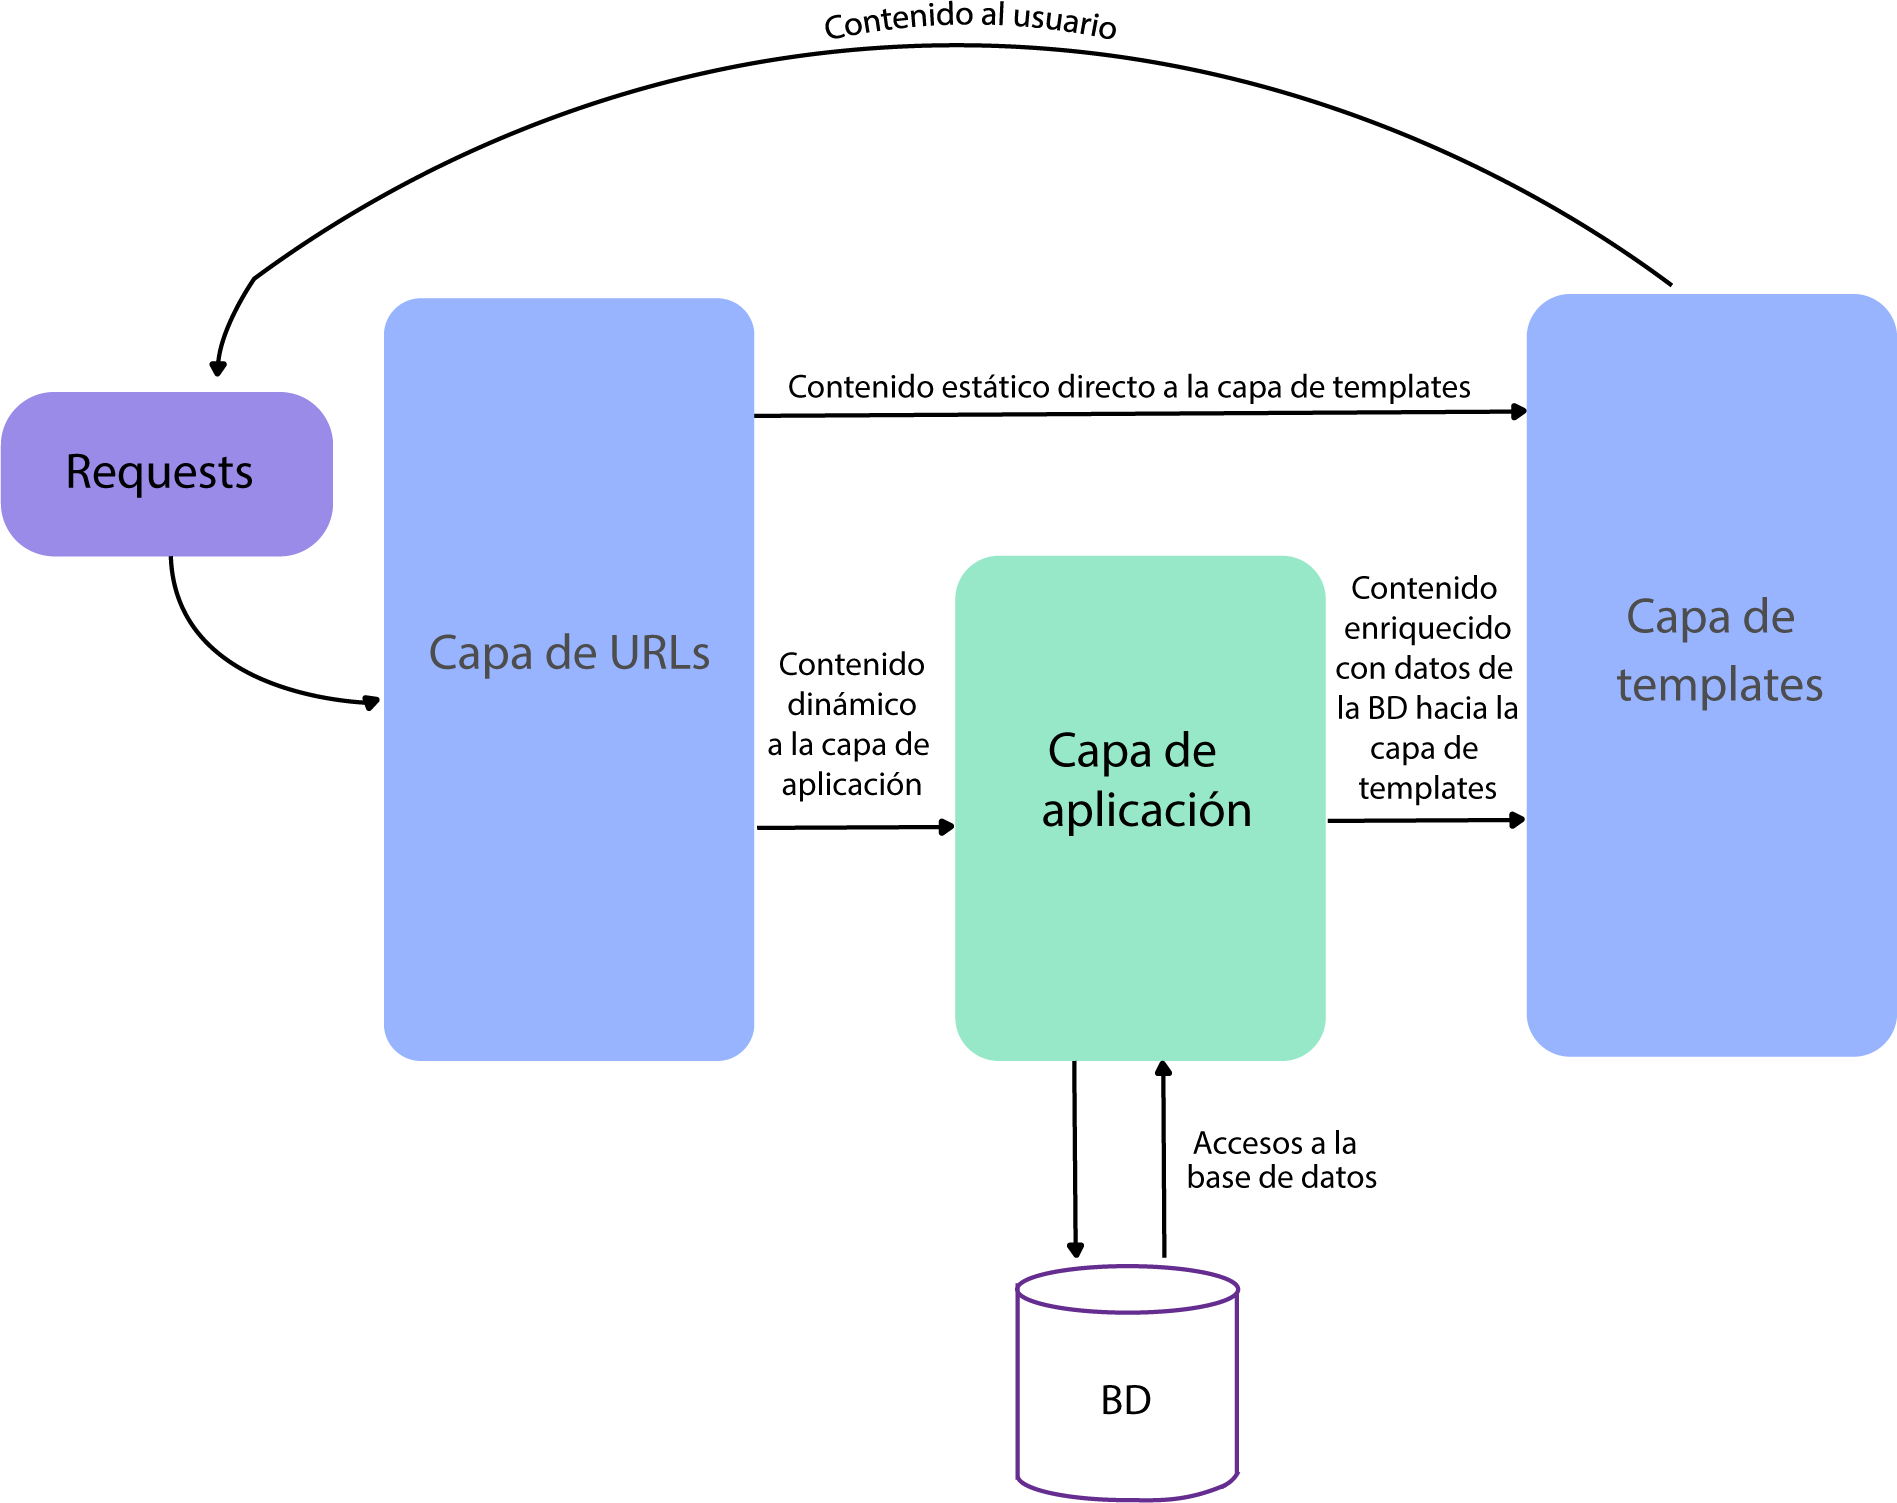
\includegraphics[scale=0.9]{images/django.png}
  \captionof{figure}{Flujo de trabajo de Django}
  \label{fig:django}
\end{figure}

Como se puede ver en la figura, hay dos flujos de información. Uno para enviar información estática, y el otro para enviar información dinámica.

\section[Flask]{Flask}

Flask es un framework chico para casi cualquier estándar. Suficientemente chico para que sea llamado "micro-framework"\cite{Fsck}. Pero ser chico no significa que hace menos que otros frameworks, sino que fue diseñado para ser extensible desde los cimientos. Provee un núcleo sólido con los servicios básicos, mientras el resto puede ser provisto por extensiones. El hecho de que permita elegir y poner la extensión que se desee, hace que se termine usando un framework que no tiene funcionalidades de más y sirve para exactamente lo que se necesite.
Flask tiene tres dependencias principales: rutas, debugging y WSGI (Web Server Gateway Interface, provisto por Werkzeug); los templates son provistos por Jinja2, y la interacción por línea de comandos viene de Click. Estas dependencias fueron escritas por Armin Ronacher, el autor de Flask.
Flask no dispone de acceso nativo a bases de datos, validar formularios web, autenticación, u otras tareas de alto nivel. Sólo se pueden usar a través de extensiones. Como desarrollador, se puede decidir integrar la que se desee o escribir una propia. Esto va en contraste con grandes frameworks, ya que es complejo o imposible cambiar estas funcionalidades.

\section[Python en Data Science]{Python en Data Science}

La comunidad de la ciencia de datos está cambiando de R a Python, ya que provee a los científicos una gran cantidad de funcionalidades y les permite crear sus propias funcionalidades para realizar cálculos muy complejos. Además, les permite generar varios tipos de reportes de análisis, histogramas, grafos, y mucho más.
Existen muchos módulos de Data Science, entre ellos numpy, Pandas, etc.

\subsection[Numpy]{Numpy}

NumPy, abreviatura de Numerical Python, viene siendo hace mucho tiempo una parte fundamental para la computación numérica. Provee estructuras de datos, algoritmos y liberías necesarias para la mayoría de las aplicaciónes científicas que involucran datos numéricos en Python. NumPy contiene entre otras cosas:
\begin{outline}
    \1 ndarray: Un array multidimensional rápido y eficiente.
    \1 Funciones para realizar cálculos basados en elementos con matrices u operaciones matemáticas entre matrices
    \1 Herramientas para leer y escribir datasets al disco.
    \1 Operaciones de álgebra lineal y generación de números aleatorios.
    \1 Una API en C muy madura que permite a las extensiones de Python acceder a las estructuras de datos de NumPy
\end{outline}
Mas allá de las capacidades de procesamiento de matrices que NumPy le agrega a Python, una de sus principales usos para análisis de datos es como contenedor para que los datos sean pasados entre algoritmos y librerías. Para datos numéricos, los arrays de NumPy son más eficientes para guardar y manipular los datos que cualquier otrá librería de Python.


\subsection[Pandas]{Pandas}

Pandas provee estructuras de datos de alto nivel y funciones diseñadas para trabajar con datos estructurados o tabulados de forma rápida, fácil y expresiva. Desde su salida en 2010 fue ayudando a Python a crear un entorno de análisis de datos poderoso y productivo. Los objetos principales de pandas son: 
\begin{outline}
    \1 DataFrame: una estructura de datos tabular, orientada a columnas, con etiquetas por columna y fila.
    \1 Series: un array etiquetado de una dimensión.
\end{outline}

Pandas mezcla la alta performance de las ideas computacionales sobre arrays de Numpy, con las capacidades flexibles de la manipulación de datos de las hojas de cálculos y las bases de datos relacionales (como SQL). Además, provee funcionalidades de indexación sofisticadas para que resulte fácil la remodelación, corte, agregación y selección de subconjunto de datos.

Pandas surgió en 2008 para cumplir con ciertos requerimientos que ninguna otra herramienta podía satisfacer:

\begin{outline}
    \1 Estructuras de datos con ejes etiquetados, y que soporte alineación de datos automática o explícita. Esto previene errores comunes resultantes de trabajar con datos provenientes de distintas fuentes.
    \1 Series de tiempo integradas.
    \1 Estructura de datos que pueda manejar series de tiempo y otros datos a la vez.
    \1 Operaciones aritméticas y reducciones que preserven los metadatos.
    \1 Manejo de datos faltantes de forma flexible.
    \1 Unión y otras operaciones relacionales encontradas en bases de datos.
\end{outline}

\section[React]{React}

React es una librería de Javascript que tiene como propósito simplificar el desarrollo de interfaces visuales.
Fue desarrollado por Facebook y lanzado al mundo en 2013.
Su objetivo principal es facilitar el razonamiento sobre las interfaces y su estado en cualquier momento, dividiendo la UI en una colección de componentes.

\subsection[Componente]{Componente}

Los componentes permiten separar la interfaz de usuario en piezas independientes, reutilizables y pensar en cada pieza de forma aislada.
Conceptualmente, los componentes son como las funciones de JavaScript. Aceptan entradas arbitrarias (llamadas “props”) y devuelven a React elementos que describen lo que debe aparecer en la pantalla.
Los componentes pueden referirse a otros componentes en su salida. Esto nos permite utilizar la misma abstracción de componente para cualquier nivel de detalle. Un botón, un cuadro de diálogo, un formulario, una pantalla: en aplicaciones de React, todos son expresados comúnmente como componentes.


\subsection[DOM Virtual]{Dom Virtual}

DOM (Document Object Model) es un arbol que representa una página, empezando con la etiqueta <html>, bajando por cada hijo llamado nodo.
Se guarda en la memoria del navegador y se vincula directamente con lo que se ve en una página. El DOM tiene una API, con la cual se puede acceder a él, acceder a cada nodo, filtrarlos, modificarlos.
React mantiene una copia de la representación del DOM al que llama DOM virtual.

Cada vez que el DOM cambia, el navegador tiene que realizar dos operaciones intensivas: repintar (cambios visuales o de contenido en un elemento que no afectan el diseño y el posicionamiento en relación con otros elementos) y reflujo (recalcular el diseño de una parte de la página, o el diseño completo de la página).
React usa DOM Virtual para ayudar al navegador a usar menos recursos cuando se necesita que haya cambios en la página.

React sólo cambia el DOM cuando el estado de un componente cambia explícitamente.
Cuando hay un cambio, React actualiza el DOM Virtual relativo al componente que necesita cambiar.
La clave está en que sólo actualiza el DOM una vez, asi el "repintado" y "reflujo" que tiene que realizar el navegador se hace sólo una vez.


\section[Microservicios]{Microservicios}

Los microservicios son servicios pequeños y autónomos que trabajan en conjunto. 
A medida que el código va creciendo cuando se agregan funcionalidades, se hace cada vez complejo saber dónde se tienen que hacer los cambios.
Las funcionalidades nuevas empiezan a quedar esparcidas por todo el código, haciendo que sea cada vez más dificil encontrar errores.

Los microservicios afrontan un acercamiento hacia la independencia de servicios. Enfocandose en la obviedad donde el código solo sirve para alguna funcionalidad. Y al mantener este servicio enfocado dentro de sus límites, se evita que crezca demasiado.

\subsection[Heterogeneidad Tecnológica]{Heterogeneidad Tecnológica}

Con un sistema compuesto de multiples servicios colaborando entre sí, podemos elegir usar diferentes tecnologías dentro de cada uno de éstos. Esto permite elegir la herramienta correcta para cada trabajo, en lugar de tener que elegir una opción que sirva un poco para todo, y puede terminar siendo perjudicial para el sistema.

Si una parte del sistema necesita mejorar su performance, podemos decidir cambiar de tecnología a una que resulte mejor para esa tarea en particular.

\begin{figure}[h!]
  \centering
    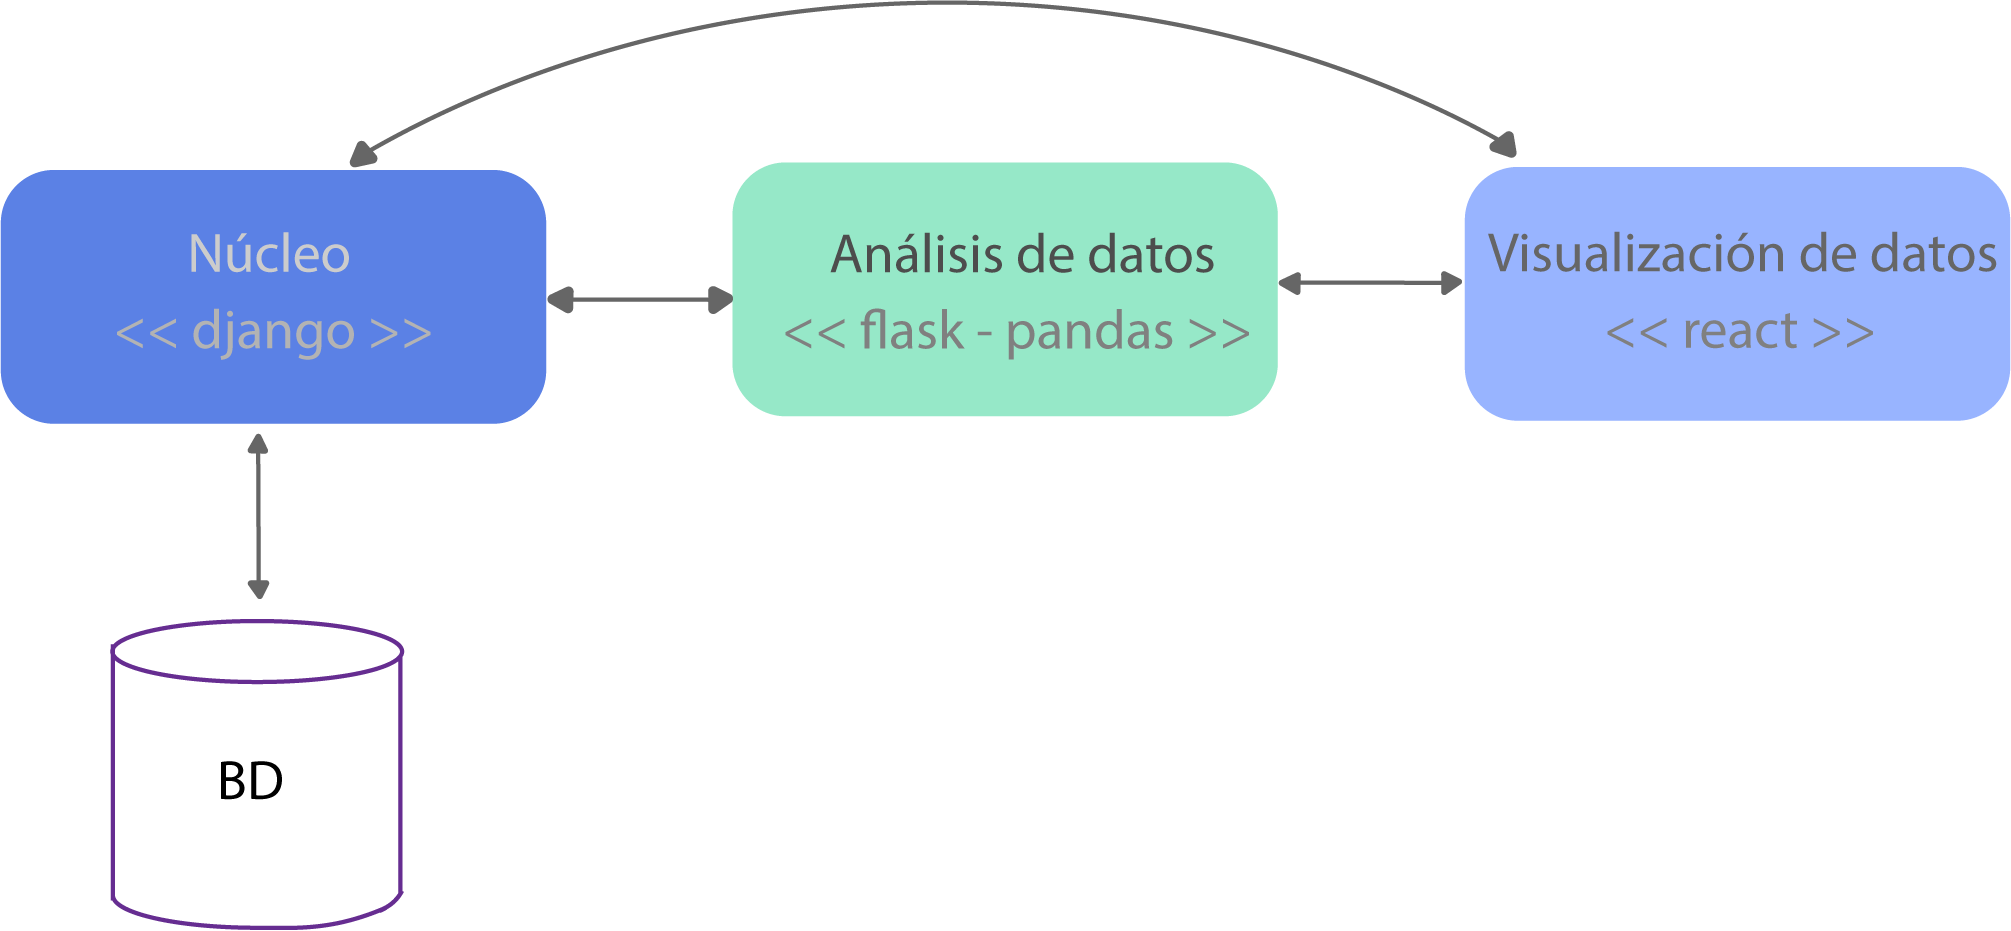
\includegraphics{images/heterogeneidad-tecnologica.png}
  \captionof{figure}{Microservicios: Homogeneidad Tecnológica}
  \label{fig:microht}
\end{figure}

\break

El gráfico muestra tres servicios distintos, un núcleo que usa Django, un servicio de análisis de datos, con Flask y Pandas, y un servicio de visualización de datos con React.

\subsection[Independencia]{Independencia}

En un sistema monolítico, cuando hay una falla todo el sistema se corrompe. Aunque se pueda mitigar usando varias instancias del mismo sistema, esto no es conveniente ya que a medida que el sistema va creciendo, tener varias instancias de un sistema grande necesitaría una mayor capacidad de procesamiento.
Desde la perspectiva de microservicios, cuando uno de los servicios tenga una falla y esa falla no genere un problema en cascada, se puede aislar el problema y así el resto de los servicios puede seguir funcionando. 

\subsection[Escalamiento]{Escalamiento}

En un sistema monolítico, todo se escala junto. Si sólo se necesitara que un servicio determinado tenga mas recursos, estaría dándole más recursos a todo el sistema.
En cambio, con microservicios, si en un determinado momento se necesita, por ejemplo, que el servicio de análisis de datos procese mas peticiones se podría escalar sólo ese servicio teniendo dos instancias (o más) de esa parte del sistema, dejando los otros módulos corriendo con hardware menos poderoso, acorde a sus necesidades.

\begin{figure}[h!]
  \centering
    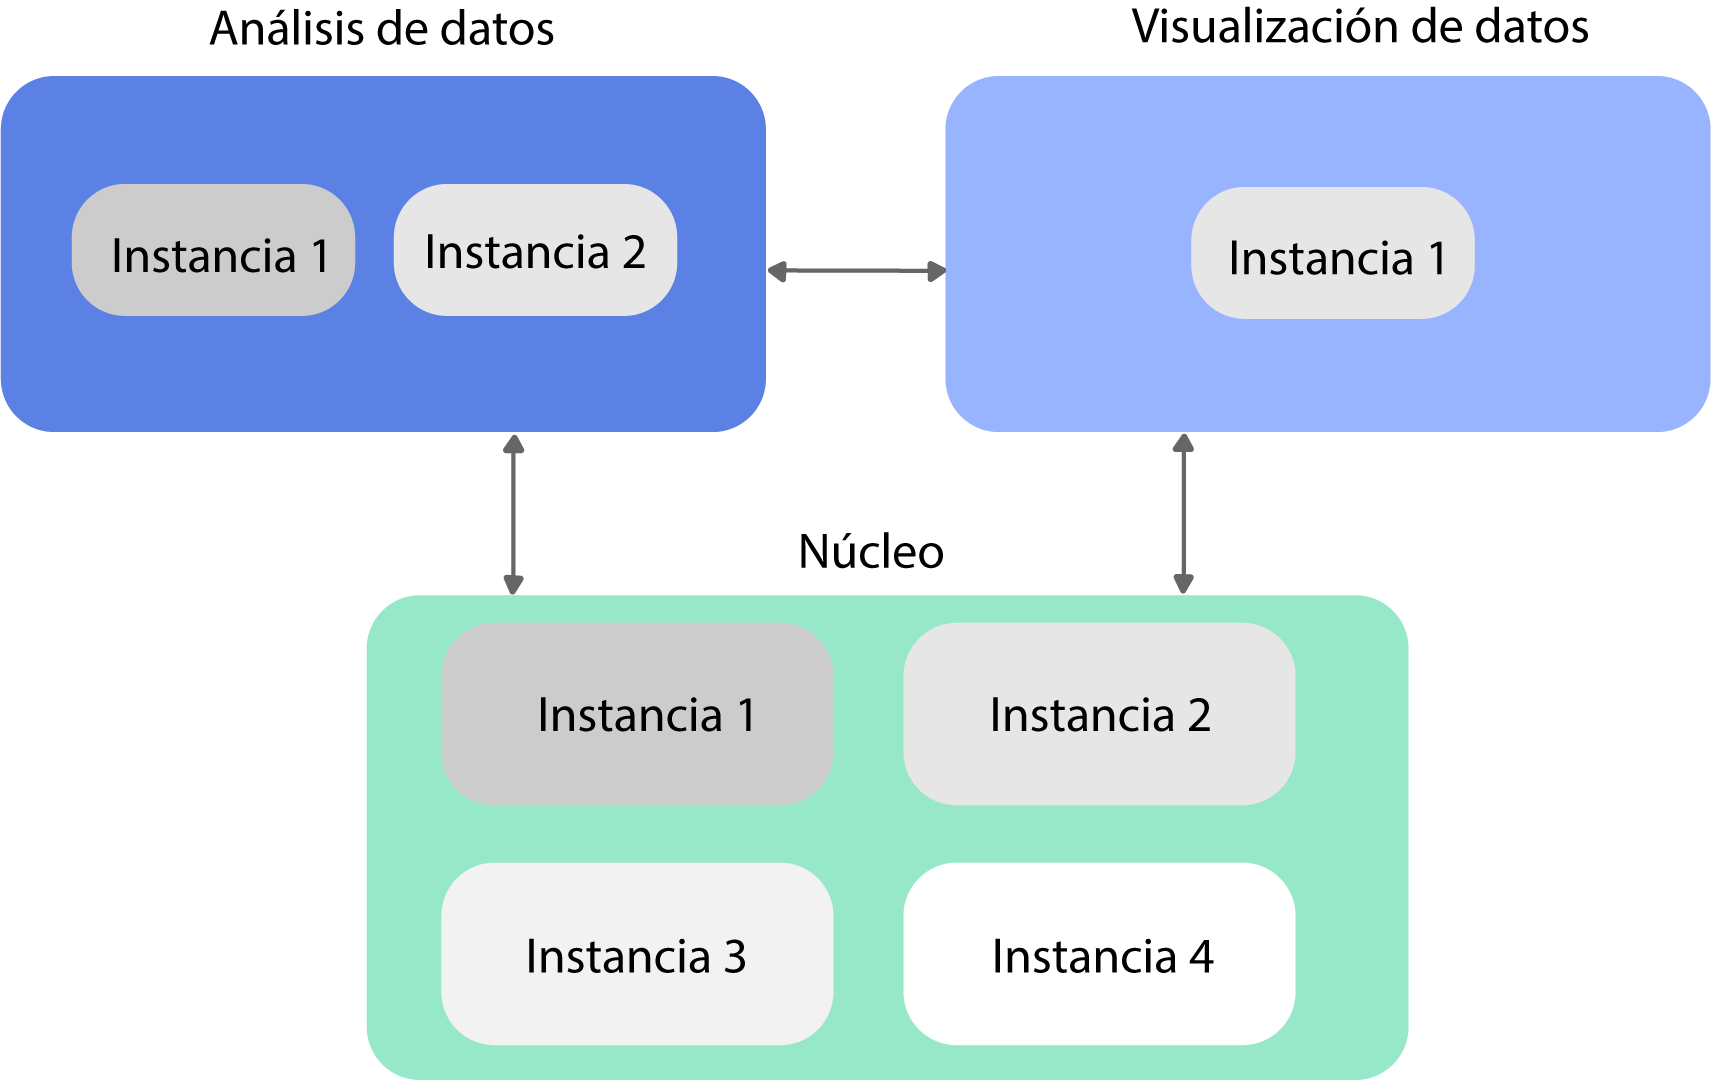
\includegraphics[scale=0.7]{images/escalamiento.png}
  \captionof{figure}{Microservicios: escalamiento}
  \label{fig:microescala}
\end{figure}

\subsection[Facilitar deploy]{Facilitar deploy}

Hacer un pequeño cambio en un sistema monolítico requeriría deployar toda la aplicación para hacer efectivo el cambio. Esto genera un gran impacto y un alto riesgo. 
Desde la perspectiva de los microservicios, el cambio que se hace sobre un servicio permite deployar sólo ese módulo, sin que los otros sepan que hubo una modificación. Además, el código es deployado mas rápido. 
De haber un problema en la actualización, se puede aislar a un sólo servicio, permitiendo retroceder a una versión anterior.

\subsection[Reemplazabilidad]{Reemplazabilidad}

El costo de reemplazar un servicio por una mejor implementación es más fácil de manejar cuando hay independencia. 
Si en un futuro se quisiera, por ejemplo, cambiar el módulo de encuestas, sólo haría falta reemplazar ese pequeño sistema sin tener que modificar el resto. Ni siquiera deberian enterarse del cambio.

>> Gráfico conceptual del nucleo y otras apps

\section[REST]{Rest}

REpresentational State Transfer (Transferencia de estado representacional, su traducción) es un estilo arquitectural inspirado en la Web. 
Una parte importante es el concepto de **recursos**. 
El servidor crea diferentes representaciones del recurso en un request. La forma en que es enviado esta desacoplado a cómo está guardado internamente. Cuando un cliente pide por un recurso, se le da una representación con la estructura de JSON.
A lo largo de los años, se desarrollaron muchos servicios basados en la arquitectura REST, que usa las funcionalidades provistas por la capa de aplicación del protocolo HTTP \cite{RestSoap} \cite{IETF}. Esto resultó en un incremento en el interés comparado al tradicional SOAP (Simple Object Access Protocol). Además, grandes compañías como Twitter o Amazon usan interfaces del tipo REST en sus servicios, lo cual se puede ver en la documentación de sus APIs (Application Programming Interface).
Mas allá de la tendencia, no hay estándares o guias de cómo desarrollar un servicio web RESTful. En lugar de esto, existen buenas prácticas.

\subsection[No versionado]{No versionado}

Versionar una API Web es una de las consideraciones más importantes a la hora de diseñar un servicio web, ya que la API representa el punto de acceso al servicio y oculta su implementación. Es por esto que una interfaz web nunca deberia ser desplegada sin un identificador de version \cite{WAPID}. Para versionar, existen diferentes acercamientos como incluirlo en la URI (Uniform Resource Identifier) del servicio web o usando el header HTTP para seleccionar la versión apropiada \cite{WAPID}. Pero el servicio web basado en REST no necesita ser versionado debido a hipermedia. Es por esto que los servicios web RESTful pueden ser comparados con los sitios web tradicionales, que pueden ser accedidos por todos los navegadores cuando se cambia el contenido del sitio. Asi que no sería necesario agregar información del lado del cliente.
Mas allá de esto, el uso de versionado genera un impacto negativo en los servicios web ya desplegados, ya que aumenta el esfuerzo por mantenerlos.


\subsection[Descripción de los recursos]{Descripción de los recursos}

La descripción de los recursos se relaciona con la usabilidad de los servicios web, ya que éstos son una representación del modelo. Para una correcta descripción, existen algunas buenas prácticas:
\begin{outline}
    \1 Deberían usarse sustantivos para los recursos \cite{WAPID}.
    \1 El nombre del recurso debería ser un nombre específico del dominio, para que la semántica pueda ser interpretada por cualquier usuario sin conocimientos adicionales \cite{WAPID}
    \1 Debería evitarse la mezcla del uso del plural y singular para garantizar coherencia \cite{WAPID}.
    \1 Debería usarse la convención de nombres de JavaScript, ya que el tipo JavaScript Object Notation (JSON) es el tipo de dato más usado para la comunicación entre el cliente y el servidor \cite{WAPID}.
\end{outline}
\subsection[Identificación de recursos]{Identificación de recursos}

Deberían usarse URIs para la identificación única de recursos \cite{ASDNB}. Para esto existen algunas buenas prácticas:
\begin{outline}
    \1 Una URI debería ser autoexplicativa, de forma tal que no debería necesitar información adicional para su uso \cite{WAPID}.
    \1 No deberían existir verbos en la URI, ya que esto implica una orientación a métodos como SOAP \cite{WAPID}.
    \1 Un recurso debería ser represantado por dos URIs. La primera para representar el conjunto de estados de un recurso específico, y la segunda para representar un estado en particular de ese conjunto de estados \cite{WAPID}.
    \1 El identificador de un estado específico debería ser dificil de predecir y no referenciar objetos directamente, según OWASP (Open Web Application Security Project), si no existiera una capa de seguridad.
\end{outline}

\subsection[Manejo de errores]{Manejo de errores}

Los mensajes de error tienen que ser claros y entendibles, para que su causa pueda ser fácilmente identificada. Con esto en mente, se pueden reconocer algunas buenas prácticas:
\begin{outline}
    \1 La cantidad de códigos de estados de HTTP debería estar limitado para reducir el esfuerzo de buscar en la especificación \cite{WAPID}.
    \1 El uso de los códigos de estado de HTTP tienen que corresponderse con la especificación oficial de HTTP \cite{HTTP}.
    \1 Debería darse un mensaje de error detallado como una pista del error causado del lado del cliente \cite{WAPID}. Por este motivo, el mensaje de error debería tener los siguientes ingredientes:
        \2 Un mensaje para los desarrolladores, que describe la causa del error y algunas pistas sobre cómo resolver el problema.
        \2 Un mensaje que puede ser mostrado al usuario
        \2 Un código de error específico de la aplicación
        \2 Un link para más información sobre el problema.
\end{outline}
\subsection[Uso de parámetros]{Uso de parámetros}

Cada URI de un recurso puede ser extendida con parámetros para proveer información opcional al servicio. A continuación se detallan cuatro casos de uso:
\begin{outline}
    \1 Filtrado: para filtrar información de un recurso, puede usarse sus atributos o algun lenguaje de queries. La elección de una de estas variantes, depende de la necesidad del poder de expresión que se tenga para filtrar. 
    \1 Ordenamiento: para ordenar la información, se recomienda \cite{BPRA} una lista de atributos separados por coma con el parámetro "sort" en la URI, seguido por un signo de más (+) como prefijo para un orden ascendente, o un signo menos (-) para un orden descendente.
    \1 Selección: la selección de información en forma de atributos reduce el tamaño de transmisión sobre la red, respondiendo sólo con la información pedida. Para este propósito, se recomienda una lista de atributos separadas por coma.
    \1 Paginación: La paginación permite partir la información en varias páginas virtuales, mientras se referencian la página anterior, la próxima, la primera y la última. 
\end{outline}
\subsection[Interacción con los recursos]{Interacción con los recursos}

Usando REST como el estilo de arquitectura subyacente de un sistema, el cliente interactúa con las representaciones de un recurso en lugar de usarlo directamente. La interacción entre el cliente y el servidor esta construido en la capa de aplicación del protocolo HTTP, que ya provee cierta funcionalidad para la comunicación. Para la interacción con un recurso, podriamos identificar tres buenas practicas diferentes:
\begin{outline}
    \1 El uso de los métodos HTTP deberían ser de acuerdo a las semánticas definidas por la especificación oficial de HTTP \cite{WAPID}. Así, el método GET de HTTP sólo debería ser usado para las operaciones sin efectos secundarios. Para una mejor visión general, la tabla a continuación muestra los métodos HTTP mas usados y sus características. Estas características pueden ser usadas para asociar los métodos HTTP con el correcto uso de la creación, lectura, edición y borrado de recursos (CRUD) \cite{RVINOSKI}.
    \1 El soporte de la operación OPTIONS es recomendada si una gran cantidad de datos tienen que ser transmitidos, ya que permite al cliente pedir los métodos soportados de la representación actual antes de transmitir la información por un medio compartido. 
    \1 El soporte del GET condicional debería ser considerado durante el desarrollo de un servicio basado en HTTP, ya que previene al servidor de tranmitir datos ya enviados anteriormente. Solo si hay modificaciones de la información solicitada desde la última solicitud, el servidor responde con la última representación  \cite{RVINOSKI}.
\end{outline}

\begin{table}[]
    \centering
    \makegapedcells
    \begin{tabular}{|c|c|c|}
    \hline
    Método & Seguro & Idempotente \\ \hline
    POST & No & No \\ \hline
    GET & Si & Si \\ \hline
    PUT & No & Si \\ \hline
    DELETE & No & Si \\ \hline
    
    \end{tabular}
    \caption{Características de los métodos HTTP más comúnes}
    \label{tab:tabla_planes}
\end{table}

\subsection[REST y HTTP]{REST y HTTP}
HTTP define algunas funcionalidades que son muy útiles para REST. Por ejemplo los verbos (GET, POST, PUT, etc) ya tienen un buen entendimiento sobre cómo deberian funcionar con recursos. El estilo de arquitectura REST nos dice que los métodos deberian comportarse de la misma forma en todos los recursos, y la especificación HTTP define muchos de estos métodos. 
GET sirve para pedir recursos y POST para crear (aunque para el sistema seguimiento académico de no todos los recursos van a poder ser creados).
HTTP también trae un gran ecosistema de herramientas y tecnologías que facilitan la tarea. 


\section[JSON Web Tokens (JWT)]{JSON Web Tokens (JWT)}
\subsection[¿Qué es?]{¿Qué es?}

JSON Web Token es un estándar abierto (RFC 7519) que define una forma compacta de transmitir informacion entre partes de forma segura como un objeto JSON. Esta información puede ser verificada y confiada porque está firmada digitalmente. JWT puede ser firmado usando una clave secreta (con el algoritmo HMAC) o un par de claves pública/privada usando RSA o ECDSA.


\subsection[¿Cuándo usarlo?]{¿Cuándo usarlo?}

Estos son algunos escenarios donde JWT es útil:
\begin{outline}
    \1 Autorización: Este es el escenario mas común. Una vez que el usuario esta logueado, cada request que se haga debe incluir el JWT, permitiendo al usuario acceder a rutas, servicios y recursos que se le son permitidos con ese token. Single Sign On es una funcionalidad que usa mucho JWT, por su habilidad de poder ser usado a través de diferentes dominios.
    \1 Intercambio de información: JSON Web Tokens son una forma segura de transmitir informacion entre partes. Como están firmados, se puede estar seguro que el emisor es quien dice que es. Además, como la firma es calculada usando el "header" y el "payload", se puede verificar que el contenido no fue modificado.
\end{outline}
\subsection[Estructura]{Estructura}


En su forma compacta, los JSON Web Tokens consisten de tres partes separadas por puntos (.), que son:
\begin{outline}
    \2 Header
    \2 Payload
    \2 Firma
\end{outline}

\subsection[Header]{Header}

El header consiste de dos partes: el tipo de token, que es JWT, y el algoritmo que se usa para firmar, como HMAC SHA256.

\begin{lstlisting}[language=json,firstnumber=1]
{
"typ": "JWT",
"alg": "HS256"
}
\end{lstlisting}
Luego, este JSON es encodeado con Base64Url para formar la primer parte del JWT.

\subsection[Payload]{Payload}

La segunda parte del token es el payload, que contiene los pedidos. Un pedido es una declaración sobre una entidad (por lo general, un usuario) e información adicional. Hay tres tipos de pedidos: registrados, públicados y privados.

\begin{outline}
    \1 Registrados: Estos son un conjunto de pedidos predefinidos, que no son obligatorios pero recomendados para proveer información útil. Algunos de estos son: iss (issuer), exp (fecha de expiración del token), sub (asunto), aud (audiencia), y otros.
    \1 Públicos: Esta parte es definida por quien use el JWT. Pero para evitar colisiones, deberian estar definidos en el registro IANA o estar definidos como una URI que contiene un nombre resistente a colision.
    \1 Privados: Estos son campos personalizados, con la finalidad de compartir información entre partes.
\end{outline}

Un ejemplo de payload puede ser: 

\begin{lstlisting}[language=json,firstnumber=1]
{
  "token_type": "refresh",
  "exp": 1582059853,
  "jti": "e9b85778f3f44decba69a611e4e1c700",
  "user_id": 1,
  "carreras": [
    "W"
  ],
  "username": "admin"
}
\end{lstlisting}

El payload luego es encodeado con Base64Url para formar la segunda parte del JWT.

\subsection[Firma]{Firma}

Para crear la parte de la firma, se usa el header encodeado, el payload encodeado, una clave secreta, y el algoritmo especificado en el hader, y firmar eso.
Por ejemplo, usando el algoritmo HMAC SHA256, la firma se crea de la siguiente forma: 

\begin{lstlisting}[language=Python]
HMACSHA256(
    base64UrlEncode(header) + "." +
    base64UrlEncode(payload),
    clave-secreta
)
\end{lstlisting}
La firma es usada para verificar que el mensaje no fue cambiado en el camino, y también para verificar que el emisor es quien dice ser.

\subsection[Poniendo todo junto]{Poniendo todo junto}

El resultado van a ser tres strings en Base64Url, separados por puntos que pueden ser fácilmente pasados por HTTP, siendo muy compactos comparado con estándares XML como SAML.

The output is three Base64-URL strings separated by dots that can be easily passed in HTML and HTTP environments, while being more compact when compared to XML-based standards such as SAML.

Lo siguiente muestra un JWT formado con las tres partes provistas:


eyJhbGciOiJIUzI1NiIsInR5cCI6IkpXVCJ9.\break eyJ0b2tlbl90eXBlIjoicmVmcmVzaCIsImV4cCI6MTU4MjA1OTg1MywianRpIj\break oiZTliODU3NzhmM2Y0NGRlY2JhNjlhNjExZTRlMWM3MDAiLCJ1c2VyX2lkIj\break oxLCJjYXJyZXJhcyI6WyJXIl0sInVzZXJuYW1lIjoiYWRtaW4ifQ.\break KryBoqAQpHNliUUw3-xLJE2u4M6_tBByJQtf7IFYQis



\subsection[¿Cómo funciona?]{¿Cómo funciona?}

En autenticación, cuando el usuario se loguea usando sus credenciales, se le provee un JSON Web Token. Como es una credencial, se debe tener cuidado con los problemas de seguridad que se puedan tener. En general, no se deben mantener tokens mas tiempo del requerido. Tampoco se tiene que guardar datos sensibles de sesiones en el almacenamiento del navegador.
Cuando un usuario quiere ingresar a una ruta o un recurso protegido, tiene que mandar el JWT en el header de autorización, usando el esquema "Bearer". El contenido del header tiene que verse como lo siguiente:
\begin{lstlisting}[language=Python]
Authorization: Bearer <token>
\end{lstlisting}

Este puede ser un mecanismo de autorización sin estado. Las rutas protegidas del servidor chequean que el JWT sea válido. Si lo es, el usuario puede ingresar a esas rutas protegidas. Si el JWT tiene los datos necesarios, se reducen las queries a la base de datos, aunque no siempre sea el caso.
Si el token es enviado en el header de autorización, Cross-Origin Resource Sharing (CORS) no va a ser un problema ya que no usa cookies.

>> Gráfico de pedido de token



\subsection[Problemas que resuelve]{Problemas que resuelve}

A pesar de que el principal propósito de JWTs es transferir demandas entre dos partes, el aspecto más importante es el de estandarizar una estructura de datos de forma simple y encriptada. 
Los principales problemas que resuelve son:
\begin{outline}
\2 Autenticación
\2 Autorización
\2 Identidad Federada
\2 Sesiones del lado del cliente
\end{outline}

\subsection[Client-side/Stateless Sessions]{Client-side/Stateless Sessions]}

Las llamadas sesiones sin estado (stateless sessions) son en realidad datos del lado del cliente (client-side). El aspecto fundamental de esta aplicación reside en el uso de firmas y posiblemente encriptación para proteger el contenido de la sesion. Como los datos del lado del cliente pueden ser manipulados con facilidad. Por esta razón, se tiene que tener mucho cuidado desde el backend.

JWTs, en virtud de JWS y JWE, puede proveer distintos tipos de firmas y encriptación. Las firmas son útiles para validar los datos contra posibles manipulaciones. La encriptación es útil para proteger los datos de ser leídos por terceros.

\subsection[¿Es útil tener una sesión del lado del cliente?]{¿Es útil tener una sesión del lado del cliente?}

Existen pros y contras a cualquier decisión, y las sesiones client-side no son la excepción. Algunas aplicaciones pueden requerir sesiones muy grandes. Enviando este estado ida y vuelta hacia el backend por cada request (o grupo de requests) puede vencer rápidamente los beneficios que trae JWT. Es necesario un buen balance entre los datos del lado del cliente y las búsquedas a la base de datos del backend.

\subsection[Tokens de acceso y refresh]{Tokens de acceso y refresh}

Los tokens de acceso (access) y refresh son dos tipos de tokens que ayudan en el contexto de autenticación y autorización.

Los tokens de acceso son tokens que dan a aquel que lo tenga, el acceso a recursos protegidos. Éstos tokens son de corta vida y tienen una fecha de expiración como dato. Tienen, además, otra información que puede ser de ayuda para identificar al cliente. Esta información adicional está definida en la implementación.

Por el contrario, los tokens de refresh le da permiso a los clientes que pidan un nuevo acceso. Por ejemplo, luego de que un token de acceso expiró, un cliente puede hacer un pedido de un nuevo acceso al servidor de autorización. Para que ésto pueda suceder, es requerido un token de refresh.
A diferencia de los tokens de acceso, el tiempo de vida del token de refresh suele ser largo.

La principal diferencia entre el token de acceso y el de refresh, está en la posibilidad de hacer los tokens de acceso fáciles de validar. Un token de acceso que tiene una firma, no hace falta que sea validado por un servidor de autorización.
Los tokens de refresh, por el contrario, necesita que se acceda al servidor de autorizaciones. Manteniendo la validación separada de las queries al servidor de autorización, es posible obtener una mejor latencia.
Para asegurar que la pérdida o robo de tokens no sea determinante, se debería poner un tiempo de vida corto.
Los tokens de refresh, al ser de vida prolongada, tienen que ser protegidos contra estas incidencias. 
Una opción es agregarlo a una lista negra y cuando alguien pida un access token, éste es expirado automáticamente.

\section[Docker]{Docker}

\subsection[Introducción]{Introducción}

Docker es una plataforma abierta para desarrollar, transportar, y ejecutar aplicaciones de forma rápida. Docker permite que las aplicaciones corran de forma separada de la infraestructura del host. Permite tambien enviar código, testear, desplegar rápido y acortar el ciclo entre escribir el código y correrlo. Docker loga esto combinando una plataforma de virtualización liviana con herramientas que permiten manejar y desplegar aplicaciones \cite{Dj}.

Docker usa funcionalidades del kernel de Linux como cgroups, que limita y aisla el uso de recursos, y namespaces, que permite a los contenedores independientes correr en una única instancia de Linux evitando la sobrecarga de iniciar máquinas virtuales.
Además, provee una forma para correr aplicaciones aisladas en un contenedor de forma segura, y que estos contenedores puedan correr de forma simultánea en un mismo host compartiendo el mismo kernel. Aunque cada contenedor puede usar una cantidad de recursos definidos por el host.

A diferencia de las máquinas virtuales, no se requiere un sistema operativo separado. Sino que depende de las funcionalidades del kernel y el uso aislado de recursos (CPU, memoria, I/O, red, etc).

\subsection[Imágenes y contenedores]{Imágenes y contenedores}

Un contenedor (container) es una versión de un sistema operativo Linux, solo con los componentes más básicos. Una imagen es un software que se carga dentro del contenedor al momento de ejecutar el comando run

\begin{lstlisting}[language=bash]
    docker run hello-world
\end{lstlisting}


El comando run recibe como parámetro requerido el nombre de la imágen que se desea cargar en un contenedor, en éste caso, hello-world.
Al correr dicho comando, Docker ejecuta las siguientes acciones:

- Comprobar que exista en el sistema una imágen con el nombre hello-world.
- En caso que no exista, se descarga desde el repositorio de imágenes configurado (por defecto es Docker Hub).
- Cargar la imágen en el contenedor y ejecutarla.

Por otro lado, una imágen de Docker puede ejecutar desde un simple comando hasta cargar un complejo sistema de base de datos.
Para construir una imágen, es necesario crear un archivo llamado Dockerfile.

\begin{lstlisting}
    FROM ubuntu:16.04
    RUN apt-get -y update
    CMD["echo Hola"]
\end{lstlisting}

El dockerfile anterior busca una imágen de Ubuntu con el tag 16.04. Luego ejecutará un comando para actualizar los paquetes del sistema operativo y finalmente mostrará el mensaje Hola.
El comando para construir una imágen de Docker es:

\begin{lstlisting}[language=bash]
    docker build -t nombre-imagen
\end{lstlisting}

Se ejecutará el comando build para construir la imágen. El argumento -t indica que se pondrá la etiqueta nombre-imagen a la imágen. El punto final indica el directorio de contexto de la imágen. En este caso, el contexto será el directorio donde se encuentra el Dockerfile.
Luego se carga la imágen en un contenedor con el comando:

\begin{lstlisting}[language=bash]
    docker run nombre-imagen
\end{lstlisting}


\subsection[Contenedor]{Contenedor}

Los contenedores y las máquinas virtuales tienen un aislamiento y asignación de recursos similar. Aunque funcionan diferente ya que los contenedores virtualizan el sistema operativo en lugar del hardware.

\begin{figure}[h!]
  \centering
    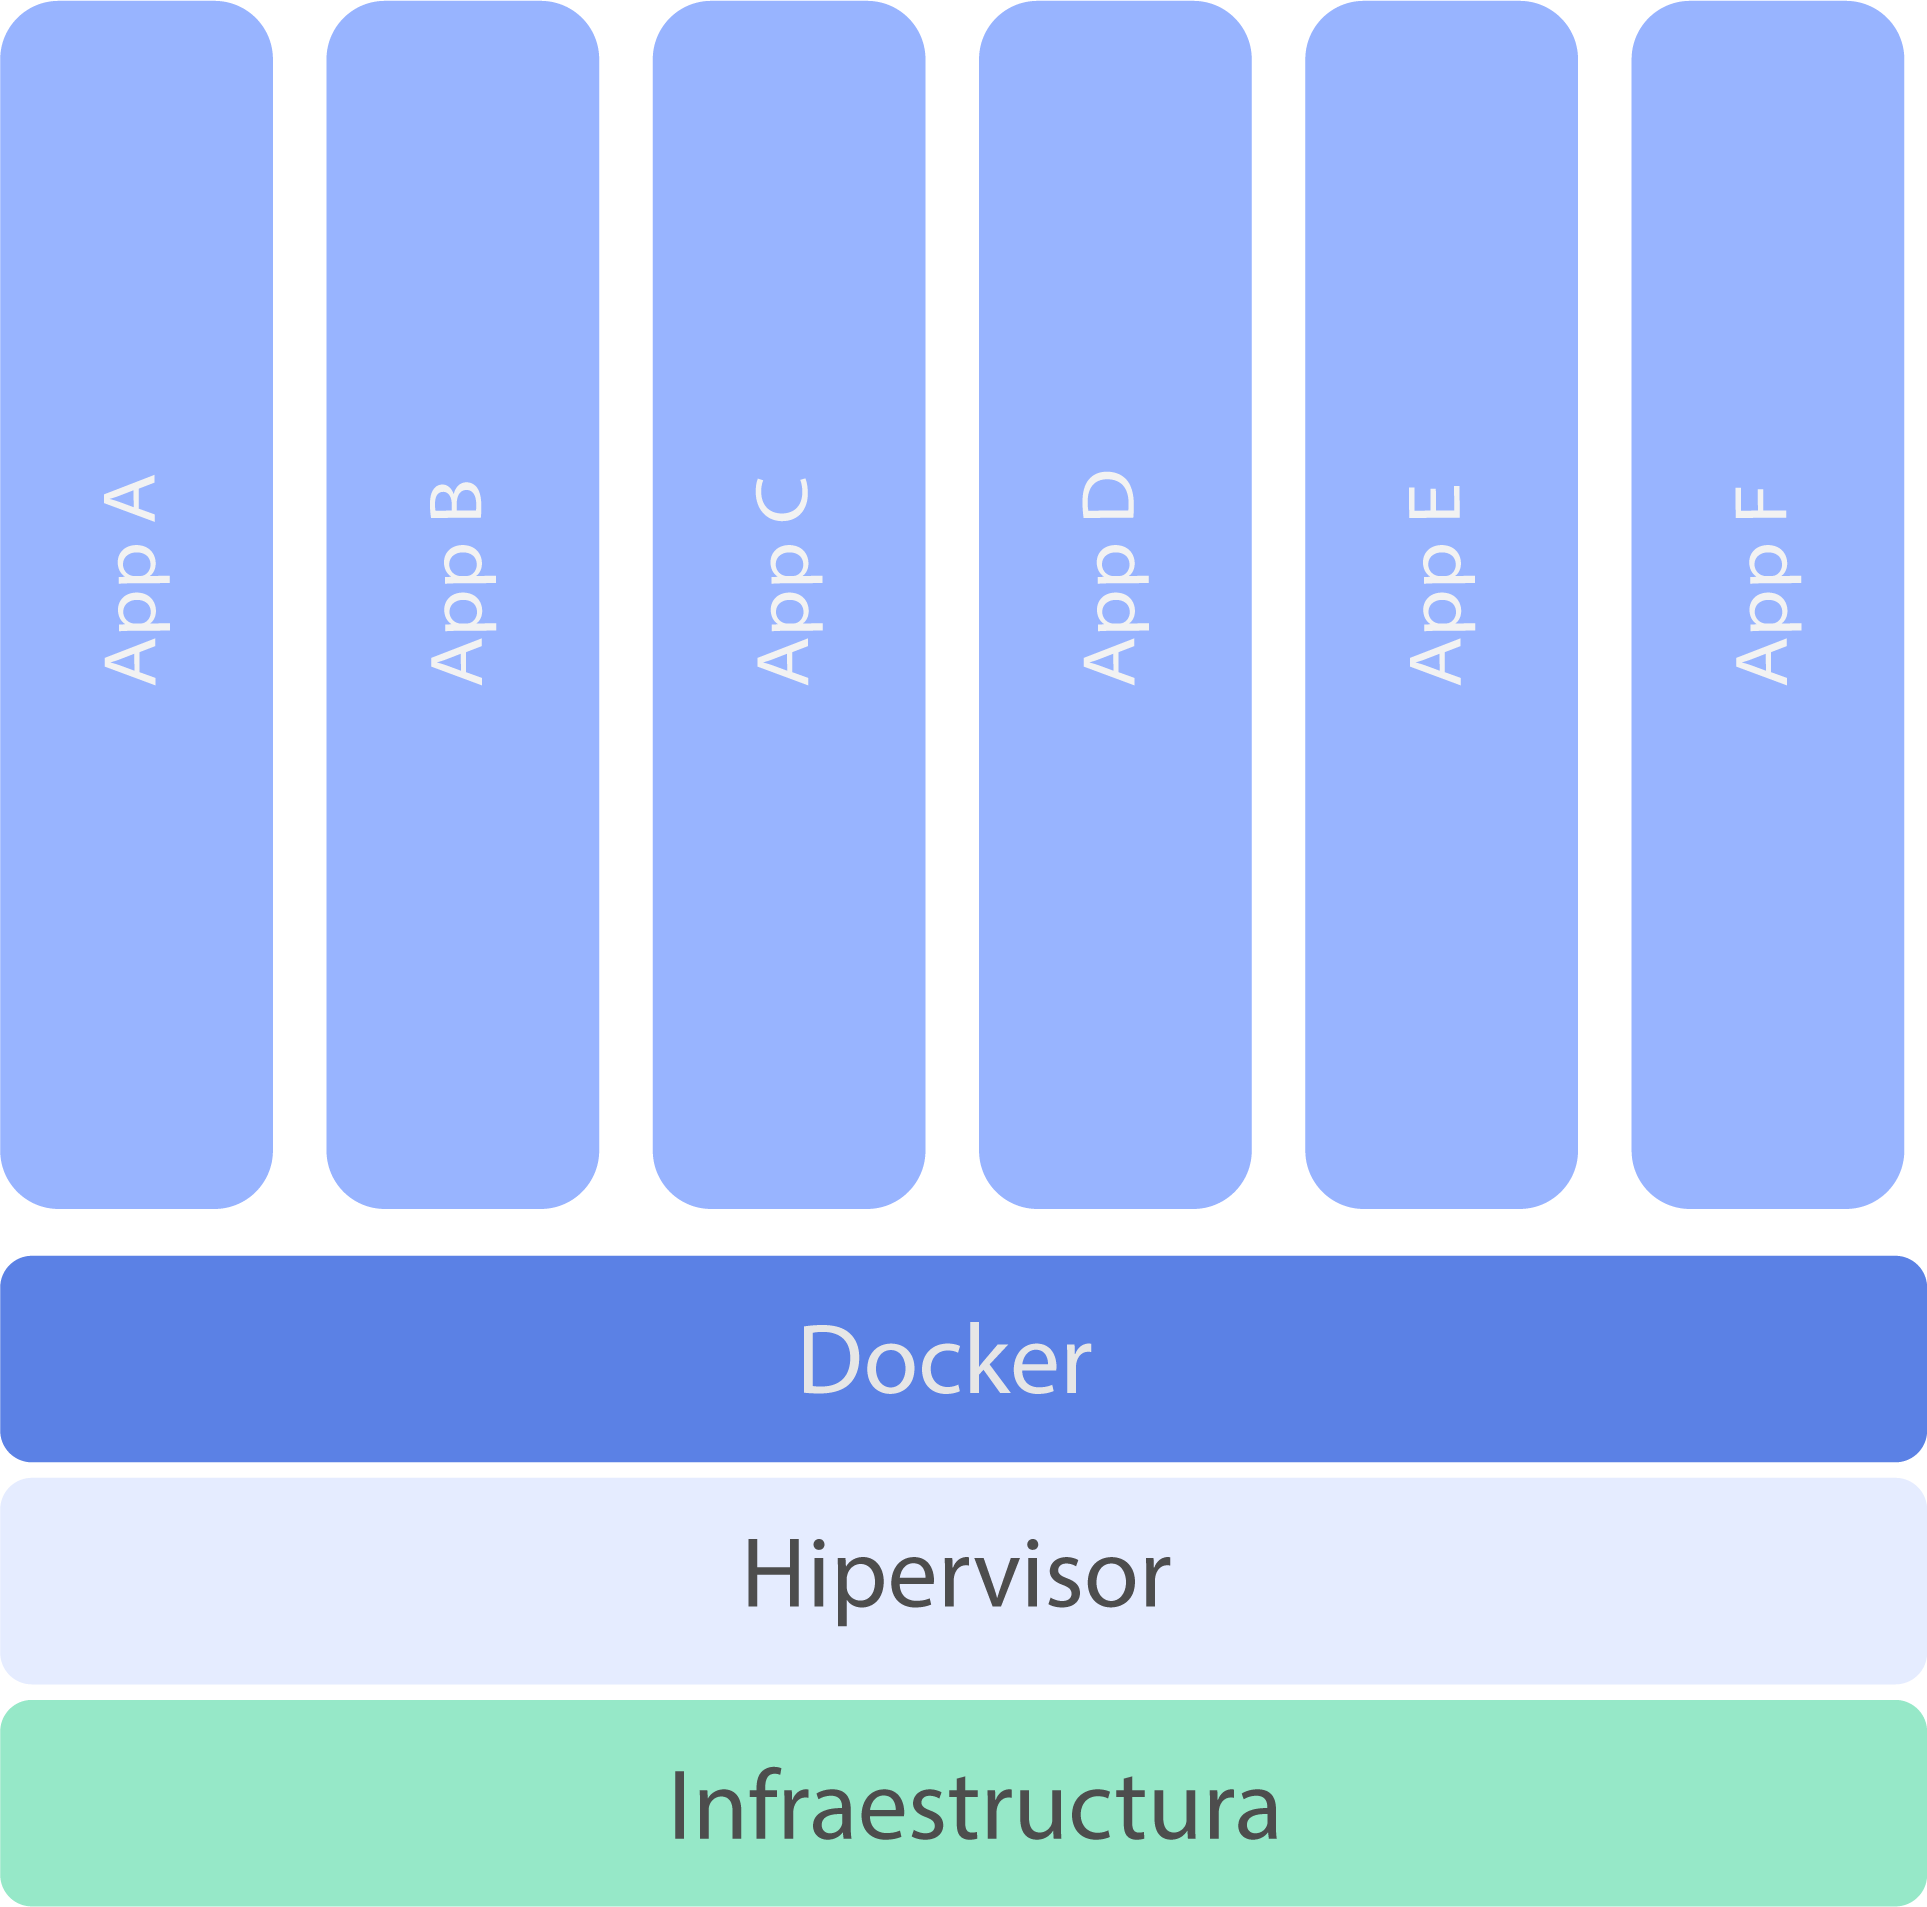
\includegraphics[scale=0.7]{images/containers.png}
  \captionof{figure}{Contenedor vs VM}
  \label{fig:contvm}
\end{figure}

\break

Los contenedores son una abstracción de la capa de aplicación que empaqueta el código y las dependencias juntos. Múltiples contenedores pueden correr en la misma máquina compartiendo el kernel del sistema operativo junto con otros contenedores, todos corriendo de forma aislada. Los contenedores ocupan menos espacio que las VMs.

\begin{figure}[h!]
  \centering
    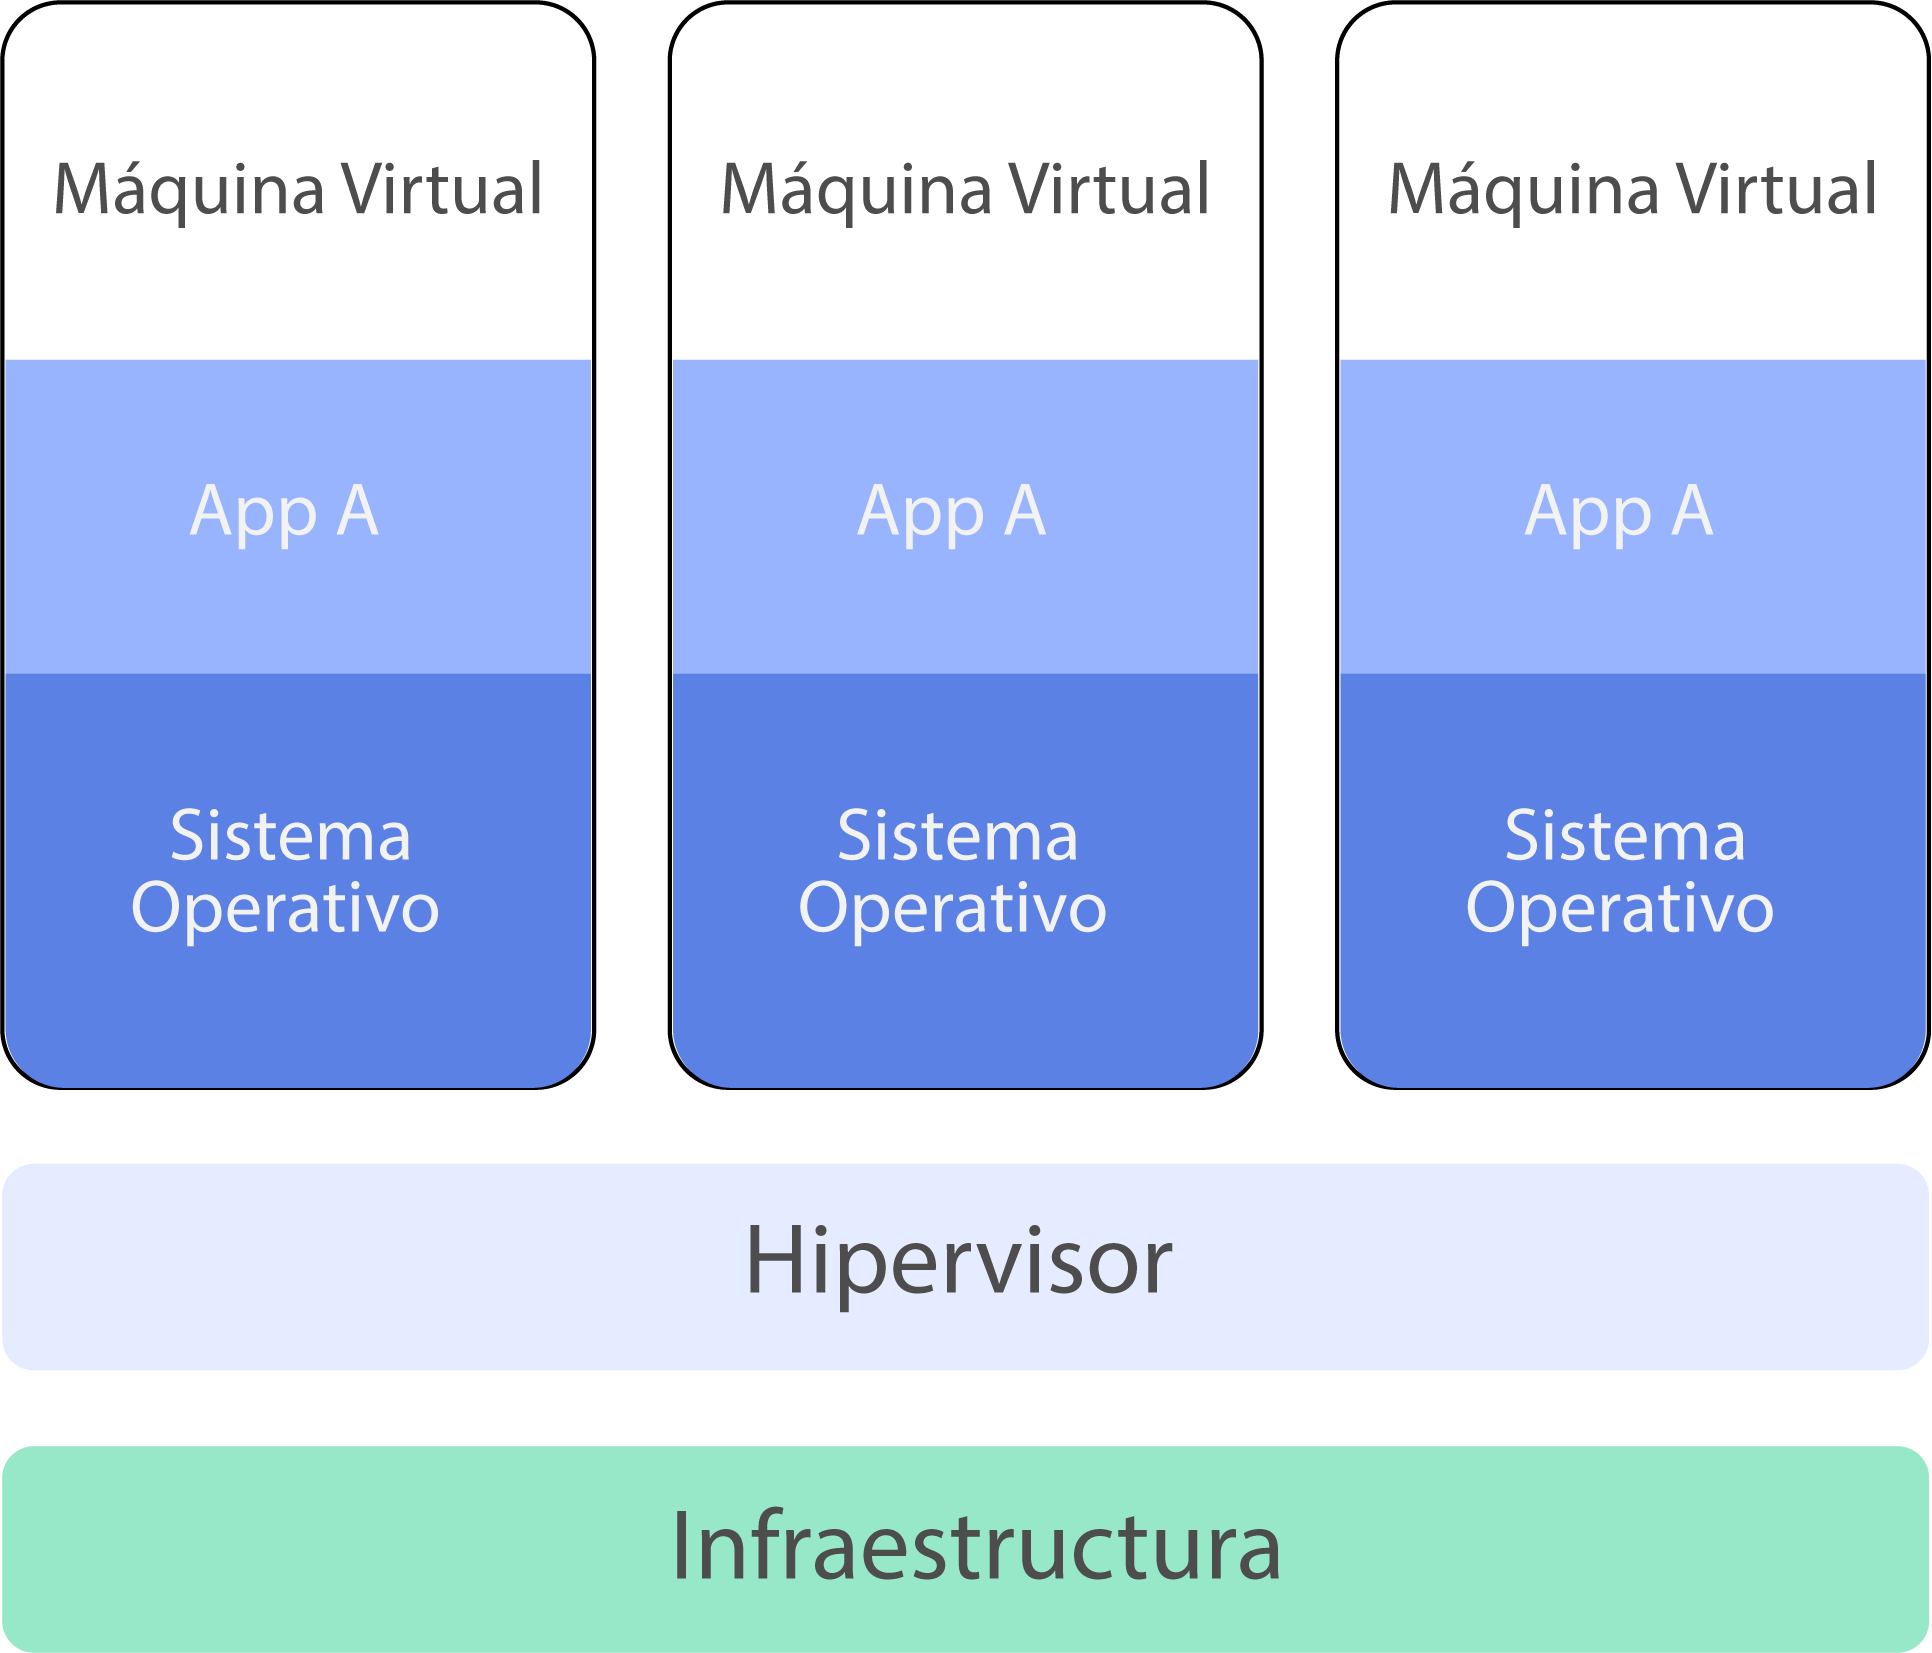
\includegraphics[scale=0.7]{images/vms.png}
  \captionof{figure}{Máquinas virtuales}
  \label{fig:vm}
\end{figure}

\break

Las máquinas virtuales (VMs) son una abstracción del hardware físico, transformando un servidor en múltiples servidores. El hypervisor permite que múltiples VMs corran en una misma máquina. Cada VM incluye una copia de un sistema operativo, la aplicación, los binarios y librerías, ocupando decenas de GBs.


\subsection[Docker Compose]{Docker Compose}

Docker Compose es una herramienta que permite correr un sistema formado por múltiples contenedores. Para ello, se debe crear un archivo .yml en el que se definan los servicios con los que va a contar la aplicación. Cada servicio estará formado por un contenedor corriendo una imágen de Docker. 
Para cada servicio pueden definirse nombres, puertos expuestos, conexiones de red, etc. Luego, con los siguientes comandos se puede operar con el sistema.

\section[Nginx]{Nginx}

Nginx es uno de los web servers más populares. Sirve tráfico HTTP y HTTPS, proxys a Python, NodeJS, corre software como balanceador de carga, http cache, SSL, etc.
Nginx es una pieza de software extremadamente modular. Muchas de las funcionalidades que trae por defecto, son en realidad módulos que se pueden activa y desactivar en cualquier momento. Una de las ventajas es que se puede decidir qué módulos se quiere utilizar, y cuales no.
Una de las funcionalidades más importantes para el desarrollo de microservicios es el proxy reverso.

\subsection[Forward proxy vs reverse proxy]{Forward proxy vs reverse proxy}

Una de las razones más populares para usar nginx es para que sirva aplicaciones dinámicas escritas en Python, NodeJS, Ruby, y muchas otras.
A diferencia de Apache, nginx no tiene la habilidad de embeber un intérprete al webserver, como hace Apache con mod\_php. En su lugar, nginx toma un enfoque mucho mas liviano. Es simplemente un webserver y su tarea principal es correr una aplicación web delegandolo a un server y proxies separados.

\subsection[Forward Proxy]{Forward Proxy}

Se le llama *forward proxy* a la configuración por defecto que se encuentra en todas las conexiones salientes de internet. Se ve algo asi:

\begin{figure}[h!]
  \centering
    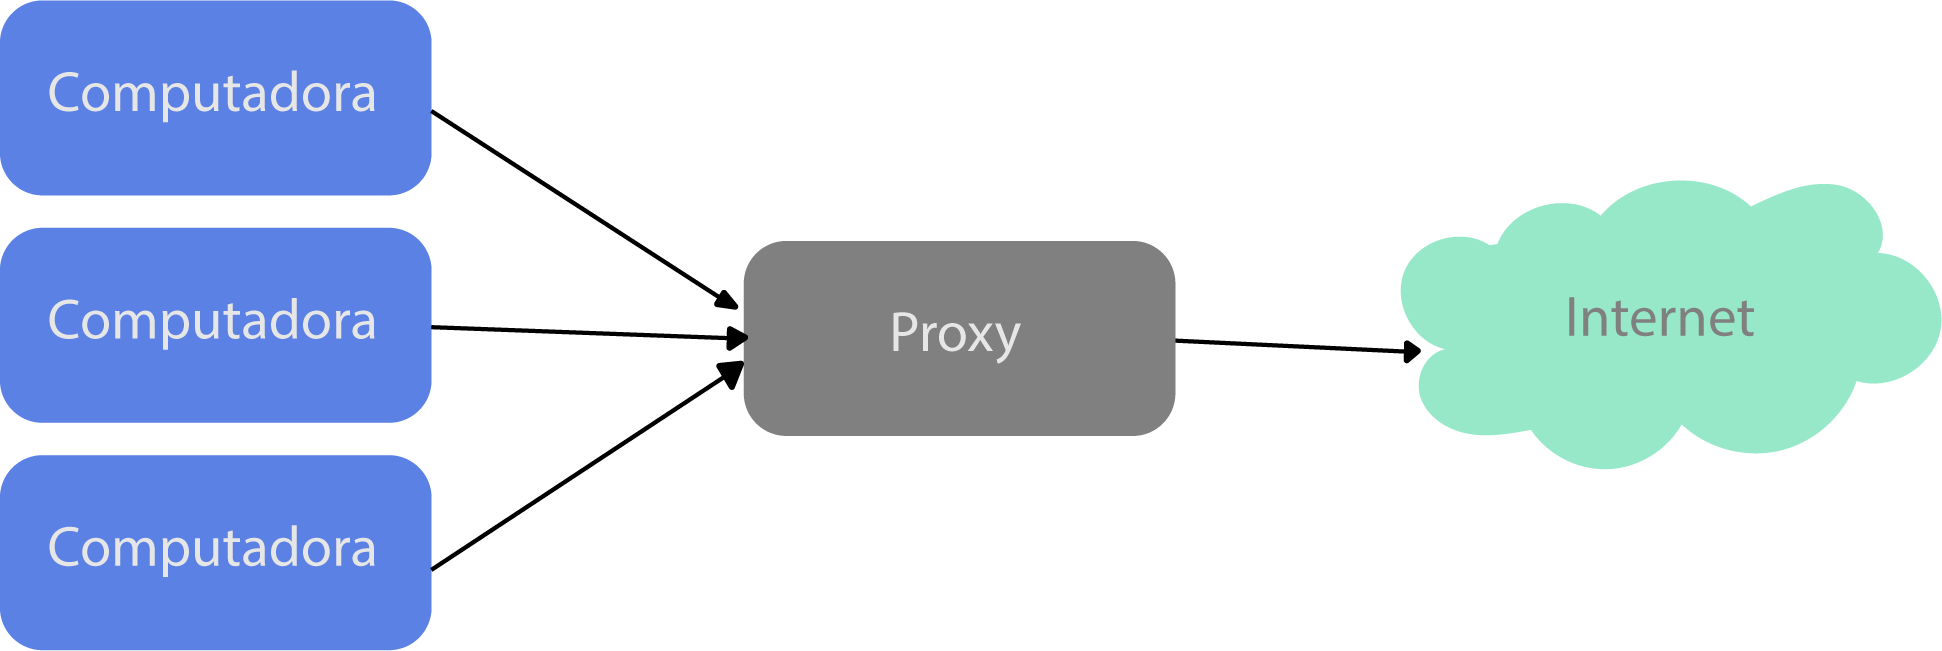
\includegraphics[scale=0.7]{images/forward-proxy.png}
  \captionof{figure}{Funcionamiento de Forward Proxy}
  \label{fig:forwardproxy}
\end{figure}

Las conexiones salientes de una computadora son capturadas por el *forward proxy* y reenviadas a Internet. Para Internet, todas las computadoras aparecen como si vinieran del mismo lugar- el *forward proxy*.


\subsection[Reverse Proxy]{Reverse Proxy}

Se le llama *reverse proxy* a lo opuesto de *forward proxy*, y es una configuración muy común para servir aplicaciones web dinámicas y para balance de carga.

\begin{figure}[h!]
  \centering
    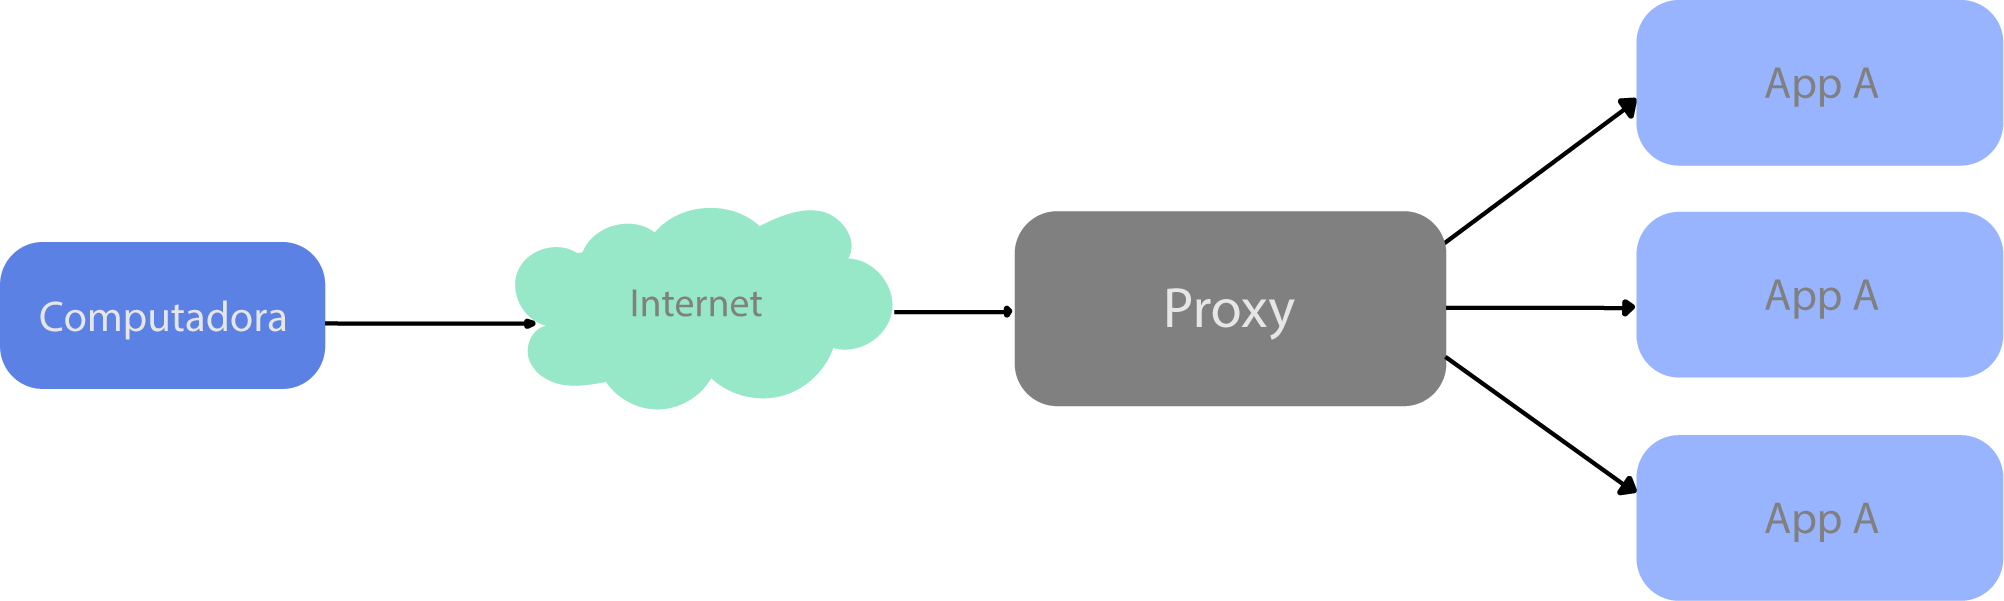
\includegraphics[scale=0.7]{images/reverse-proxy.png}
  \captionof{figure}{Funcionamiento de Reverse Proxy}
  \label{fig:reverseproxy}
\end{figure}

En este ejemplo, el *reverse proxy* hace de multiplexor para muchas conexiones de internet, a una aplicación dinámica. El *reverse proxy* mira el request, y lo reenvia a la aplicación.

\subsection[Balance de carga]{Balance de carga}

Una de las formas mas comunes de escalar una aplicación web es usar *balance de carga*. La idea detrás de esto, es distribuir la carga, o tráfico web, a través de diferentes *application servers*.
El funcionamiento normal de una sola aplicación con nginx es que los visitantes ingresan el nombre de dominio y son ruteados directamente al servidor donde nginx está sirviendo la *única* aplicación. El problema de esto es que cuando se tienen miles de conexiones visitando la aplicación, es probable que un solo servidor no pueda manejarlo. 
Ahi es cuando juega un papel importante el balanceador de carga, que recibe todo el tráfico ingresante y lo distribuye a través de un conjunto de servidores de aplicación.
Existen distintos tipos de balanceos de carga: por software y por hardware. Nginx tiene la habilidad de correr como un balanceador de carga de software, usando el módulo http_proxy.

El balance de carga es en definitiva un *reverse proxy*, con tres diferencias fundamentales: 
\begin{outline}
\1 Los balanceadores de carga reenvian el trafico a traves de varios *backends*, mientras que un reverse proxy tradicional lo hace hacia uno solo.
\1 Los balanceadores de carga usualmente operan en la capa 7 (HTTP) o en la capa 4 (TCP) del modelo OSI, cuando típicamente sólo operariamos en la capa 7 usando un *reverse proxy* de aplicaciones modernas.
\1 La escala es crítica para los balanceadores de carga: en sitios ocupados, pueden ver 20 veces la cantidad de tráfico que recibe un servidor de aplicación. Por ejemplo, un servidor de aplicaciones potente solo necesitará manejar entre 100 y 200 solicitudes por segundo, mientras que un balanceador de carga puede recibir más de 10,000 solicitudes por segundo.
\end{outline}
		\chapter{Desarrollo de la Solución}
\label{sec:desarrollo}

Las funcionalidades identificadas en los requerimientos del Capitulo 2 se implementaron en una aplicación llamada Seguimiento Académico usando la arquitectura y tecnologías descriptas en el Capitulo 3.
La aplicación Seguimiento Académico se conecta a una aplicación independiente que se encarga del análisis de los datos. Estos datos son obtenidos gracias a una tercer aplicación independiente llamada “Núcleo Académico”.
La Figura \ref{fig:analisis-nucleo} muestra el funcionamiento de estas tres aplicaciones.


\begin{figure}[H]
  \centering
    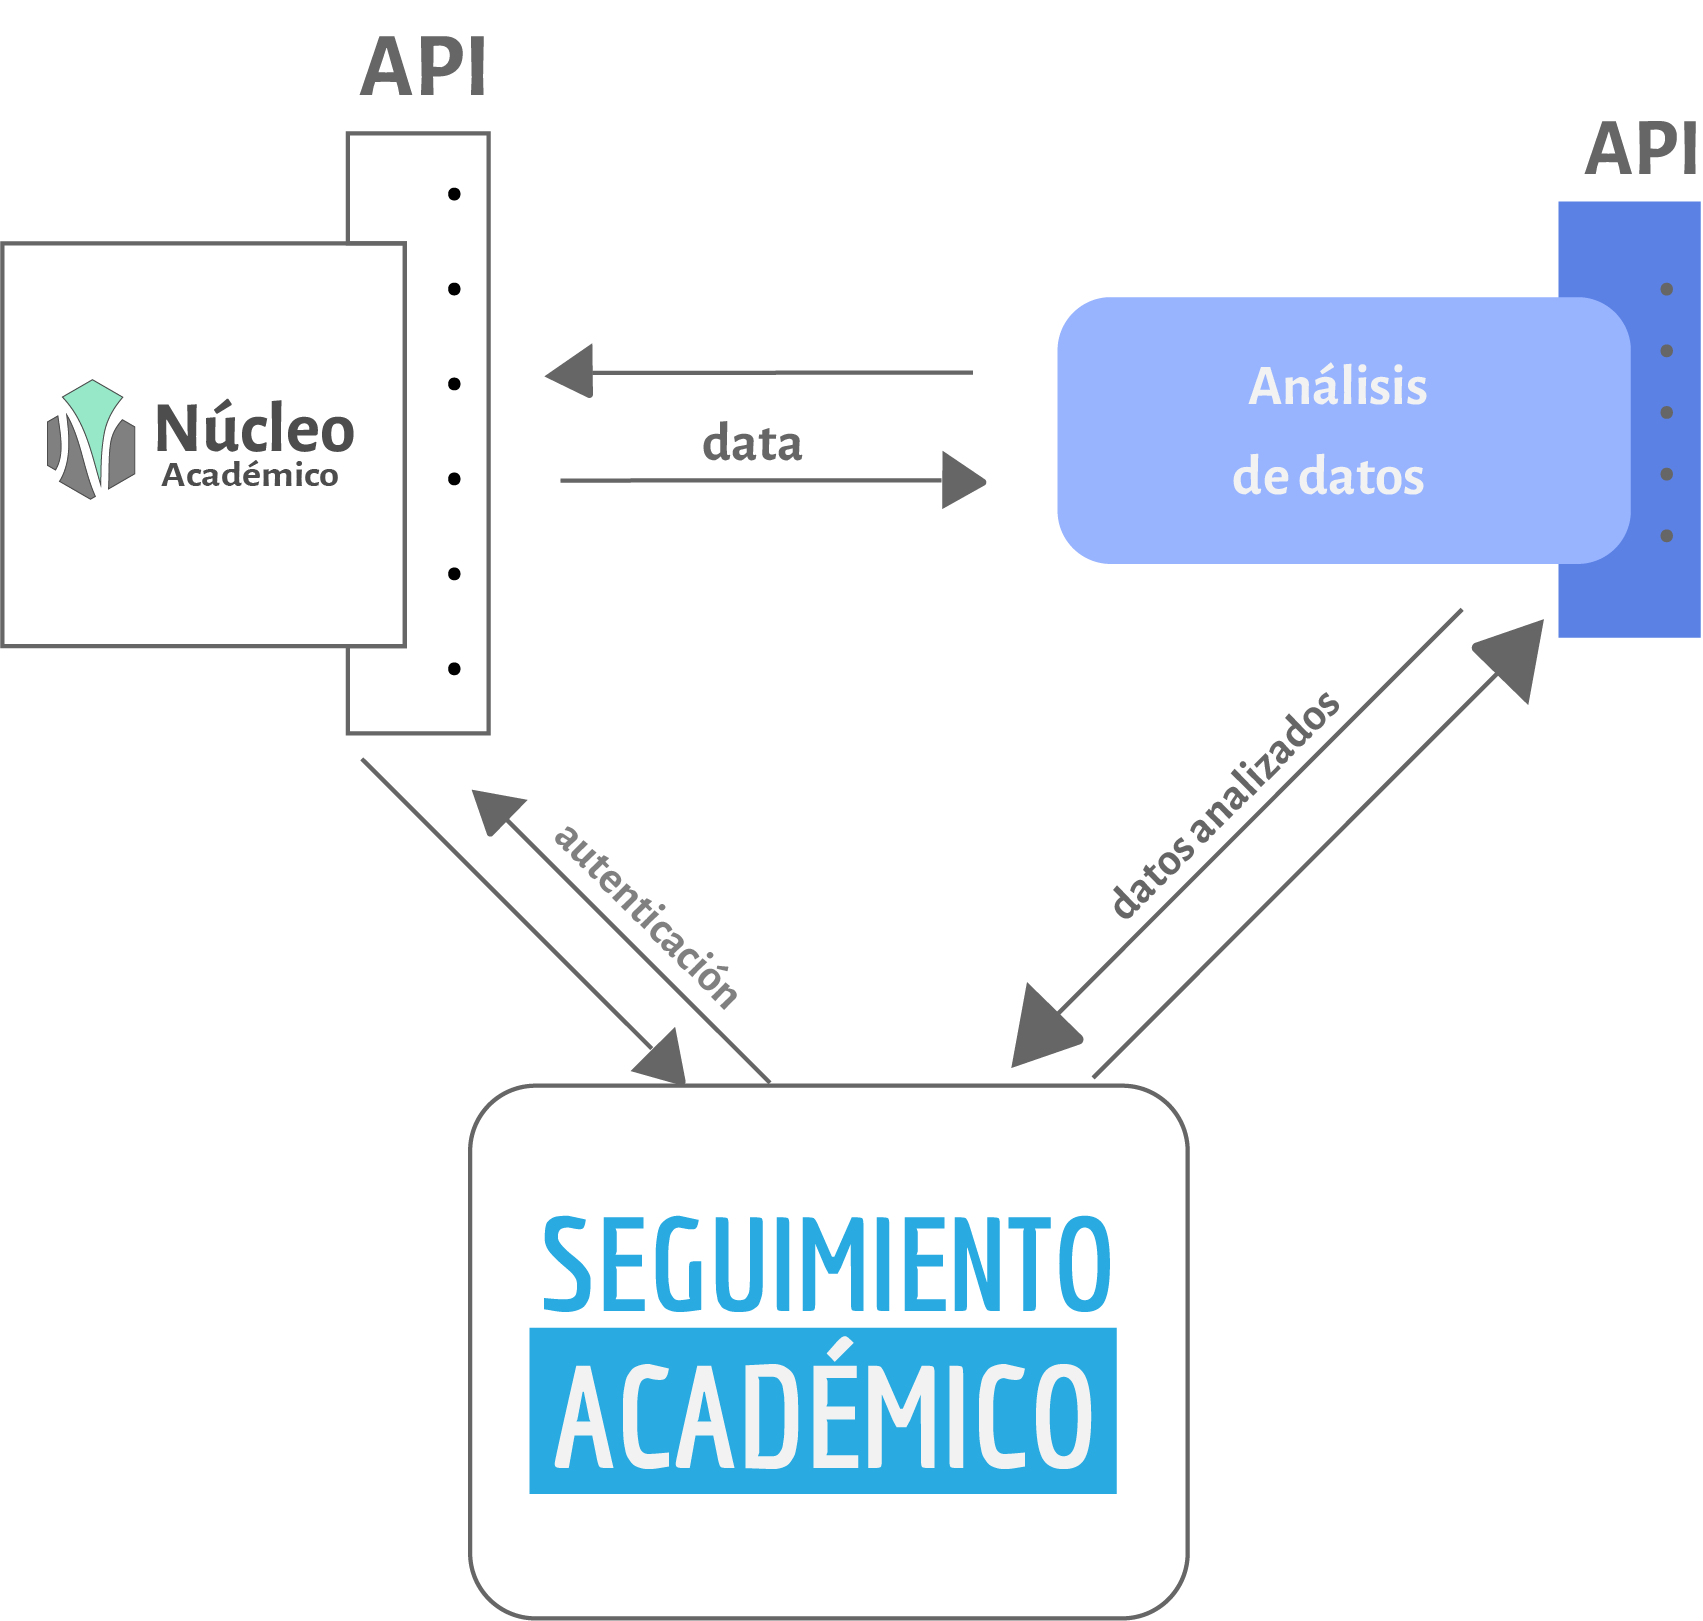
\includegraphics[scale=0.8]{images/seguimiento-academico/flow-seguimiento-academico.png}
  \captionof{figure}{Obtención de datos a través del núcleo}
  \label{fig:analisis-datos}
\end{figure}

Para el proceso de desarrollo de las aplicaciones se utilizó GIT como control de versiones del código y GitHub como repositorio del mismo. Además de usar GitHub como repositorio de código, se utilizó la herramienta de \textit{issues} para poder tener una mejor trazabilidad del código.

Adicionalmente se utilizó Travis para tener un entorno de integración continua. Esto significa que a medida que el desarrollo iba creciendo, esta herramienta se encargó de \textit{buildear} el código y correr los tests.  

\section[Núcleo]{Núcleo}

El núcleo se encarga de administrar los datos no sensibles de los estudiantes y sus materias cursadas, las inscripciones, planes de estudio con sus créditos, recorrido obligatorio y recomendado de inscripciones, entre otros.
El núcleo tiene la capacidad de servir dichos datos para que sean consumidos por los usuarios que tengan los permisos correspondientes.
Los usuarios tienen permisos asignados que corresponden con la carrera a la que pertenecen, que les permiten consultar datos de dicha carrera. 


\begin{figure}[h!]
  \centering
    
\includegraphics[scale=0.5]{images/nucleo/nucleo-fondoblanco.png}
  \captionof{figure}{Logo del Núcleo}
  \label{fig:django}
\end{figure}

\subsection{Tecnologías}

El Núcleo fue desarrollado con Python 3.6, usando el framework web Django en su versión 3.0.
Django incluye un administrador (django-admin) que genera automáticamente los listados, la creación, la edición y el borrado de los modelos desarrollados. Además, trae un sistema de autenticación de usuarios que facilita la tarea de autorizar usuarios a través de permisos.
Se eligió django-rest-framework para crear una API REST para que otros servicios puedan consultar o crear datos.
Usando django-rest-framework-simplejwt, se implementó JWT. Es decir, todo servicio que quiera acceder a los datos tendrá que pedir un token. Si éste está habilitado para consumir datos, se le proveerá de dicho token.

\subsection{Administración de los datos}

Los usuarios que tengan permiso para ingresar al Administrador, pueden hacerlo mediante una pantalla de Login como muestra la Figura ~\ref{fig:nucleo-login}.
Una vez ingresados, pueden ver la pantalla principal del administrador, como muestra la Figura ~\ref{fig:nucleo-home}, donde tienen diferentes menús para utilizar los datos. Tienen acceso a diferentes listados (Figura ~\ref{fig:nucleo-listado}), creación, edición y borrado (Figura ~\ref{fig:nucleo-edicion}).
Los usuarios tienen también la posibilidad de importar planillas de datos (Figura ~\ref{fig:nucleo-importador}).

\subsubsection{Usuarios y permisos}

Para resolver la autenticación y autorización en el administrador de contenidos, se usó el sistema de autenticación que viene embebido en Django.
Este sistema provee una manera de asignar permisos a usuarios específicos o grupos de usuarios. Estos permisos se dividen en:
\begin{outline}
    \1 El acceso a ver objetos está limitado a los usuarios que tengan los permisos \textit{view} o \textit{change}.
    \1 El acceso a ver los formularios para agregar elementos, está limitado a los usuarios que tengan el permiso \textit{add} para ese tipo de objetos.
    \1 El acceso a ver los listados, ver los formularios de edición y la posibilidad de editar, están limitados a los usuarios que tengan el permiso \textit{change} para ese objeto en particular.
    \1 El acceso a eliminar un objeto está limitado a los usuarios que tengan el permiso \textit{delete}.
\end{outline}

\subsubsection{Grupos de usuarios}

Django provee una forma de categorizar usuarios a los que se les puede aplicar permisos llamado \textit{grupo}. Un usuario puede pertenecer a muchos grupos.
Un usuario que pertenezca a un grupo, automáticamente tiene los permisos asignados a dicho grupo.
Otra particularidad de esto, además de los permisos, es que pueden servir para extender las funcionalidades. Por ejemplo, si quisiera que un grupo fuese “Usuarios de LIDS”, podría asignarle a ese grupo la carrera “LIDS” para que sólo pudieran ver datos relacionados a su carrera y no a otras.


\subsection{Importadores}

En el caso que los usuarios tengan la necesidad de importar los datos a través de planillas, se realizaron diferentes importadores para esta tarea (~\ref{fig:nucleo-importador}).
Estos importadores son:
\begin{outline}
\2 Carreras
\2 Planes de estudio con sus materias
\2 Prerrequisitos obligatorios y recomendados de materias
\2 Estudiantes con sus datos personales
\2 Materias cursadas por estudiantes
\2 Inscripciones a materias
\end{outline}

\subsection{API}

Se diseñó una API para consultar datos a través de distintas URIs (Tabla ~\ref{tab:tabla_api}), para las cuales se necesita de un token (Tabla ~\ref{tab:tabla_token}).
Dicho token es de la forma:

\textit{eyJ0eXAiOiJKV1QiLCJhbGciOiJIUzI1NiJ9.} \break 
\textit{eyJ0b2tlbl90eXBlIjoiYWNjZXNzIiwiZXhwIjoxNTg5Mjk2NjAyLCJ}\break 
\textit{qdGkiOiJhMTAzMmI2YzdiN2Y0ZjlkODc5NzI0NGViZTQxYTk5YSIsInV}\break 
\textit{zZXJfaWQiOjEsImNhcnJlcmFzIjpbIlciXSwiY2FycmVyYXNfbGFiZWwi} \break \textit{OltbIlciLCJMaWNlbmNpYXR1cmEgZW4gRGVzYXJyb2xsbyBkZSBTb2Z0d2}\break 
\textit{FyZSJdXSwidXNlcm5hbWUiOiJhZG1pbiJ9}.\break 
\textit{xWWi-sDFQ6I-CK0xC7tmkTw1mXRmMhFFse6\_qnKBiaE}

\break
El \textit{Header} del token tiene la siguiente información:
\begin{minted}[frame=single, framesep=3mm, linenos=true, xleftmargin=21pt, tabsize=4]{js}
{
"typ": "JWT",
"alg": "HS256"
}
\end{minted}
\break
Para el caso del \textit{Payload}, se tiene la siguiente información indicando precisamente qué carreras puede consultar el usuario:
\begin{minted}[frame=single, framesep=3mm, linenos=true, xleftmargin=21pt, tabsize=4]{js}
{
  "token_type": "access",
  "exp": 1589296602,
  "jti": "a1032b6c7b7f4f9d8797244ebe41a99a",
  "user_id": 1,
  "carreras": [
    "W"
  ],
  "username": "admin"
}
\end{minted}

\subsubsection{Ejemplo de pedido}
Si quisiera saber qué materias se definen dentro de una carrera en un plan determinado, debería hacer de la siguiente manera:

\begin{lstlisting}[language=bash]
GET 'https://url.del.nucleo/api/carreras/W/planes/2015/'
--header Authorization: Bearer <token>
\end{lstlisting}

El resultado tendrá la siguiente forma:

\begin{minted}[frame=single, framesep=3mm, linenos=true, xleftmargin=21pt, tabsize=4]{js}
[{
        "id": 54,
        "materia": "Taller de Trabajo Intelectual",
        "plan": 2015,
        "nucleo": "",
        "creditos": 4,
        "area": "Taller",
        "codigo": "00751"
    },
    ...
]
\end{minted}

La Figura~\ref{fig:nucleo-jwt} muestra al núcleo y un servicio que intenta hacer pedidos. Primero deberá enviar un pedido con sus credenciales para luego obtener un jwt. 
Una vez obtenido el jwt, puede hacer pedidos normalmente con el token en el header de cada request.

\begin{figure}[H]
  \centering
    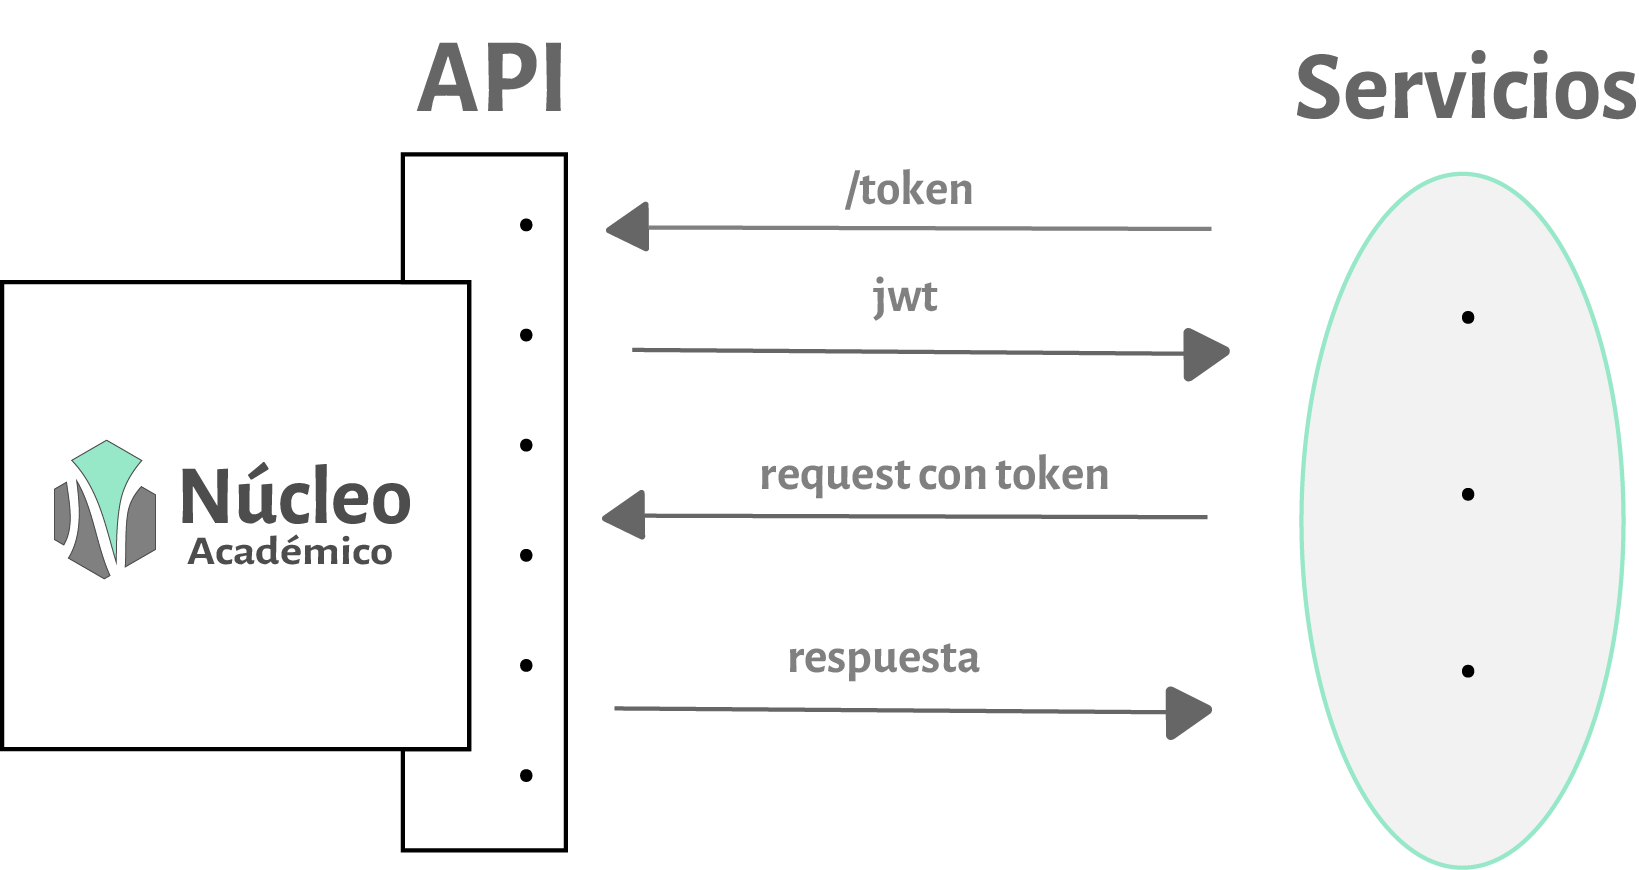
\includegraphics[scale=0.8]{images/nucleo/jwt.png}
  \captionof{figure}{Funcionamiento del pedido de token y posteriores requests}
  \label{fig:nucleo-jwt}
\end{figure}


\subsection{Deploy}

Para desplegar el núcleo se usa la siguiente configuración de docker-compose. Adicionalmente, se probaron configuraciones donde se disponen de varias instancias del núcleo limitando la cantidad de CPU y memoria de la que dispone cada uno. 

Esta es la configuración para una sola instancia, sin límite de CPU ni memoria.


\begin{minted}[gobble=4,frame=single,linenos]{yaml}
    
    # Se usa el formato 2.3 de docker-compose
    version: '2.3'
    # Defino los servicios a utilizar
    services:
      # En este caso, se muestra con una sola instancia
      nucleo-academico_1:
        # Defino el nombre del contenedor
        container_name: nucleo-academico_1
        # Siempre debe reiniciarse
        restart: always
        # El contexto de build es el directorio actual
        build: .
        # Defino el comando para iniciar la aplicación
        command: gunicorn -w 1 -b :8001 alumnos.wsgi:application
        # Defino los volúmenes
        volumes:
          - .:/code
        # Esta instancia va a estar corriendo en el puerto 8001
        ports:
          - "8001:8001"
        # Defino el archivo de configuraciones del entorno
        env_file:
          - ./.env
      # Pongo a nginx como otro servicio
      nginx:
        # Seteo el nombre del contenedor
        container_name: nginx-container
        restart: always
        build: ./nginx
        # Nginx va a correr en el puerto 8000 dentro del contenedor 
        # y hago un mapeo al 80 local
        ports:
          - "8000:80"
        # Le informo que va a depender del nucleo-academico_1
        depends_on:
          - nucleo-academico_1
    
    # Defino las networks, que serviran para conectar los contenedores
    networks:
      default:
        external:
          name: seguimiento-academico
  \end{minted}

\section[Análisis de Datos]{Análisis de Datos}

Para poder obtener información relevante de las carreras, materias y estudiantes, se debe hacer un análisis de los datos recopilados históricamente.

Si bien el núcleo provee una gran cantidad de datos, éstos necesitan una manipulación, procesamiento y una limpieza para que puedan ser analizados.

El objetivo principal de este módulo es de la obtención de los datos mediante una API Rest, la manipulación y el procesamiento de esos datos. Una vez terminado este proceso, sirve los resultados mediante una API Rest, que es consumida por un tercero para su visualización.

\subsection{Especificaciones}

El módulo de análisis de datos está construido con Python 3.6. El análisis de los datos se hizo con Pandas y los resultados son servidos gracias a Flask a través de una API REST.


La Figura ~\ref{fig:analisis-nucleo} muestra el rol de este módulo y su funcionamiento con respecto al núcleo

\begin{figure}[h!]
  \centering
    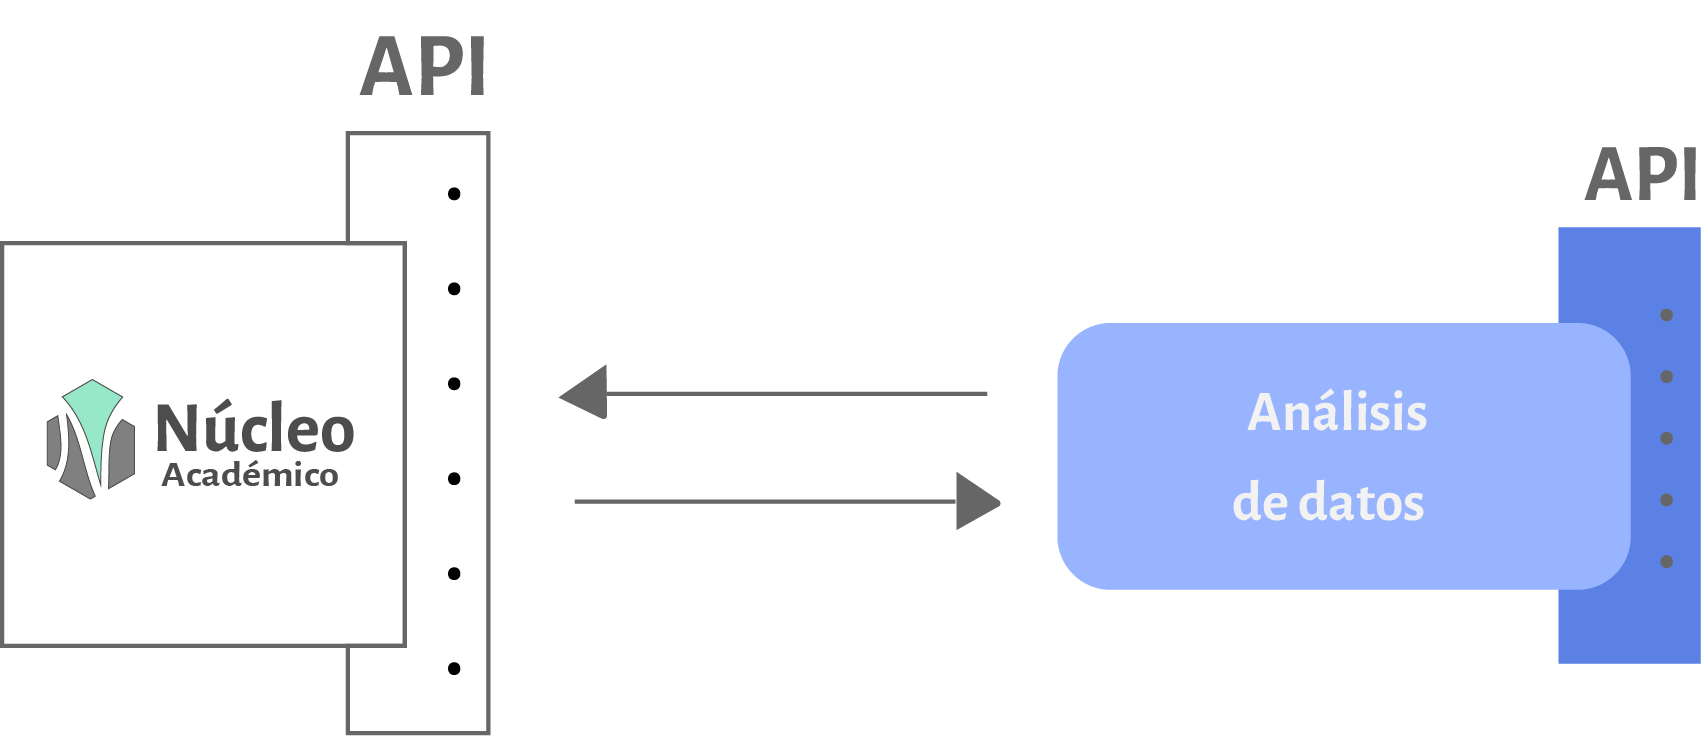
\includegraphics[scale=0.8]{images/analisis-datos/analisis-datos.png}
  \captionof{figure}{Obtención de datos a través del núcleo}
  \label{fig:analisis-nucleo}
\end{figure}


\subsection{Obtención de los datos}

Los datos son obtenidos a través de pedidos a la API del Núcleo. Estos datos llegan en forma de JSON y son transformados a DataFrame o Series (estructuras de datos de Pandas). 

Dado que los datos llegan de forma de recursos independientes, la mayor parte de los análisis requieren que estos datos sean unidos gracias a las funcionalidades de los DataFrames (de forma similar a los join de SQL).

\subsection{Análisis}

Una vez terminados los procesos de obtención, limpiado y union de los datos, se empieza el proceso de análisis.

Se realizaron análisis de diferentes magnitudes, basado en la cantidad de procesamiento que requieren. 
\subsubsection{Análisis sobre materias}

\paragraph{Datos basicos históricos} \mbox{}\\

URI: /materias/<cod\_materia>/basicos \\

Parámetros opcionales: inicio: yyyy-mm-dd, fin: yyyy-mm-dd, carrera: código de la carrera. \\

Dada una materia, analiza cuántos estudiantes aprobaron, cuántos estudiantes desaprobaron, cuántos estudiantes quedaron ausentes y cuántos estudiantes faltan aprobarla dentro de un período de tiempo.

\paragraph{Detalle de aprobación}\mbox{}\\

URI: /materias/<cod\_materia>/detalle-aprobados \\

Parámetros opcionales: inicio: yyyy-mm-dd, fin: yyyy-mm-dd, carrera: código de la carrera. \\

Dada una materia, informa el detalle de estudiantes aprobados, teniendo en cuenta la forma de aprobación. Las formas de aprobacion son:

\begin{outline}
    \2 Equivalencia equivalente
    \2 Promoción en otra carrera
    \2 Promoción
    \2 Equivalencia
    \2 Examen equivalente
    \2 Examen
\end{outline}

\paragraph{Dispersión de notas}\mbox{}\\

URI: /materias/<cod\_materia>/dispersion-notas \\

Parámetros opcionales: inicio: yyyy-mm-dd, fin: yyyy-mm-dd, carrera: código de la carrera. \\

Dada una materia, se hace un análisis de la dispersión de las notas dentro de un período. Teniendo en cuenta estudiantes, sus notas y el promedio de ese estudiante.

\paragraph{Número de recursantes}\mbox{}\\

URI: /materias/<cod\_materia>/recursantes \\

Parámetros opcionales: inicio: yyyy-mm-dd, fin: yyyy-mm-dd, carrera: código de la carrera. \\

Dada una materia, analiza qué estudiantes son recursantes y cuantas veces.


\subsubsection{Análisis sobre estudiantes}

\paragraph{Porcentaje de aprobación por área}\mbox{}\\

URI: /alumnos/<legajo>/porcentajes-areas \\

Parámetros adicionales: carrera, inicio, fin, plan \\

Dado un estudiante, se hace un análisis de los porcentajes de aprobación que tiene con respecto a las diferentes áreas de la carrera y el plan que se está analizando, dentro del período elegido.

Cada carrera tiene sus propias áreas. En particular, y tomado a forma de ejemplo, las áreas de la Licenciatura en Informática se muestran en la Tabla ~\ref{tab:tabla_areas}.

\begin{table}[!htbp]
    \centering
    \makegapedcells
    \begin{tabular}{|c|c|}
    \hline
    Nombre \\ \hline
    Programación \\ \hline
    Sistemas Informáticos \\ \hline
    Procesos Informáticos\\ \hline
    Desarrollo de Software \\ \hline
    Teoría de la Computación \\ \hline
    \end{tabular}
    \caption{Áreas de la Licenciatura en Informática}
    \label{tab:tabla_areas}
\end{table}

\paragraph{Porcentaje de aprobación por núcleo}\mbox{}\\

URI: /alumnos/<legajo>/porcentajes-nucleos \\

Parámetros adicionales: carrera, inicio, fin, plan \\

Dado un estudiante, se hace un análisis de los porcentajes de aprobación que tiene con respecto a los diferentes núcleos de la carrera y el plan que se está analizando, dentro del período elegido.

Cada carrera tiene sus propios núcleos. En particular, y tomado a forma de ejemplo, los núcleos de la Licenciatura en Informática se muestran en la Tabla ~\ref{tab:tabla_nucleos}.

\begin{table}[!htbp]
    \centering
    \makegapedcells
    \begin{tabular}{|c|c|}
    \hline
    Código & Nombre \\ \hline
    I & Introductorio \\ \hline
    B & Básico\\ \hline
    A & Avanzado \\ \hline
    C & Complementario/Orientativo \\ \hline
    \end{tabular}
    \caption{Núcleos de la Licenciatura en Informática}
    \label{tab:tabla_nucleos}
\end{table}


\paragraph{Notas}\mbox{}\\

URI: /alumnos/<legajo>/notas \\

Parámetros adicionales: carrera, inicio, fin, plan \\

Dado un estudiante, se obtienen las diferentes notas que tuvo a lo largo de sus cursadas.

\paragraph{Porcentaje de avance de carrera}\mbox{}\\

URI: /alumnos/<legajo>/porcentaje-carrera \\

Parámetros adicionales: carrera, inicio, fin, plan \\

Dado un legajo de estudiante, se realiza un análisis para determinar el porcentaje de avance de la carrera, según el plan que se analice. Dado que cada plan tiene una cantidad distinta de materias, este dato cambia según el plan que se analice.

\paragraph{Promedio por períodos}\mbox{}\\

URI: /alumnos/<legajo>/scores \\

Parámetros adicionales: carrera, inicio, fin, plan \\

Dado un estudiante, se calcula cuál fue su \textit{score} por cada período. Es decir, su rendimiento semestral. 

El \textit{score} se calcula sacando un promedio de sus notas en un semestre. Las materias que sólo se distinguen entre “Aprobado” y “Desaprobado” y no disponen de una nota, se les asigna una nota para sacar este promedio.
Las materias con nota “Aprobado” son consideradas como un 7, y las materias con nota “Desaprobado” son consideradas como un 3. Entonces, el \textit{score} no es un promedio preciso, sino una estipulación de lo que fué su rendimiento en ese período.

Este \textit{score} es útil para analizar el rendimiento de un estudiante y puede servirle a las carreras para tomar decisiones tempranas.

\subsubsection{Análisis sobre carreras}

\paragraph{Cantidad de estudiantes por semestre}\mbox{}\\

URI: /carreras/<carrera>/alumnos \\

Dada una carrera, se obtiene un listado de cantidad de inscriptos por semestre


\paragraph{Datos generales por cohorte}\mbox{}\\

URI: /carreras/<carrera>/cantidades-alumnos \\

Dada una carrera, se obtiene un listado de inscriptos, cursantes, graduados y postulantes por cohorte.


\paragraph{Ingresantes por cohorte}\mbox{}\\

URI: /carreras/<carrera>/cantidades-ingresantes \\

Dada una carrera, se obtiene la cantidad de ingresantes separadas por año.


\paragraph{Cantidad de cursantes actual}\mbox{}\\

URI: /carreras/<carrera>/cursantes-actual \\

Dada una carrera, se obtiene la cantidad de cursantes actual.


\paragraph{Cantidad de ingresantes actual}\mbox{}\\

URI: /carreras/<carrera>/ingresantes-actual \\

Dada una carrera, se obtiene la cantidad de ingresantes.


\paragraph{Cantidad total de graduados} \mbox{}\\

URI: /carreras/<carrera>/graduados-total \\

Dada una carrera, se obtiene el total de graduados.


\paragraph{Dispersión de scores y promedios}\mbox{}\\
URI: /carreras/<carrera>/dispersion-score-promedio \\

El objetivo de este análisis es el agrupar estudiantes en base al \textit{score} y al promedio. Mostrando grupos de interés sobre los cuales se podrán implementar acciones específicas.

\paragraph{Materias que demoran la formación}\mbox{}\\

URI: /carreras/<carrera>/materias-traba \\

Dada una carrera, se quiere analizar qué materias son las que demoran la formación de los estudiantes. 
Para poder realizar este análisis, se necesitaron los siguientes datos:
\begin{outline}
\1 Índice de aprobación de una materia (cantidad de aprobados / cantidad total de cursantes).
\1 Cuántas materias obligatorias dependen de ella.
\end{outline}

Luego de calcular estos datos materia por materia, se calcula un \textit{score}. Este \textit{score} determina qué materia puede llegar a demorar la carrera de un estudiante.

\begin{align*}
  Score = (1 - IndiceAprobacion) * CantidadObligatoriasDependientes\\
\end{align*}

Es decir, que una materia que tiene un porcentaje de aprobación del 75\% y 10 materias que son obligatorias y dependen de ésta para ser cursadas, tendrá un score de 2.5 ((1 - 0.75) * 10).



\section[Visualización de los datos analizados]{Visualización de los datos analizados}

Si bien la parte de análisis de datos quedó cubierta, era necesario poder visualizarlos de forma gráfica. Por esta razón surgió la necesidad de crear una nueva aplicación independiente del núcleo y del análisis de datos.

Esta nueva aplicación obtuvo el nombre de Seguimiento Académico, y su logo se muestra en la Figura ~\ref{fig:seguimiento-academico-logo}.

\begin{figure}[h!]
  \centering
    
\includegraphics[scale=0.5]{images/seguimiento-academico/seguimiento-academico-blanco.png}
  \captionof{figure}{Logo de la aplicación de Seguimiento Académico}
  \label{fig:seguimiento-academico-logo}
\end{figure}

Su objetivo principal es recolectar los datos analizados y mostrarlos de forma gráfica, dependiendo de los permisos que tenga el usuario que realiza el pedido.
Estos datos se desprenden del módulo de análisis, y se agrupan de la siguiente manera:

\begin{outline}
\2 Datos sobre carreras.
\2 Datos sobre materias.
\2 Datos sobre estudiantes.
\end{outline}

Cada uno de estos grupos de datos tiene su propia pantalla de tipo reporte, donde el usuario ingresa los parámetros necesarios para cada reporte.


\subsection{Especificaciones}

Seguimiento Académico está construido con React 16.8 y se usó la biblioteca recharts para generar gráficos. Además, se uso el framework Material UI para el renderizado de elementos de la interfáz de usuario y diferentes tablas.
Este módulo realiza pedidos a la aplicación de análisis de datos, los cuales tienen que tener su correspondiente token para ser aceptados.
Cuando un usuario ingresa, se hace una autenticación con el núcleo. Esta autenticación tiene como resultado un token, y éste será utilizado para realizar todos los pedidos de datos correspondientes.


El gráfico ~\ref{fig:analisis-datos} muestra el rol de este módulo y su funcionamiento con respecto al de análisis de datos y al núcleo.

\subsection{Obtención de los datos}

Los datos son obtenidos a través de pedidos a la API del módulo de análisis de datos gracias a Axios.
Axios está basado en \textit{promises}, con lo cual se puede aprovechar las ventajas de \textit{async} y \textit{await} para un código asincrónico más legible.

Estos pedidos se realizan a través de llamadas \textit{ajax}, lo cual quiere decir que la página carga normalmente y realiza los pedidos de forma asincrónica e independiente entre los gráficos. A medida que los datos van llegando, cada gráfico se va \textit{renderizando}.

Estos datos llegan como JSON y son procesados para ser mostrados de forma correcta.


\subsection{Visualización de datos}

La aplicación Seguimiento Académico tiene 5 pantallas principales:
\begin{outline}
 \1 Login (Figura ~\ref{fig:sa-login}).
 \1 Home (Figura ~\ref{fig:sa-home})
 \1 Reporte de Carrera (Figura ~\ref{fig:sa-carrera})
 \1 Reporte de Materia (Figura ~\ref{fig:sa-materia})
 \1 Reporte de Alumno (Figura ~\ref{fig:sa-alumno})
\end{outline}


\begin{figure}[!htbp]
  \centering
    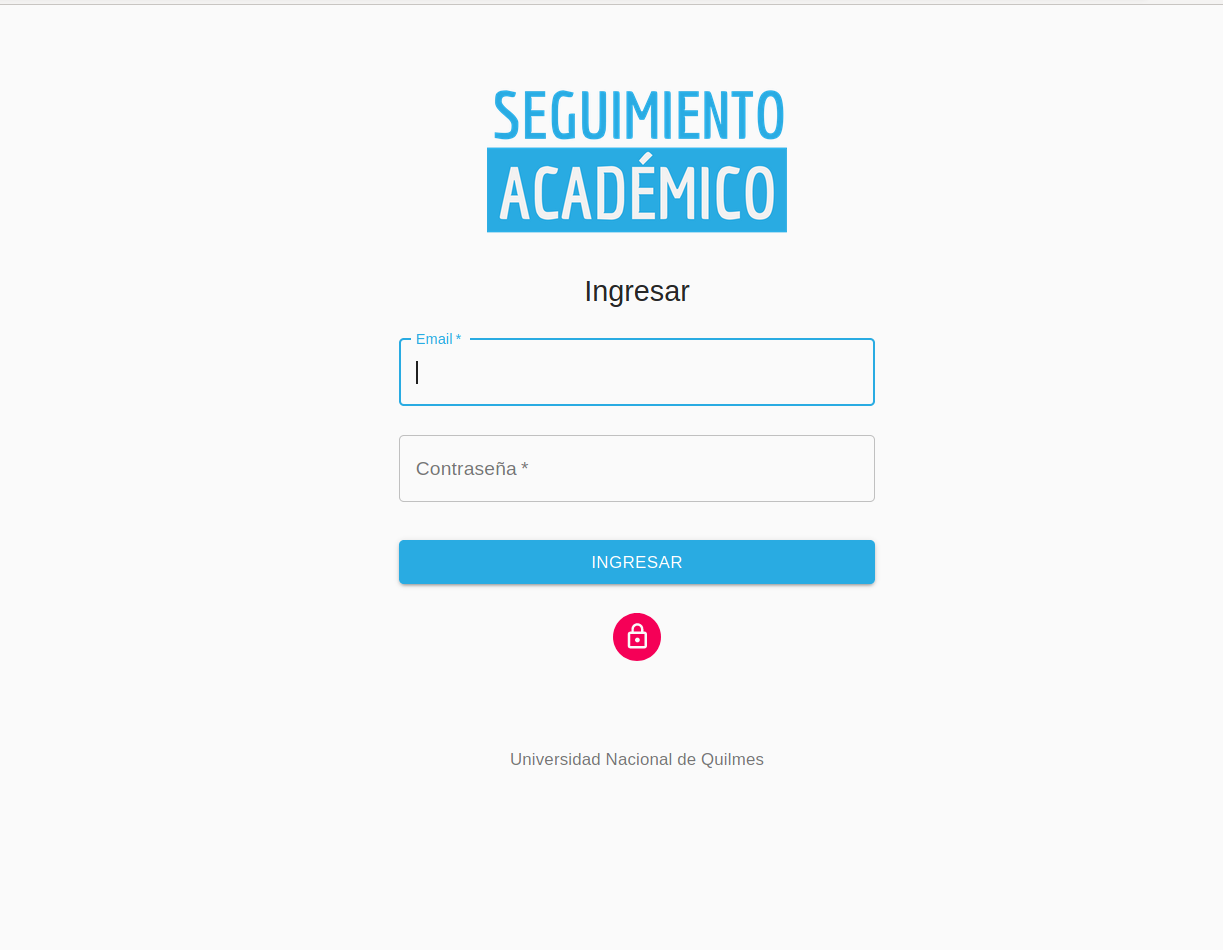
\includegraphics[scale=0.3]{images/seguimiento-academico/sa-login.png}
  \captionof{figure}{Login de Seguimiento Académico}
  \label{fig:sa-login}
\end{figure}

\begin{figure}[!htbp]
  \centering
    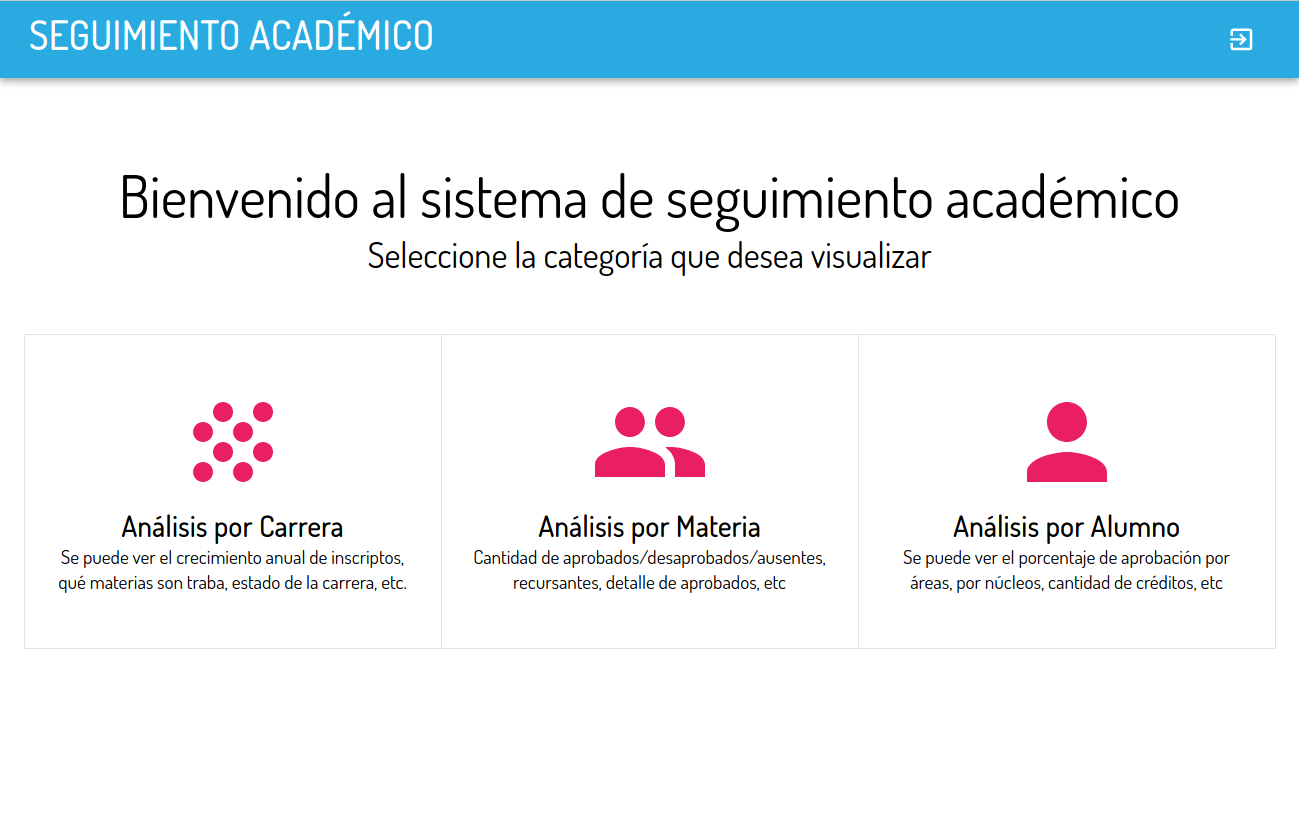
\includegraphics[scale=0.3]{images/seguimiento-academico/sa-home.png}
  \captionof{figure}{Pantalla principal de Seguimiento Académico}
  \label{fig:sa-home}
\end{figure}

\begin{figure}[!htbp]
  \centering
    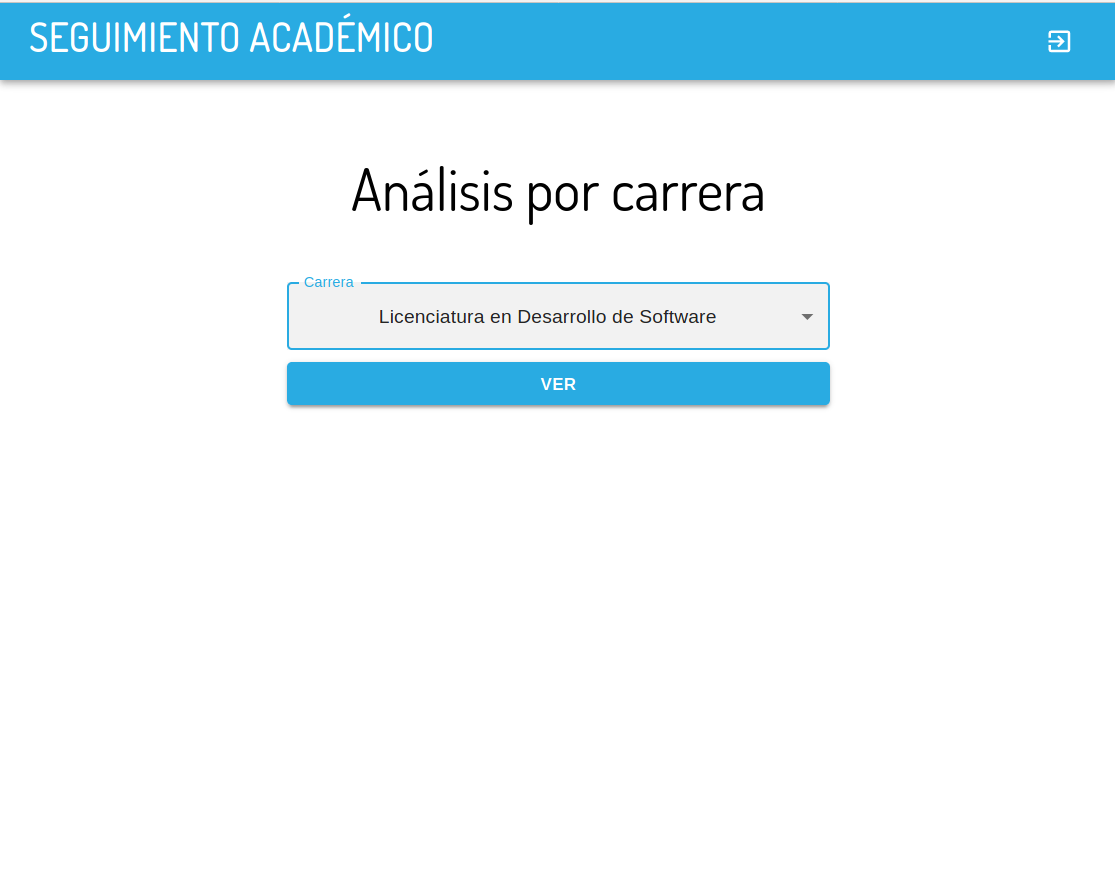
\includegraphics[scale=0.3]{images/seguimiento-academico/sa-form-carrera.png}
  \captionof{figure}{Pantalla Reporte de Carrera de Seguimiento Académico}
  \label{fig:sa-carrera}
\end{figure}

\begin{figure}[!htbp]
  \centering
    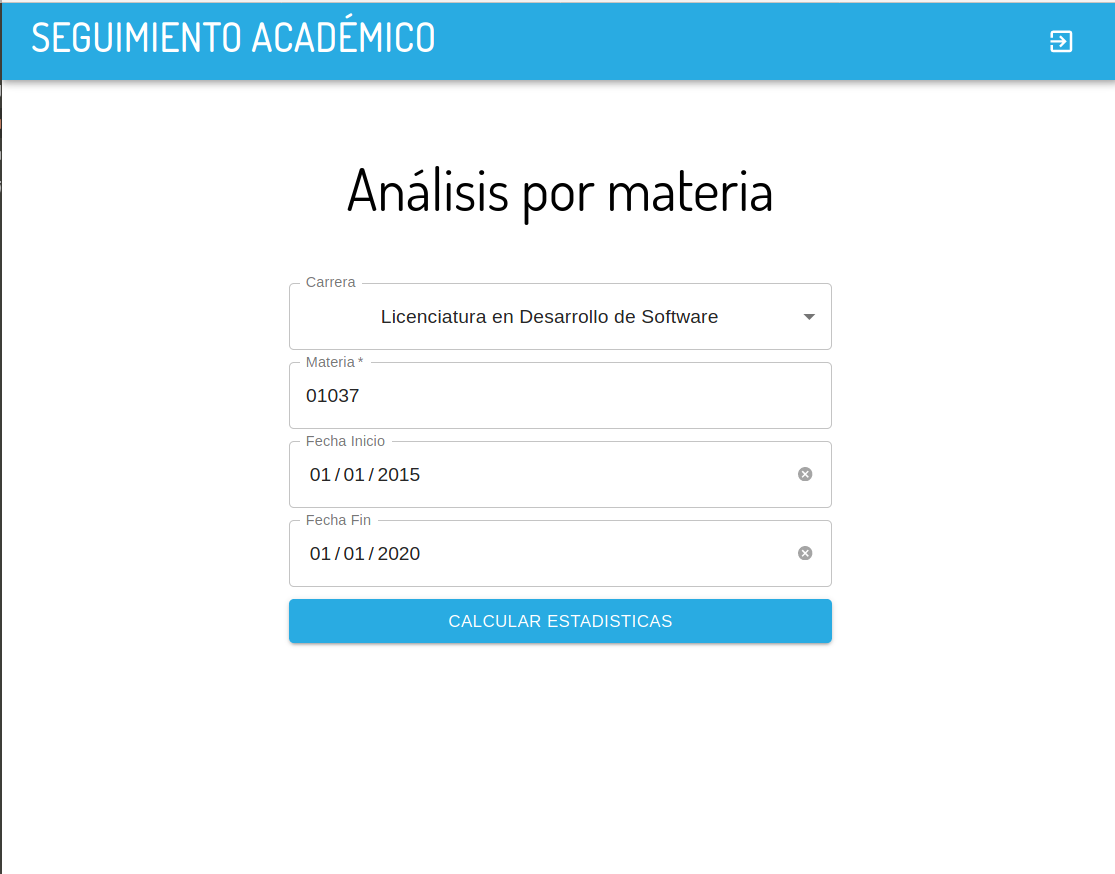
\includegraphics[scale=0.3]{images/seguimiento-academico/sa-form-materia.png}
  \captionof{figure}{Pantalla Reporte de Materia de Seguimiento Académico}
  \label{fig:sa-materia}
\end{figure}

\begin{figure}[!htbp]
  \centering
    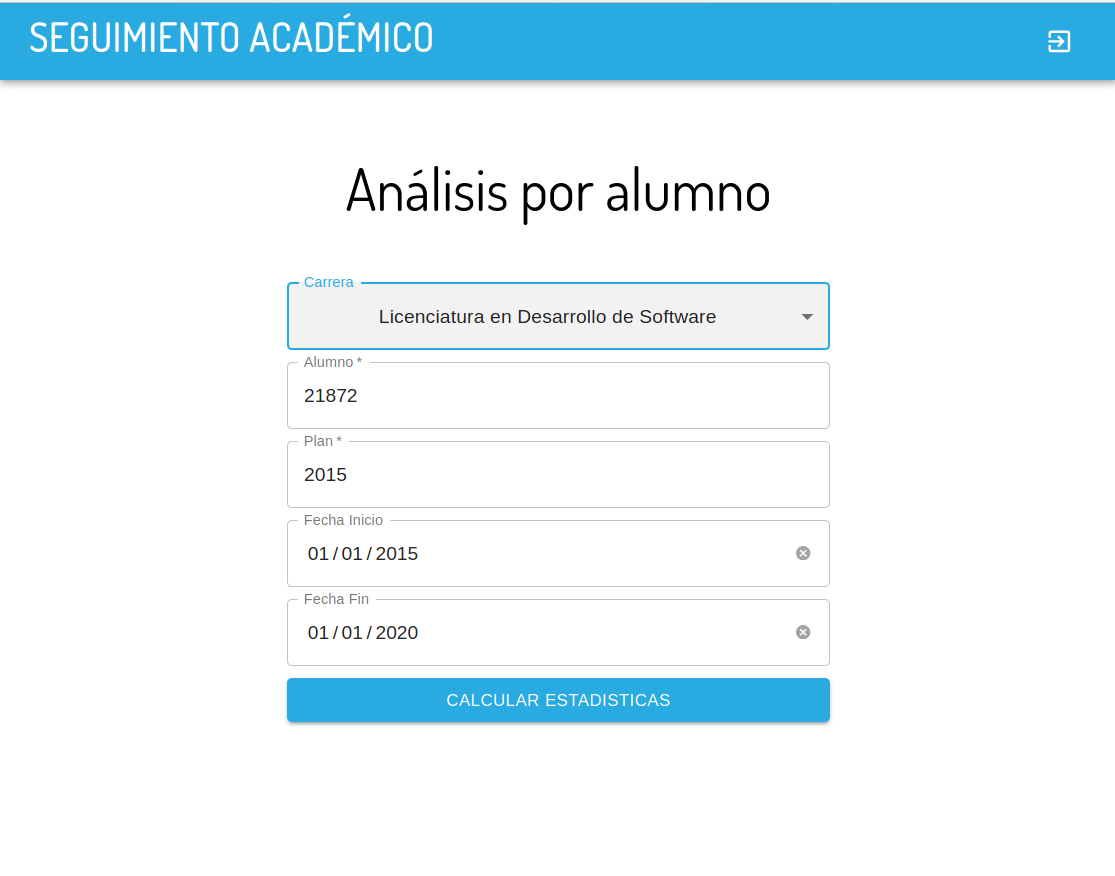
\includegraphics[scale=0.3]{images/seguimiento-academico/sa-form-alumno.png}
  \captionof{figure}{Pantalla Reporte de Alumno de Seguimiento Académico}
  \label{fig:sa-alumno}
\end{figure}


\subsubsection{Visualización por carrera}

Se dispone de un formulario para realizar un reporte, donde el usuario puede seleccionar entre sus carreras disponibles. Una vez que el formulario fue completado, se muestran los siguientes gráficos.

\paragraph{Cantidad actual de cursantes} \mbox{}\\
La cantidad actual de cursantes de la carrera se muestra en forma de tarjeta informativa (Figura~\ref{fig:sa-cursantes}). 

\begin{figure}[H]
  \centering
    
\includegraphics[scale=0.4]{images/seguimiento-academico/sa-cursantes.png}
  \captionof{figure}{Cantidad de cursantes}
  \label{fig:sa-cursantes}
\end{figure}

\paragraph{Cantidad actual de ingresantes} \mbox{}\\
La cantidad actual de ingresantes de la carrera se muestra en forma de tarjeta informativa (Figura~\ref{fig:sa-ingresantes}).

\begin{figure}[H]
  \centering
    
\includegraphics[scale=0.4]{images/seguimiento-academico/sa-ingresantes.png}
  \captionof{figure}{Cantidad de ingresantes}
  \label{fig:sa-ingresantes}
\end{figure}

\paragraph{Cantidad total de graduados} \mbox{}\\
La cantidad total de graduados de la carrera se muestra en forma de tarjeta informativa (Figura~\ref{fig:sa-graduados}).

\begin{figure}[H]
  \centering
    
\includegraphics[scale=0.4]{images/seguimiento-academico/sa-graduados.png}
  \captionof{figure}{Cantidad de graduados}
  \label{fig:sa-graduados}
\end{figure}

\paragraph{Dispersión de estudiantes} \mbox{}\\
El siguiente gráfico muestra la dispersión de los estudiantes con respecto a su promedio general y su desempeño el último año. Uno de los ejes tiene en cuenta el promedio y el otro su score el último año. De esta manera, se puede observar de forma gráfica los estudiantes que se desempeñaron por encima de su historial y cuáles no (Figura~\ref{fig:sa-dispersion}).

\begin{figure}[H]
  \centering
    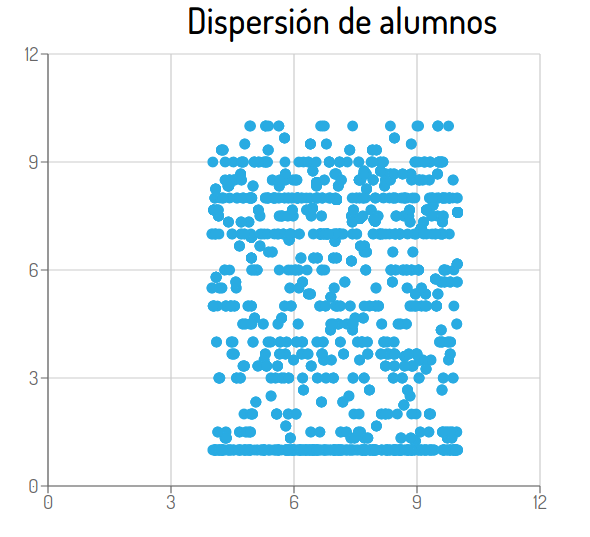
\includegraphics[scale=0.4]{images/seguimiento-academico/sa-dispersion.png}
  \captionof{figure}{Gráfico de dispersión}
  \label{fig:sa-dispersion}
\end{figure}

\paragraph{Cantidad de ingresos por semestre} \mbox{}\\
El siguiente gráfico es en forma de \textit{área}, y muestra la cantidad de ingresos semestrales histórico de la carrera. De esta forma, se puede observar en qué momento hubo picos de ingresos y en qué momentos hubo menos (Figura~\ref{fig:sa-ingresos-semestre}).

\begin{figure}[H]
  \centering
    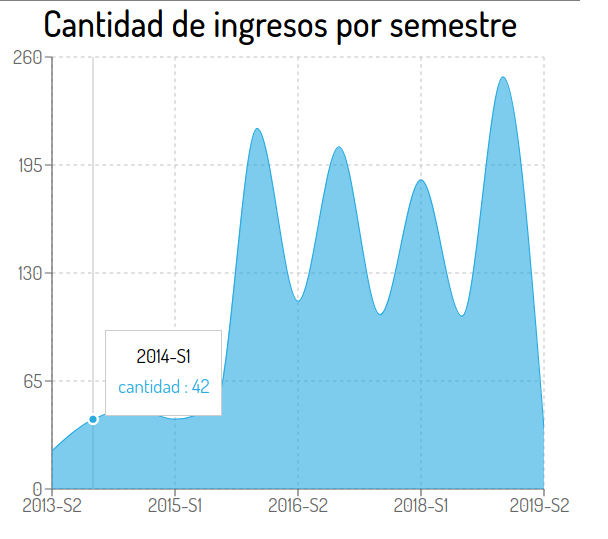
\includegraphics[scale=0.4]{images/seguimiento-academico/sa-ingresossemestre.png}
  \captionof{figure}{Ingresos por semestre}
  \label{fig:sa-ingresos-semestre}
\end{figure}

\paragraph{Alumnos por cohorte} \mbox{}\\
La siguiente es una tabla que detalla año a año de la carrera, qué cantidad de cursantes hubo, la cantidad de ingresantes y la cantidad de graduados  (Figura~\ref{fig:sa-alumnos-cohorte}).

\begin{figure}[H]
  \centering
    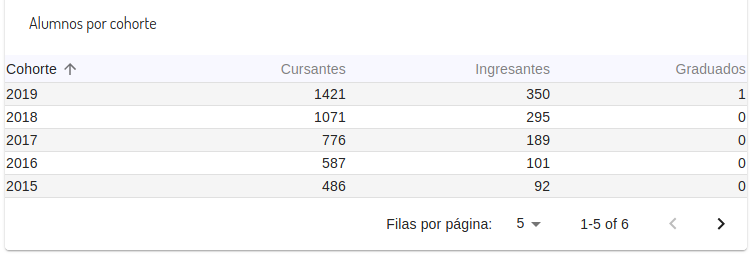
\includegraphics[scale=0.4]{images/seguimiento-academico/sa-alumnos-cohorte.png}
  \captionof{figure}{Tabla de estudiantes por cohorte}
  \label{fig:sa-alumnos-cohorte}
\end{figure}

\paragraph{Ingresantes por cohorte} \mbox{}\\
La siguiente es una tabla que detalla año a año de la carrera, qué cantidad de ingresantes hubo  (Figura~\ref{fig:sa-ingresantes-cohorte}).

\begin{figure}[H]
  \centering
    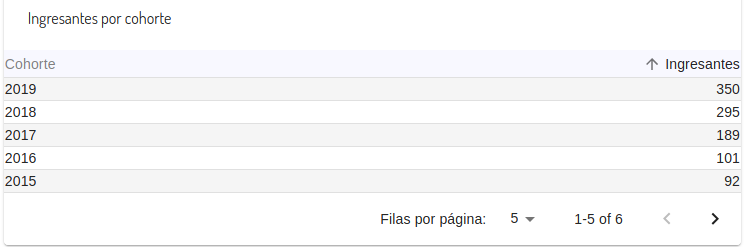
\includegraphics[scale=0.4]{images/seguimiento-academico/sa-ingresantes-cohorte.png}
  \captionof{figure}{Tabla de ingresantes por cohorte}
  \label{fig:sa-ingresantes-cohorte}
\end{figure}

\paragraph{Materias que demoran la formación} \mbox{}\\
La siguiente tabla muestra un puntaje por materia en base a su porcentaje de aprobación y sobre la dependencia que tienen otras materias sobre ésta para ser cursadas  (Figura~\ref{fig:sa-materias-traba}).

\begin{figure}[H]
  \centering
    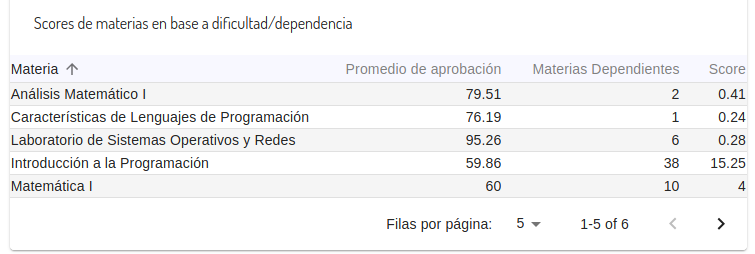
\includegraphics[scale=0.4]{images/seguimiento-academico/sa-materias-traba.png}
  \captionof{figure}{Tabla de ingresantes por cohorte}
  \label{fig:sa-materias-traba}
\end{figure}


\subsubsection{Visualización por materia}

Se dispone de un formulario para realizar un reporte, donde el usuario puede seleccionar entre sus carreras disponibles, luego ingresa el código de materia a analizar y una fecha de inicio y fin. De esta forma se analizará solo en el rango de fechas que se eligió.

Una vez que el formulario fue completado, se muestran los siguientes gráficos.

\paragraph{Estadísticas básicas de materia} \mbox{}\\
El siguiente gráfico muestra en forma de columnas los resultados de los estudiantes en el rango seleccionado. Se puede observar la cantidad de aprobados, ausentes, desaprobados y cuántos faltan cursarla  (Figura~\ref{fig:sa-datos-basico}).

\begin{figure}[H]
  \centering
    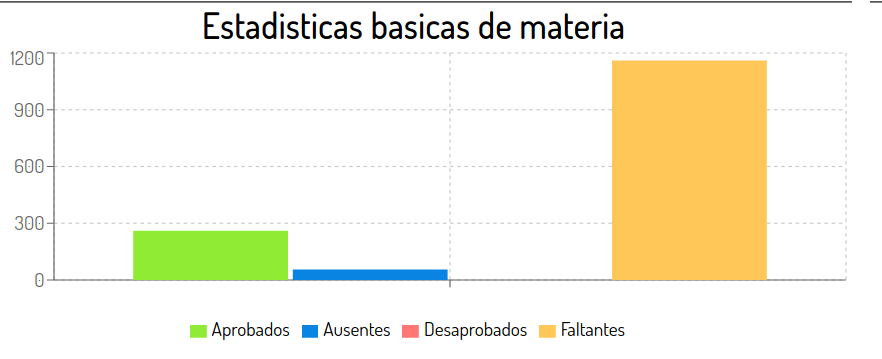
\includegraphics[scale=0.4]{images/seguimiento-academico/sa-datosbasicos.png}
  \captionof{figure}{Estadísticas básicas de la materia}
  \label{fig:sa-datos-basico}
\end{figure}

\paragraph{Detalle de aprobación} \mbox{}\\
El siguiente gráfico muestra en forma de columnas de qué forma aprobaron los estudiantes esa materia en el rango seleccionado. Se puede observar cuántos promocionaron en otra carrera, cuántos promocionaron, cuántos aprobaron un exámen equivalente, cuántos con una equivalencia equivalente y cuántos con exámen  (Figura~\ref{fig:sa-detalle-aprobacion}).

\begin{figure}[H]
  \centering
    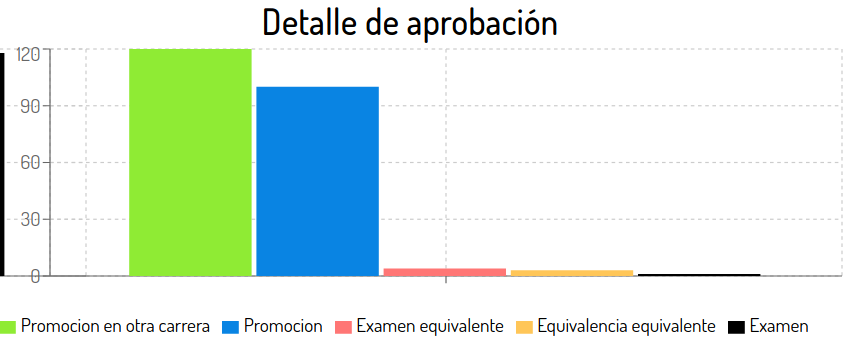
\includegraphics[scale=0.4]{images/seguimiento-academico/sa-detalleaprobacion.png}
  \captionof{figure}{Detalle de aprobación de la materia}
  \label{fig:sa-detalle-aprobacion}
\end{figure}

\paragraph{Dispersión de notas con respecto al promedio} \mbox{}\\
Este gráfico muestra en forma de dispersión la evolución de los estudiantes con respecto a su promedio.

\subsubsection{Visualización por estudiante}
Se dispone de un formulario para realizar un reporte, donde el usuario puede seleccionar entre sus carreras disponibles, luego ingresa el legajo del estudiante a analizar, un plan de estudios, y una fecha de inicio y fin. De esta forma, se analizará sólo en el rango de fechas que se eligió.

Una vez que el formulario fue completado, se muestran los siguientes gráficos.

\paragraph{Desempeño del estudiante} \mbox{}\\
El siguiente gráfico muestra el desempeño del estudiante semestralmente dentro del rango seleccionado  (Figura~\ref{fig:sa-detalle-aprobacion}).
\begin{figure}[H]
  \centering
    \includegraphics[scale=0.4]{images/seguimiento-academico/sa-desempeño.png}
  \captionof{figure}{Detalle de aprobación}
  \label{fig:sa-detalle-aprobacion}
\end{figure}

\paragraph{Porcentaje de carrera} \mbox{}\\
Se muestra el porcentaje de aprobación de la carrera en forma de tarjeta informativa.

\paragraph{Porcentajes de aprobación por área} \mbox{}\\
El siguiente gráfico de radar muestra los porcentajes de aprobación del estudiante dentro de las áreas de la carrera (Figura~\ref{fig:sa-porcentaje-area}).

\begin{figure}[H]
  \centering
    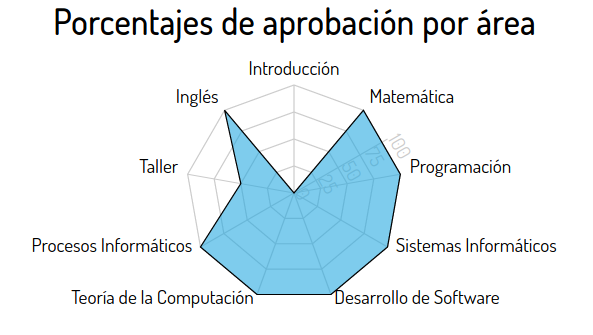
\includegraphics[scale=0.4]{images/seguimiento-academico/sa-porcentajesarea.png}
  \captionof{figure}{Porcentajes de aprobación por área}
  \label{fig:sa-porcentaje-area}
\end{figure}

\paragraph{Porcentajes de aprobacion por núcleo} \mbox{}\\
El siguiente gráfico de radar muestra los porcentajes de aprobación del estudiante dentro de los núcleos de la carrera (Figura~\ref{fig:sa-porcentaje-nucleo}).

\begin{figure}[H]
  \centering
    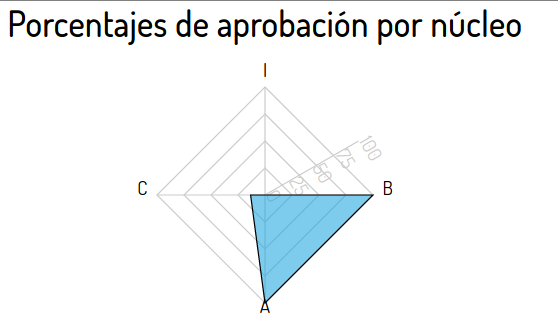
\includegraphics[scale=0.4]{images/seguimiento-academico/sa-porcentajesnucleo.png}
  \captionof{figure}{Porcentajes de aprobación por núcleo}
  \label{fig:sa-porcentaje-nucleo}
\end{figure}

\paragraph{Notas} \mbox{}\\
La siguiente tabla muestra las notas del estudiante dentro del rango seleccionado (Figura~\ref{fig:sa-notas}).

\begin{figure}[H]
  \centering
    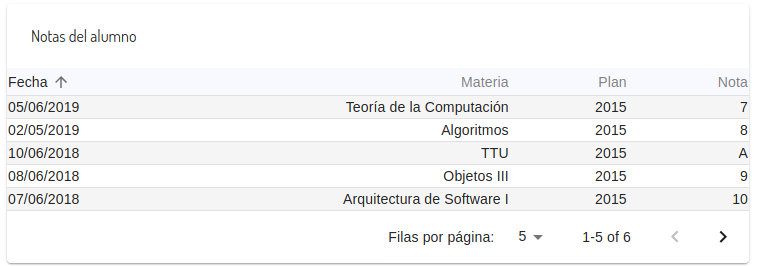
\includegraphics[scale=0.4]{images/seguimiento-academico/sa-notas.png}
  \captionof{figure}{Notas del estudiante}
  \label{fig:sa-notas}
\end{figure}



\section{Licencia}
El código será licenciado bajo una licencia libre avalada por la OSI (Open Source Initiative) y la
FSF (Free Software Foundation). El código fuente será subido de forma pública a un repositorio
de código online de la UNQ para el libre acceso de todo aquel que desee utilizar, estudiar,
modificar, copia, redistribuir, mezclar, publicar o sublicenciar el software en cuestión.

\section[Conclusiones]{Conclusiones}
		\chapter{Pruebas realizadas}
\label{sec:implementacion}

\section[Pruebas y resultados]{Pruebas y resultados}

\subsection[Resultados esperados]{Resultados esperados}

Se espera con este desarrollo tener un sistema capaz de brindarle datos a todos los interesados. Para que esto se cumpla, la implementación tiene que ser capaz de manejar todos los pedidos que recibe y responder en consecuencia. 
Si bien la problemática inicial implica que sólo se consultarán datos para analizarlos y ser visualizados por los directores de las carreras de la Universidad Nacional de Quilmes, no hay que descartar que pueda ser extendido dado su potencial.
Para garantizar que todo funcione de manera correcta se realizaron diferentes pruebas con escenarios cambiantes.
Para todas las pruebas se usaron los mismos URIs y se realizaron sobre una base de datos con 1.424 alumnos y 13.234 materias cursadas por estos alumnos.
La arquitectura utilizada para las pruebas se asemeja a la que dispondrá a la hora de la implementación.


\break
\subsection{Pruebas con 100 usuarios simultáneos}
\break
En primer lugar, se realizó una prueba en la cual 100 usuarios simultáneos se encuentran haciendo pedidos al núcleo, el cual está desplegado en una sola instancia de docker.
Esta prueba duró 5 minutos y los resultados se muestran a continuación.


\subsubsection{Resultados generales de la prueba}
\begin{table}[!htbp]
    \centering
    \makegapedcells
    \begin{tabular}{|c|c|c|c|}
    \hline
    Nombre del Pedido & Cantidad & Errores (\%) & Tiempo Promedio (ms) \\ \hline
    Total & 6825 & 3.06\% & 23469.53 \\ \hline
    Carrera | Nº cursantes & 381 & 6.56\% & 27740.51\\ \hline
    Carrera | Nº graduados & 345 & 3.77\% & 25571.40\\ \hline
    Carrera | Nº ingresantes & 477 & 1.89\% & 23485.62\\ \hline
    Carrera | Nº postulantes & 408 & 3.43\% & 22162.30\\ \hline
    Plan | Materias necesarias & 292 & 2.05\% & 21886.82\\ \hline
    Planes de carrera & 232 & 0.43\% & 18554.02\\ \hline

    \end{tabular}
    \caption{Pruebas realizadas con 100 usuarios simultáneos durante 5 minutos}
    \label{tab:tabla_planes}
\end{table}

En este caso el núcleo fue capaz de resolver todos los pedidos y responder sin problemas.

\subsubsection{Resultados sobre el uso de recursos durate la prueba}
\begin{table}[!htbp]
    \centering
    \makegapedcells
    \begin{tabular}{|c|c|c}
    \hline
    Contenedor & CPU & Memoria (MB)\\ \hline
    Núcleo & 68\% & 55 \\ \hline
    \end{tabular}
    \caption{Recursos en promedio consumidos por el contenedor durante la prueba}
    \label{tab:tabla_planes}
\end{table}

En promedio utilizó un 68\% del CPU y 55MB de memoria RAM.


\subsubsection{APDEX de la prueba}

APDEX (Índice de Performance de la Aplicación, por sus siglas en inglés) es un estandard abierto para medir la performance de una a aplicación de software. Su propósito es convertir las mediciones en información sobre la satisfacción del usuario, al especificar una forma uniforme de analizar e informar sobre el grado en que el rendimiento medido cumple con las expectativas del usuario.
Para realizar una medición APDEX, es necesario establecer un tiempo \emph{satisfactorio} y un tiempo \emph{tolerable}.
Una vez establecidos estos valores y tendo los resultados de la prueba, se calcula el índice:

\begin{align*}
  Apdex = \frac{Satisfactorios + \frac{Tolerables}{2}}{Total}\\
\end{align*}
\break
\begin{table}[!htbp]
    \centering
    \makegapedcells
    \begin{tabular}{|c|c|c}
    \hline
    APDEX Total & Tolerancia & Frustración\\ \hline
    0.064 & 2 seg & 3 seg \\ \hline
    \end{tabular}
    \caption{APDEX de la prueba con 100 usuarios durante 5 minutos}
    \label{tab:tabla_planes}
\end{table}


\break

\subsection{Pruebas con 500 usuarios simultáneos}
Luego de la primer prueba, se realizó una segunda en la cual 500 usuarios simultáneos se encuentran haciendo pedidos al núcleo, el cual está desplegado en una sola instancia de docker.
Esta prueba duró 10 minutos y los resultados se muestran a continuación.

\subsubsection{Resultados generales de la prueba}
\begin{table}[!htbp]
    \centering
    \makegapedcells
    \begin{tabular}{|c|c|c|c|}
    \hline
    Nombre del Pedido & Cantidad & Errores (\%) & Tiempo Promedio (ms) \\ \hline
    Total & 6825 & 3.06\% & 23469.53 \\ \hline
    Carrera | Nº cursantes & 381 & 6.56\% & 27740.51\\ \hline
    Carrera | Nº graduados & 345 & 3.77\% & 25571.40\\ \hline
    Carrera | Nº ingresantes & 477 & 1.89\% & 23485.62\\ \hline
    Carrera | Nº postulantes & 408 & 3.43\% & 22162.30\\ \hline
    Plan | Materias necesarias & 292 & 2.05\% & 21886.82\\ \hline
    Planes de carrera & 232 & 0.43\% & 18554.02\\ \hline

    \end{tabular}
    \caption{Pruebas realizadas con 500 usuarios simultáneos durante 10 minutos}
    \label{tab:tabla_planes}
\end{table}


\subsubsection{Resultados sobre el uso de recursos durate la prueba}
\begin{table}[!htbp]
    \centering
    \makegapedcells
    \begin{tabular}{|c|c|c}
    \hline
    Contenedor & CPU & Memoria (MB)\\ \hline
    Núcleo & 77\% & 55 \\ \hline
    \end{tabular}
    \caption{Recursos en promedio consumidos por el contenedor durante la prueba}
    \label{tab:tabla_planes}
\end{table}

\subsubsection{APDEX de la prueba}
\begin{table}[!htbp]
    \centering
    \makegapedcells
    \begin{tabular}{|c|c|c}
    \hline
    APDEX Total & Tolerancia & Frustración\\ \hline
    0.012 & 500ms & 1sec 500ms \\ \hline
    \end{tabular}
    \caption{APDEX de la prueba con 500 usuarios durante 10 minutos y una instancia de la aplicación}
    \label{tab:tabla_planes}
\end{table}

\subsection{Pruebas con 500 usuarios simultáneos}
Luego de la primer prueba, se realizó una segunda en la cual 500 usuarios simultáneos se encuentran haciendo pedidos al núcleo, el cual está desplegado en una sola instancia de docker.
Esta prueba duró 10 minutos y los resultados se muestran a continuación.

\subsubsection{Resultados generales de la prueba}
\begin{table}[!htbp]
    \centering
    \makegapedcells
    \begin{tabular}{|c|c|c|c|}
    \hline
    Nombre del Pedido & Cantidad & Errores (\%) & Tiempo Promedio (ms) \\ \hline
    Total & 6825 & 3.06\% & 23469.53 \\ \hline
    Carrera | Nº cursantes & 381 & 6.56\% & 27740.51\\ \hline
    Carrera | Nº graduados & 345 & 3.77\% & 25571.40\\ \hline
    Carrera | Nº ingresantes & 477 & 1.89\% & 23485.62\\ \hline
    Carrera | Nº postulantes & 408 & 3.43\% & 22162.30\\ \hline
    Plan | Materias necesarias & 292 & 2.05\% & 21886.82\\ \hline
    Planes de carrera & 232 & 0.43\% & 18554.02\\ \hline

    \end{tabular}
    \caption{Pruebas realizadas con 500 usuarios simultáneos durante 10 minutos}
    \label{tab:tabla_planes}
\end{table}
\subsubsection{Resultados sobre el uso de recursos durate la prueba}
\begin{table}[!htbp]
    \centering
    \makegapedcells
    \begin{tabular}{|c|c|c}
    \hline
    Contenedor & CPU & Memoria (MB)\\ \hline
    Núcleo-1 & 67\% & 54 \\ \hline
    Núcleo-2 & 68\% & 54 \\ \hline
    \end{tabular}
    \caption{Recursos en promedio consumidos por los contenedores durante la prueba}
    \label{tab:tabla_planes}
\end{table}
\subsubsection{APDEX de la prueba}
\begin{table}[!htbp]
    \centering
    \makegapedcells
    \begin{tabular}{|c|c|c}
    \hline
    APDEX Total & Tolerancia & Frustración\\ \hline
    0.067 & 500ms & 1sec 500ms \\ \hline
    \end{tabular}
    \caption{APDEX de la prueba con 500 usuarios durante 10 minutos y dos instancias de la aplicación}
    \label{tab:tabla_planes}
\end{table}
\break
\section{Conclusión sobre las pruebas}

Esto es una conclusion


		\chapter{Conclusiones}
\label{sec:conclusiones}

\section[Conclusiones]{Conclusiones}

A lo largo de esta tesis se han investigado numerosas herramientas de software para construir una solución para la centralización, disposición, análisis y visualización de datos académicos.

En primer lugar, se pensó una solución como servicios independientes, intercambiables y escalables según la necesidad. Esto facilita que si en un futuro aparece una tecnología superadora para una tarea en particular, sólo se tenga que reemplazar ese servicio.

Se ha logrado crear un Núcleo que almacena datos y los entrega a través de una API REST, la cual puede ser consmumida por usuarios que tengan los permisos correspondientes.

Se creó un servicio para el análisis de los datos consultados al núcleo, el cual también entrega el resultado del procesamiento de esos datos para que puedan ser consumidos.

Luego, se creó un servicio que facilita la visualización de los datos procesados. Éste consume los datos del módulo de análisis y muestra los resultados en forma de gráfico de columnas, gráfico de tortas, gráficos de radar, gráficos de puntos, tablas, etc.

Este conjunto de servicios les permite a las partes interesadas consultar la información, modificarla, consultar métricas sobre carreras, materias y estudiantes de forma individual o colectiva y consultar datos sobre períodos en particular.
Esta solución se ajusta perfectamente a la arquitectura provista por la Universidad.

Se ha aprendido acerca de la importancia de la disposición de los datos y cómo esto puede ayudar a tomar decisiones tempranas sobre la vida académica de la Universidad Nacional de Quilmes, sus carreras, sus materias y su alumnado.


\section[Lineas de Trabajos futuros]{Lineas de Trabajos futuros}

Dado que el sistema se pensó de forma tal que se pueda extender fácilmente, y que sus datos puedan ser consultados por otros servicios, existen varias mejoras y puntos de extensión que se detallan a continuación:

\subsection[Aplicación para estudiantes]{Aplicación para estudiantes}

Podría existir una aplicación para que usen los estudiantes (puede ser móvil o web), donde puedan consultar su historial dentro de la Universidad. Si bien esta tarea se puede realizar en Guaraní, se podría integrar con servicios que brinda la universidad, como la consulta del saldo disponible en la tarjeta de la UNQ, notificaciones con novedades y noticias que estén relacionadas únicamente con los estudiantes.
Esta aplicación, a su vez, puede tener un aspecto mas social: que los estudiantes pongan tips y consejos sobre las materias.
Además, podría recibir feedback sobre los que ya cursaron, los horarios, las comodidades, la calidad de enseñanza, etc.

\subsection[Integración con Guaraní]{Integración con Guaraní}

Sería muy conveniente poder conectar el Núcleo con Guaraní a través de una API web. En la actualidad no existe dicha API, pero con el lanzamiento de Guaraní 3 debería ser posible. De esta forma, no se deberían importar más los datos a través de planillas, sino que se haría de forma automática a través del Núcleo.

\subsection[Integración con sistema de encuestas de inscripción]{Integración con sistema de encuestas de inscripción}

El sistema actual que utilizan algunas carreras de la UNQ para consultar las posibles inscripciones de los estudiantes debería ser integrado al núcleo para que consuma datos, y luego debería enviar los resultado para luego con esa información mostrar métricas a los directores de carreras. 


\subsection[GraphQL en el núcleo]{GraphQL en el núcleo}

GraphQL es un lenguaje de queries para APIs, donde los clientes definen precisamente qué datos quieren en lugar de recibir todos los datos disponibles. Esto significaría una reducción en el tamaño de respuesta de la API del núcleo.

\subsection[Proveedor de identidad (IDP)]{Proveedor de identidad (IDP)}

Dado que el potencial de extensión es amplio, una buena forma de desligarle responsabilidades al núcleo es crear un proveedor de identidad. En lugar de los usuarios identificarse ante el núcleo y que este les provea un token, debería hacerlo un servicio independiente que tenga conocimiento de todos los usuarios, y éste se encargue de validar quién puede ingresar y quién no, y qué permisos tiene.

\subsection[Acceso Centralizado]{Acceso Centralizado}

Una vez que exista el IDP, sería muy útil un acceso centralizado. Esto significa que, una vez que el usuario se identifica con el IDP, éste lo considera *logueado* en todas las aplicaciones que el usuario tiene acceso. Cuando ingrese a otra aplicación, automáticamente el IDP lo deja ingresar.




	\backmatter
		\bibliographystyle{IEEEtran}
		%\bibliographystyle{plain}     %You may prefer \bibliographystyle{alpha}
		%\bibliographystyle{alpha}
		%\bibliographystyle{babalpha}
		\bibliography{books}
		\nocite{*}
		\chapter{Anexos}

\section{Pantallas básicas del Núcleo}


\subsubsection{Login}
\begin{figure}[h!]
  \centering
    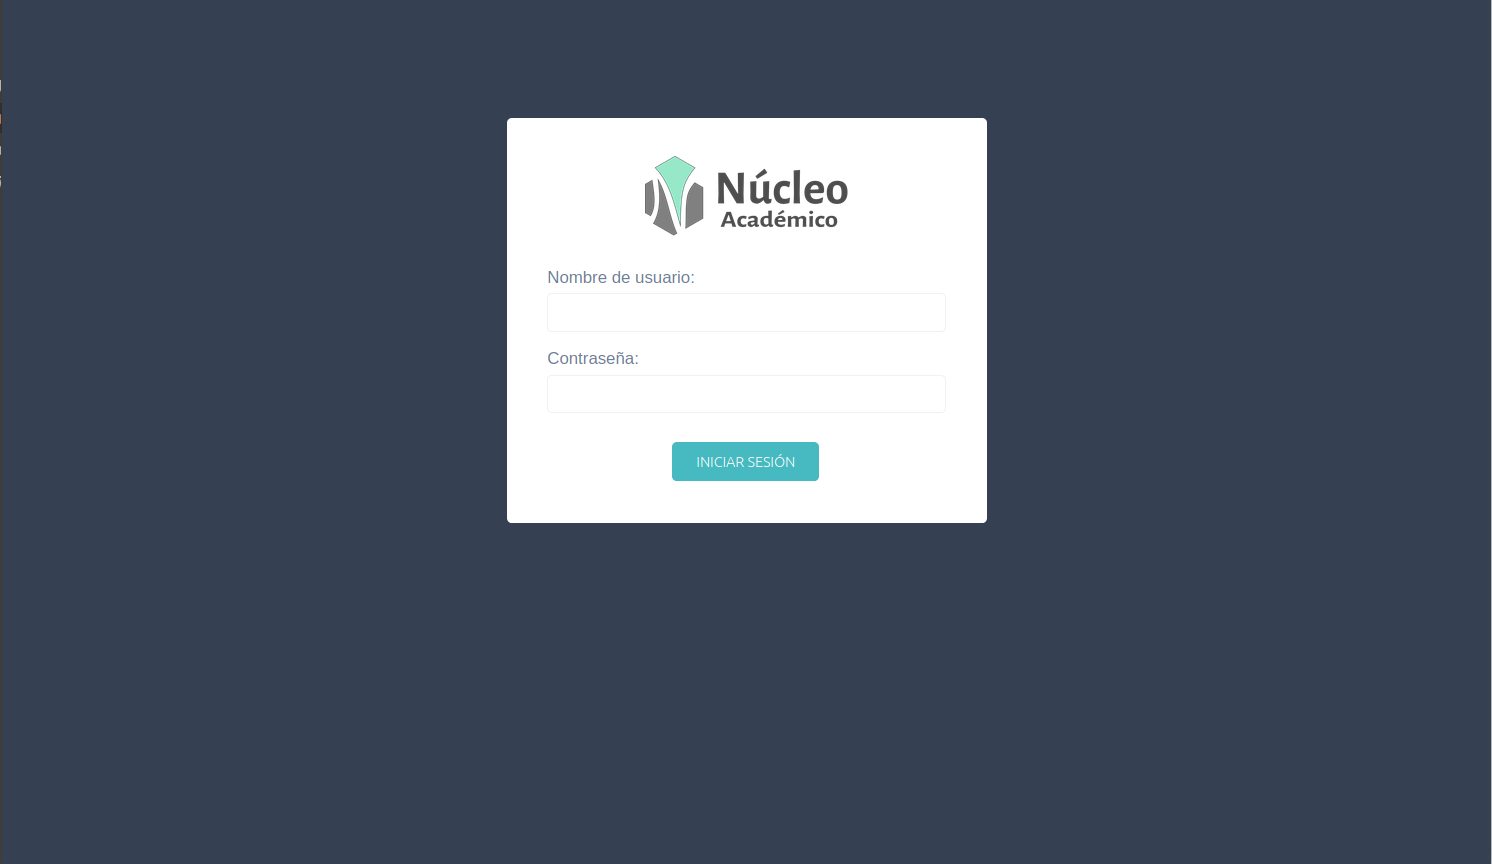
\includegraphics[scale=0.3]{images/nucleo/nucleo-login.png}
  \captionof{figure}{Pantalla de login}
  \label{fig:nucleo-login}
\end{figure}

\subsubsection{Home}
\begin{figure}[h!]
  \centering
    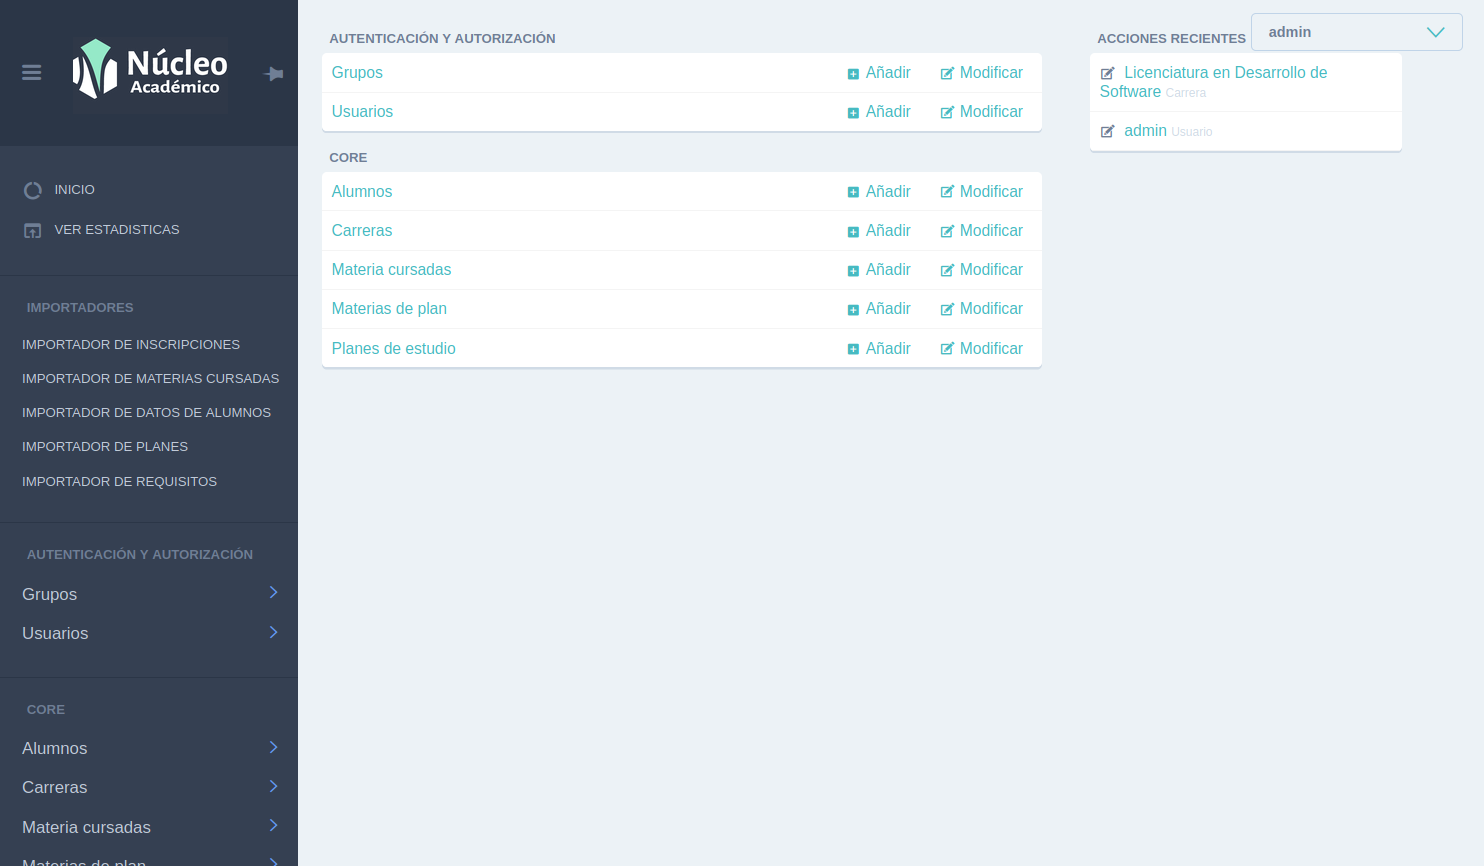
\includegraphics[scale=0.3]{images/nucleo/nucleo-home.png}
  \captionof{figure}{Pantalla principal del admin}
  \label{fig:nucleo-home}
\end{figure}

\subsubsection{Importadores}
\begin{figure}[h!]
  \centering
    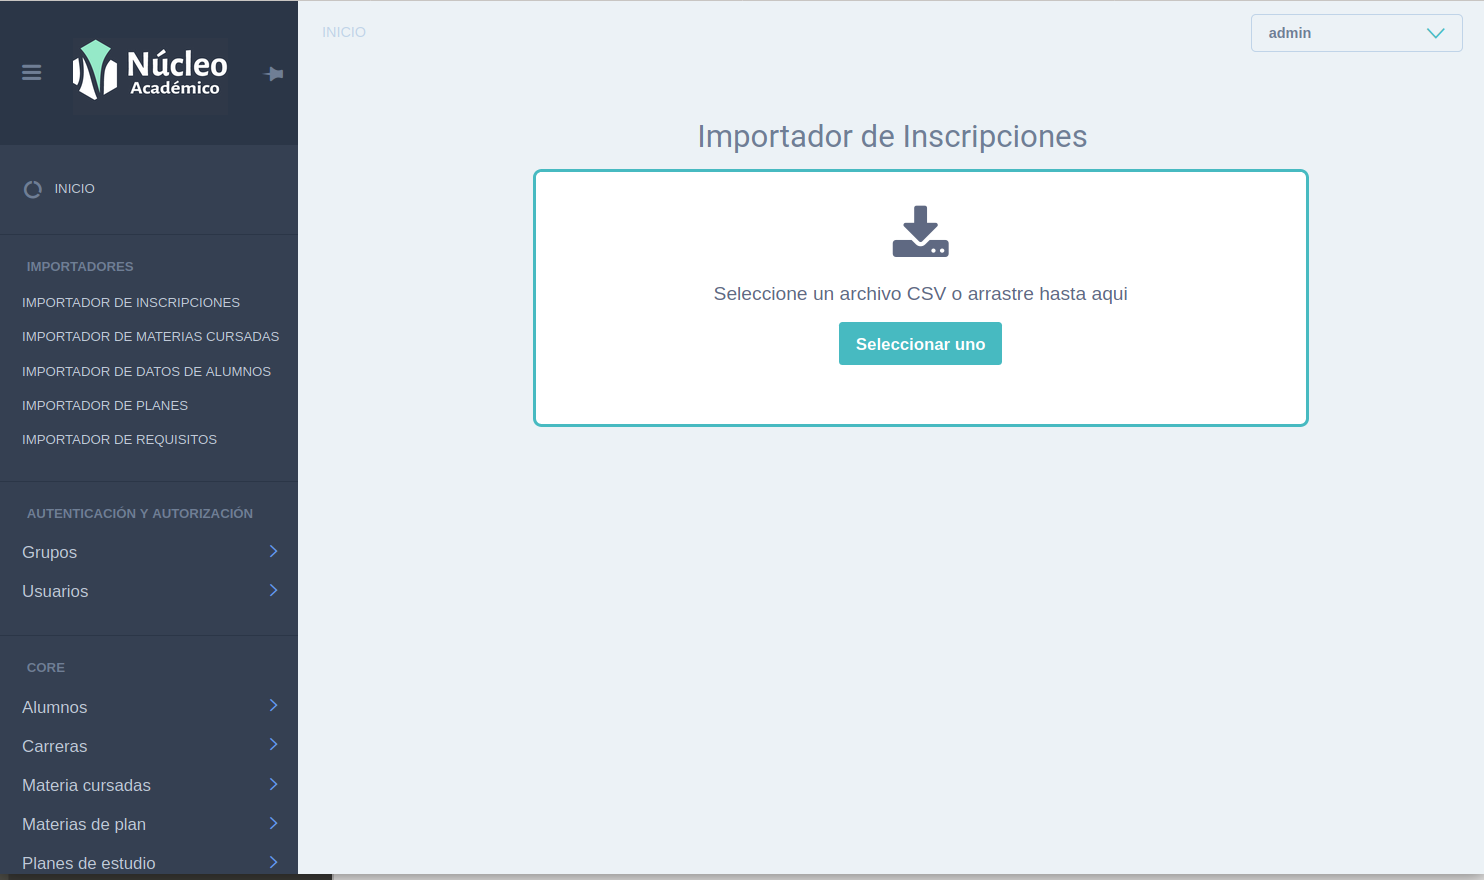
\includegraphics[scale=0.3]{images/nucleo/nucleo-importador.png}
  \captionof{figure}{Pantalla de importadores}
  \label{fig:nucleo-importador}
\end{figure}

\subsubsection{Listado}
\begin{figure}[h!]
  \centering
    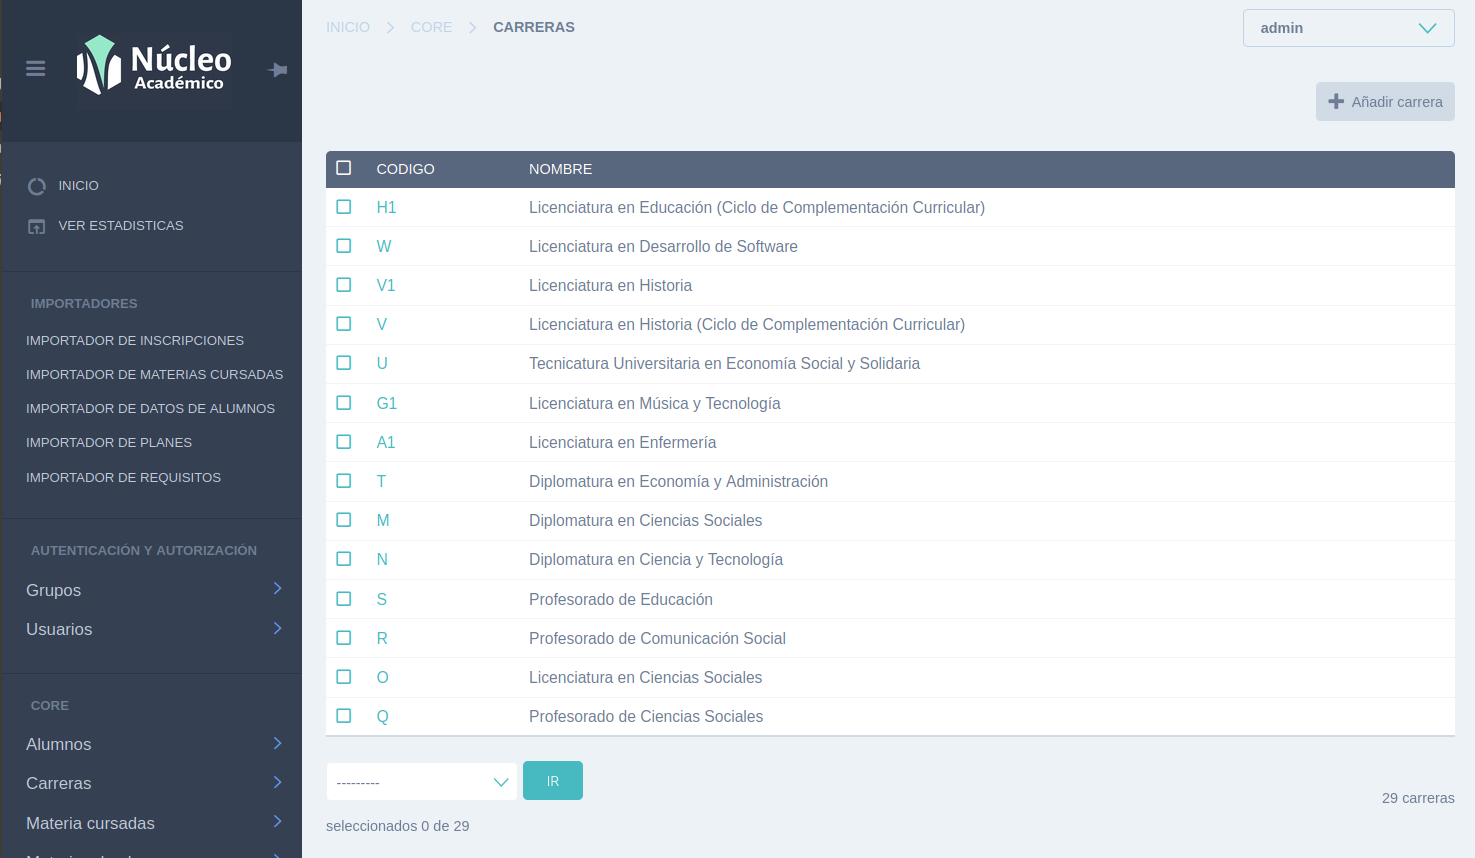
\includegraphics[scale=0.3]{images/nucleo/nucleo-list.png}
  \captionof{figure}{Pantalla de listados}
  \label{fig:nucleo-listado}
\end{figure}

\subsubsection{Edicion}
\begin{figure}[h!]
  \centering
    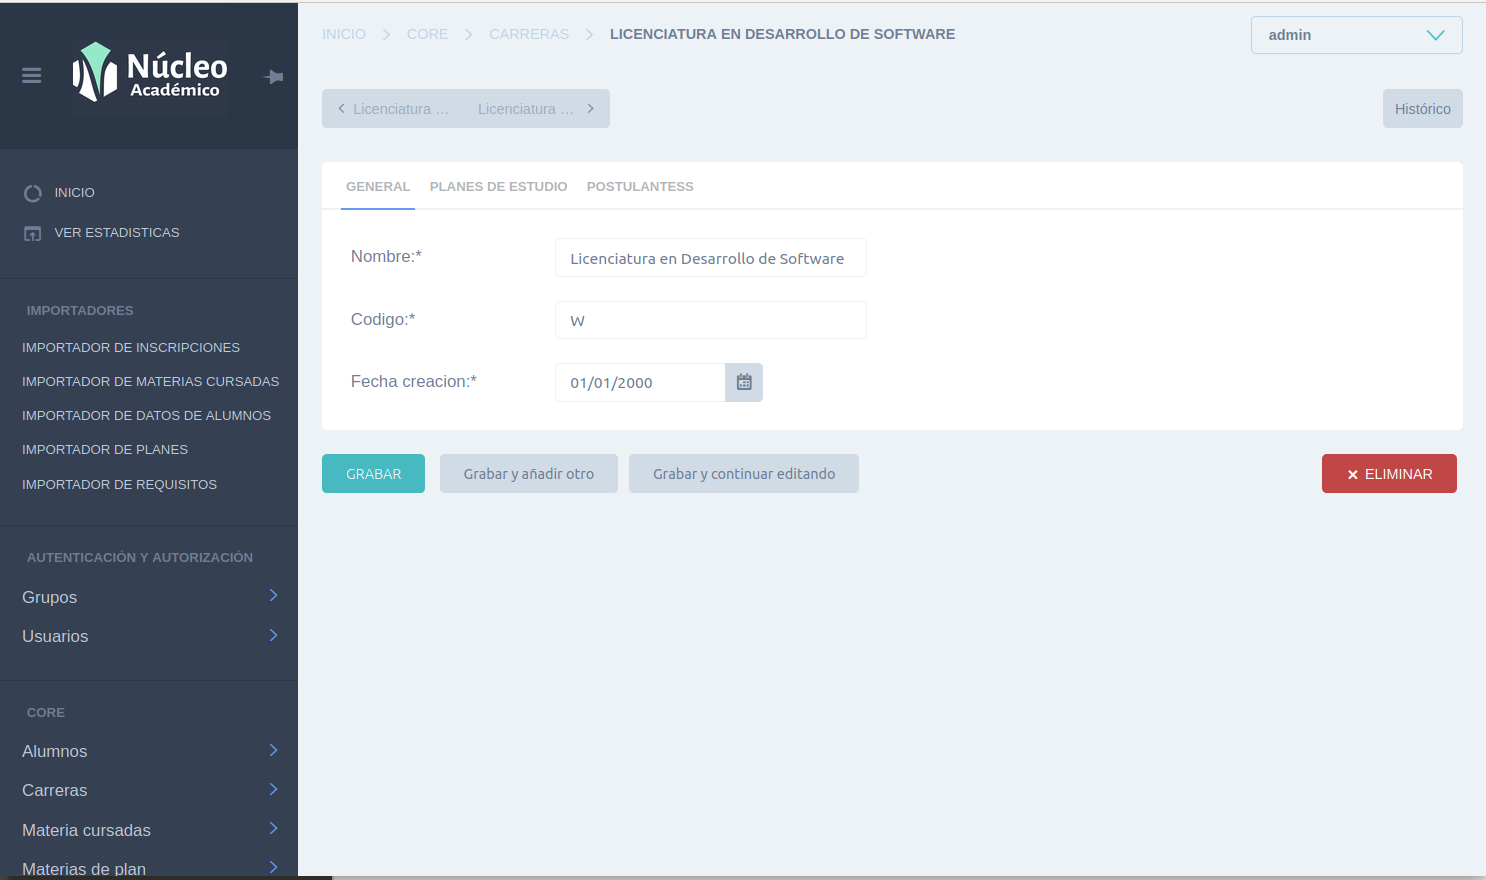
\includegraphics[scale=0.3]{images/nucleo/nucleo-edit.png}
  \captionof{figure}{Pantalla de edición}
  \label{fig:nucleo-edicion}
\end{figure}

\subsubsection{Pedir Token}
\begin{table}[!htbp]
    \centering
    \makegapedcells
    \begin{tabular}{|c|c|c|c|c|}
    \hline
    URI & Método & Parámetros & Content-Type \\ \hline
    api/token/ & POST & username,password & application/x-www-form-urlencoded \\ \hline
    \end{tabular}
    \caption{Método para pedir un token al núcleo}
    \label{tab:tabla_token}
\end{table}

\subsubsection{API}
\begin{table}[!htbp]
    \centering
    \makegapedcells
    \begin{tabular}{|c|c|c|}
    \hline
    URI & Método & Autorización\\ \hline
    carreras/<str:cc>/alumnos/ & GET & Bearer  \\ \hline
    carreras/<str:cc>/alumnos-completos/ & GET & Bearer  \\ \hline
    carreras/<str:cc>/planes/<int:plan\_anio>/ & GET & Bearer  \\ \hline
    carreras/<str:cc>/planes/<int:pa>/cantidad-materias-necesarias/ & GET & Bearer  \\ \hline
    carreras/<str:cc>/planes/ & GET & Bearer  \\ \hline
    carreras/<str:cc>/materiascursadas/ & GET & Bearer  \\ \hline
    carreras/<str:cc>/inscripciones/ & GET & Bearer  \\ \hline
    carreras/<str:cc>/cantidad-graduados/ & GET & Bearer  \\ \hline
    carreras/<str:cc>/cantidad-graduados/<int:anio>/ & GET & Bearer  \\ \hline
    carreras/<str:cc>/cantidad-cursantes/ & GET & Bearer  \\ \hline
    carreras/<str:cc>/cantidad-cursantes/<int:anio>/ & GET & Bearer  \\ \hline
    carreras/<str:cc>/cantidad-ingresantes/ & GET & Bearer  \\ \hline
    carreras/<str:cc>/cantidad-ingresantes/<int:anio>/ & GET & Bearer  \\ \hline
    carreras/<str:cc>/cantidad-postulantes/<int:anio>/ & GET & Bearer  \\ \hline
    carreras/<str:cc>/cantidad-postulantes/ & GET & Bearer  \\ \hline
    alumno/<str:legajo>/cursadas/ & GET & Bearer  \\ \hline
    alumno/<str:legajo>/inscripciones/ & GET & Bearer  \\ \hline
    materia/<str:codigo>/alumnos/ & GET & Bearer  \\ \hline
    \end{tabular}
    \caption{Métodos para pedir datos. (cc: código de carrera, pa: plan año)}
    \label{tab:tabla_api}
\end{table}

	%opcional
\end{document}